\chapter{Standard Model Backgrounds}
\label{chap:backgrounds}

\section{Signal Region Background Composition}
\label{sec:Bkg:Compositiion}

The dominant background in all signal region bins is SM $\ttbar$, accounting for $70$ percent of all backgrounds in the signal region.  The next most prevalent background is W+jets which accounts for 9\% of all signal region backgrounds but can reach up to 24\% percent in high $\RISR$ bins. The breakdown of background composition is given in Table \ref{tab:SRBkg} \\

\begin{table}[htpb]
  \begin{center}
    \def\arraystretch{1.4}%
    \begin{tabular}{c||c|c|c|c|c|c|} \hline\hline
      \RISR Range  & 0.3-0.4 & 0.4-0.5 & 0.5-0.6 & 0.6-0.7 & 0.7-0.8 \\  \hline
      t\tbar         &  61\% & 78\% & 74\% & 60\% & 64\%  \\  \hline
      $W$+jets  &  4\%   & 7\%   & 10\% & 24\% & 21\%  \\  \hline 
      $Z$+jets   &  2\%   & 3\%   & 4\%  & 6\%    & 9\%  \\  \hline
      Single top & 2\%    & 4\%   & 6\%  & 9\%    & 6\% \\ \hline
      $\ttV$        & 1\%   & 2\%    & 3\%  & 1\%    & 0\%  \\ \hline
      QCD         & 22\% &  5\%   & 2\%  & 0\%    & 0\%  \\ \hline
      dibosons  & 8\%    & 1\%    &  1\% & 0\%    & 0\%  \\ \hline \hline
    \end{tabular}
  \caption{Standard Model background composition in the signal region ~\ref{tab:SRBkg}.   }
  \end{center}
  \label{tab:SignalRegion}
\end{table}%


\section{Using Control and Validation Regions to Estimate Background in the Signal Region}
\label{sec:Bkg:Tech}

\indent We use both data and MC based background estimation technique for estimating background rates in the signal region.  A common partially data driven technique directly measures the amount of background in kinematically similar control regions in data.  Once we know the background rates in the control region in data, we can then extrapolate to the signal region using MC predictions. \\

\indent We determined the background rate through a simultaneous fit to all control regions and signal region when setting limits or calculating discovery significances.  The background rate will be mainly constrained by the control regions because the control regions have significantly higher statistics then the signal region.  \\

\indent We also perform a background only fit to estimate the background rates.  The background only fit extracts a normalization factor for each background by simultaneously fitting all control regions.  The normalization factors are then applied to the expected background rates in the signal region.  The background only fit results may differ from the combined fit. However the two estimate should be similar as long as the control regions are well designed.   A more detailed explanation of the control regions, signal region and fitting procedures are covered in the statistical analysis Chapter \ref{chap:statistics}.  \\

%\indent We can get a quick estimate of the amount of background in the SR by calculating the transfer factor and normalization factor defined in equation \ref{eqn:TF} and \ref{eqn:mu}. \\

%\begin{equation}
%T = \frac{N_{MC}^{SR}}{N_{MC}^{CR}}
%\label{eqn:TF}
%\end{equation}
%\begin{equation}
%\mu_{MC} = \frac{N_{data}^{CR}-N_{non-ttbar MC}^{CR}}{N_{ttbar~MC}^{CR}}
%\label{eqn:mu}
%\end{equation}

%\indent We normalize the MC in CR to data with a normalization scale factor $\mu$ defined in equation \ref{eqn:mu}.  We then apply the transfer factor to predict the amount of $\ttbar$ we expect to see in the SR.  This is mathematically equivalent to simply normalizing the amount of $\ttbar$ MC in the SR by the scale factor derived in the CR because the transfer factor is the just the relative rates of MC in the SR and CR.   \\

%\indent This simplified result may differ slightly from the combined fit.  However the two estimate should be similar as long as the CRs are well designed and consists mainly of a single type of background. \\

\indent We use control regions to estimate the dominant $\ttbar$ background and subdominant $W$+jet, single top, and ttV backgrounds.  Details on the $\ttbar$ background is found in section \ref{sec:Bkg:ttbar}.  \\

\indent $Z$+jets and dibosons contribute less then 5 percent of all backgrounds in the signal region.  Therefore these backgrounds are estimated using MC alone and apply an additional 50 percent theory uncertainty for these two samples.  Finally QCD multijet background is estimated using the {\tt Jet Smearing} method described in section \ref{sec:Bkg:QCD}.  Details on the treatment of each subdominant background can be found in section \ref{sec:Bkg:sub}.\\

%\indent The scale factors for each background derived from the simultaneous fit to the CR are given in table \ref{table.scale.factors}. $\ttbar$ background is scaled down by 0.707 because the MC over estimates the amount of $\ttbar$ that is produced with strong ISR. \\

%\begin{table}
%  \begin{center}
 %   \begin{tabular*}{\textwidth}{@{\extracolsep{\fill}}lr}
      \noalign{\smallskip}\hline\noalign{\smallskip}
      {\bf MC sample}           & Fitted scale factor        \\[-0.05cm] \hline
      ttbar &   $0.707 \pm 0.050$             \\
      W+jets &   $1.27 \pm 0.15$              \\
      Single top &   $1.17 \pm 0.39$              \\
      ttbar$\gamma$ &   $1.29 \pm 0.20$              \\ \hline
    \end{tabular*}

%  \end{center}
%  \caption{MC scale factors for SM backgrounds.  Scale factors are derived by simultaneously fitting to all background CR using \intlumi\ \ifb of data.}
%  \label{table.scale.factors}
%\end{table}

\section{Dominant Background: Standard Model $t\tbar$}
\label{sec:Bkg:ttbar}

\indent The dominant background in this analysis is SM $\ttbar$.  After signal selection $\ttbar$ still accounts for $60-80$ percent of the background depending on $\RISR$ range.  This section covers in detail the properties and treatment of SM $\ttbar$ in this analysis.  The section \ref{sec:Bkg:ttbar:Pop} demonstrates that there exists two kinematically distinct populations of SM $\ttbar$, each with unique characteristics and observables.  Section \ref{sec:Bkg:ttbar:CR} describes how we are able to directly measure the amount of $\ttbar$ in the signal region using a one lepton control region.  \\

%Section \ref{sec:Bkg:ttbar:Sel} explores the kinematics of $\ttbar$ events after SR selection.  

%\indent The $\met>250 \gev$ requirement selects $\ttbar$ with boosted leptonic tops because a top at rest cannot produce a neutrino with 250 $\gev of $\pt$.  After zero lepton preselection, two kinematically distinct populations of $\ttbar$ exist.  One $\ttbar$ population use strong ISR to boost both tops. The other population uses boosts the leptonic top against the hadronic top in a back-to-back fashion. Section \ref{sec:Bkg:ttbar:Pop} describes these two kinematically distinct populations of $\ttbar$ in greater detail.   \\

%\indent Section \ref{sec:Bkg:ttbar:Sel} describes the signal selections used to remove the majority of $\ttbar$ background while retaining most of the signal.  These selection targets the larger and kinematically different population of $\ttbar$ that does not have strong initial state radiation.  $\ttbar$ with strong ISR appears more signal like and 90 percent of all $\ttbar$ backgrounds after SR selection are $\ttbar$ events with at least $400$ GeV of true initial state radiation.  These same selections are also very effective at removing subdominant SM backgrounds such as W+jets and Z+jets. \\

%\indent Section \ref{sec:Bkg:ttbar:CR} describes how we are able to directly measure the amount of $\ttbar$ background that is produced with strong initial state radiation in data using an one lepton control region.  We avoid relying on theory predictions on the amount of ISR $\ttbar$ is expected to produce.  In this way, the control region allows us to minimize the amount of systematic uncertainties in the SR. \\

\subsection{Two Kinematically Distinct Populations of $t\tbar$}
\label{sec:Bkg:ttbar:Pop}

\indent After the zero lepton preselection, 80 percent of $\ttbar$ events decay via the single hadronic tau channel.  $15$ percent of $\ttbar$ events decay via the single lepton channel where the lepton is an electron or a muon.  The lepton is later lost because either it has too low $\pt$ to be reconstructed, is removed because they are to close to another jet or is misreconstructed as a jet. The rest of the five percent are due to dileptonic decays. Fully hadronic $\ttbar$ is negligible after signal region selections because fully hadronic $\ttbar$ produces little intrinsic $\met$. \\

\indent  The $\met>250 \gev$ requirement in preselection selects for $\ttbar$ with a boosted leptonic top.  A top at rest simply do not have enough energy to produce a neutrino with 250 $\gev$ of $\pt$. The leptonic top can gain boost mainly through one of two ways.  Either the leptonic top recoils in a back-to-back fashion against the hadronic top or both tops can recoil against strong ISR.  \\

%\indent Most $\ttbar$ events has one top that decays leptonically and the other top decaying fully hadronically after zero lepton preselection. The leptonic top also produces a neutrino that satisfies the $250$ GeV of \MET requirement.  In most cases, the lepton is a tau that decays hadronically and registers as jet in calorimeter instead of a lepton.  In a smaller fraction of events a muon or electron is produced but the lepton is lost because of a number of reasons.  For example, the lepton can have too low $\pt$ to be reconstructed, or can be removed because they were to close to another jet or an electron is misreconstructed as a jet.  \\

%\indent Regardless of the exact decay channel, a top decaying at rest cannot generate enough momenta for the neutrino to have $250$ GeV of pt.  The top decaying via a tau or lepton, called the leptonic top, must therefore be boosted to have a high probability of satisfying the $250$ GeV \MET cut.  The leptonic top can gain this boost through one of two ways.  Either the leptonic top recoils in a back-to-back fashion against the hadronic top or both tops recoil against strong ISR.  \\

\indent In both situations the thrust axis, the axis of maximum back-to-back $\pt$, contains important information.  In the case where the leptonic is recoiling against the hadronic top, the thrust axis lines up along the top/anti-top's axis of back-to-back boost.  In the case where both tops are boosted by strong ISR, the thrust axis approximates the $\ttbar$ vs ISR boost direction. An artistic representation of the role of the thrust axis in each $\ttbar$ population can be seen in Figure \ref{fig:ttbar:2pop}. \\

\begin{figure}[h!]
  \centering
	\includegraphics[width=0.65\textwidth]{./figures/strategy/ttbar_2pop.png}
	\caption[Schematic depiction of the top/anti-top back-to-back $\ttbar$ population and the $\ttbar$ plus strong ISR population after the zero lepton preselection.]{Schematic depiction of the top/anti-top back-to-back $\ttbar$ population and the $\ttbar$ plus strong ISR population after the zero lepton preselection. The two example events' thrust axes are aligned.  The hemisphere containing $\met$ has significantly higher jet multiplicities and total energy in $\ttbar$ plus strong ISR events. }
\label{fig:ttbar:2pop}
\end{figure}

\indent Only the leptonic top is boosted towards the same hemisphere as the $\met$ in $\ttbar$ with strong top/anti-top back-to-back boost.  In comparison, both tops are boosted towards the hemisphere containing $\met$ in the $\ttbar$ with strong ISR. Therefore $\ttbar$ plus strong ISR population has on average a much higher jet multiplicities and total energy in the hemisphere containing $\met$.  Hence, we can use observable such as $\NjV$ and $\MS$ to distinguish $\ttbar$ plus strong ISR events from top/anti-top back-to-back recoil events.   \\

%\subsection{Properties of SM $t\tbar$ in Signal Region}
%\label{sec:Bkg:ttbar:SR}

%\indent Stop signal is expected to have a higher jet multiplicities and energy in the hemisphere containing $\met$ then both $\ttbar$ populations.  The stringent SR requirements on the jet multiplicities and total energy of the sparticle hemisphere effectively eliminate the top/anti-top back-to-back $\ttbar$ population and also rejects approximately $2/3$ of $\ttbar$ plus strong ISR population.  A detailed explanation of SR design and performance can be found in chapter \ref{chap:SignalRegion}. \\

%\indent The $\ttbar$ events that survives the SR selections are composed of almost exclusively $\ttbar$ that are also produced with strong ISR.  Approximately 90 percent of the $\ttbar$ events in SR have an ISR $\pt$ of at least 400 $\gev$.  The distribution of true ISR $\pt$ for $\ttbar$ that survive the signal selections can be seen in figure \ref{fig:ttbar:SR:trueISRpt}.\\

%\begin{figure}[h!]
%  \centering
%	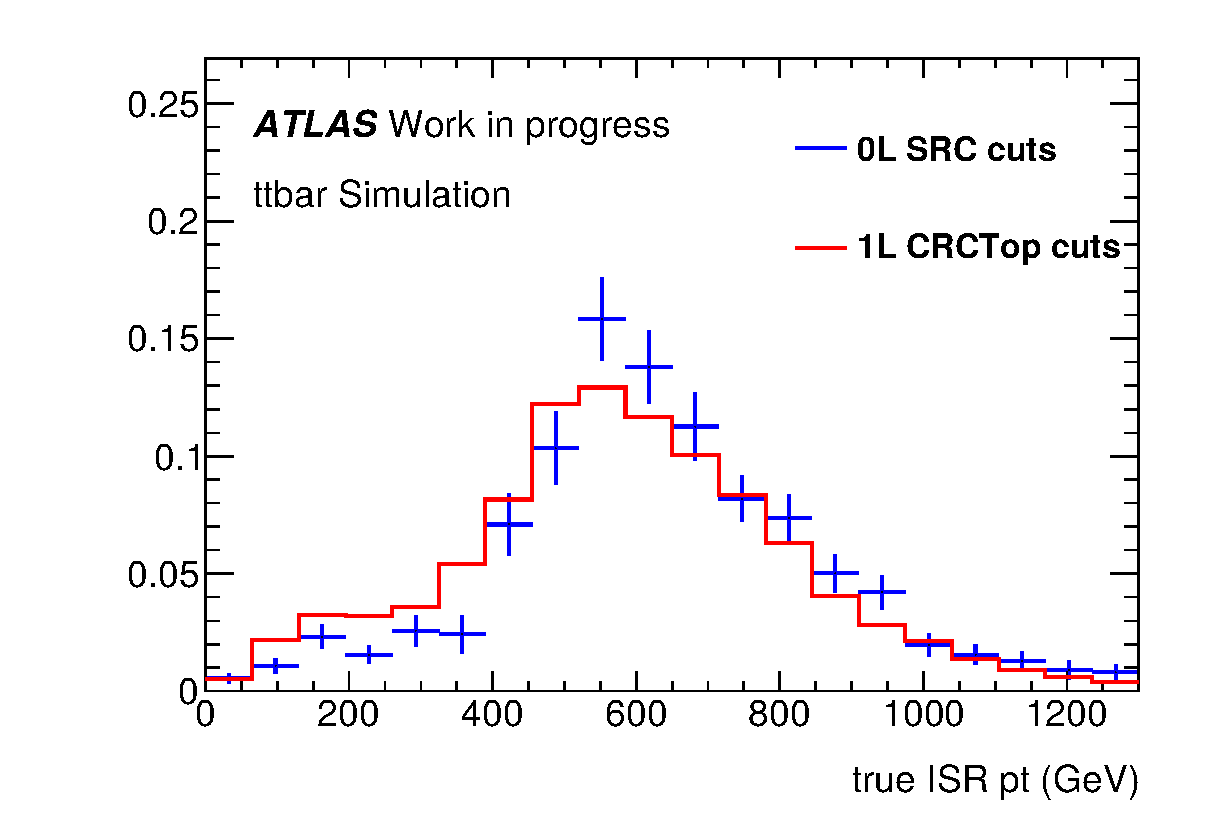
\includegraphics[width=0.65\textwidth]{./figures/ttbar/truePtISR_SRC_CRC_compare.eps}
%\caption{\label{fig:ttbar:CR:trueISRpt}{Distribution of true ISR $\pt$ for $\ttbar$ that survive the signal selections}}
%\end{figure}

%\indent In terms of branching fractions, the majority of $\ttbar$ branching fractions are to hadronic taus.  80 percent of the $\ttbar$ has one top decay via a single hadronic tau and the other top decays fully hadronically.  $15$ percent of the $\ttbar$ events decay via the single lepton channel where the lepton is an electron or a muon.  The lepton becomes lost because either it has too low $\pt$ to be reconstructed, removed because they were to close to another jet or is misreconstructed as a jet. The rest of the five percent composed of di-leptonic or lepton and tau $\ttbar$ events. Essentially no fully hadronic $\ttbar$ survives the zero lepton selection because fully hadronic $\ttbar$ do not make any hard neutrinos directly from the top decay.  \\
%\indent With such a large fraction of background coming from taus one might suspect setting up some sort of tau rejection.  However we found that a rejection based on loose tau IDs did not improve sensitivity.  The loss of signal was too large to justify the improvement in signal to background ratio.  The high jet multiplicity in signal gives a high probability of false positives.
%\indent Accepting mainly $\ttbar$ decay to hadronic taus gives a large boost signal to background due to branching fractions alone.  The two tops in signal events decay mainly through the fully hadronic channel.  Fully hadronic decays account for 44 percent of all $\ttbar$ decays.  On the other hand, the $\ttbar$ background mainly decay via hadronic taus which only accounts for about 10 of all $\ttbar$ decays.  We therefore gain a factor of 5 in signal to background ratio just by working in the zero lepton channel. This not only gains us a great boost in sensitivity in our SR.  It also allows us to design a $\ttbar$ control region with very similar selections to the SR but just in the single lepton channel.  We can avoid high signal contamination in our control region because both signal and background are mainly coming from single lepton decays in the one lepton channel.  As such, we no longer gain this factor of 5 in S/B based on branching fraction in the control region.  The details of the $\ttbar$ control region is described in section \ref{sec:Bkg:ttbar:CR} \\  

\subsection{Predicting the amount of $\ttbar$ in Signal Region using a One Lepton Control Region}
\label{sec:Bkg:ttbar:CR}

\indent Stop signal is expected to have a higher jet multiplicities and energy in the hemisphere containing $\met$ then both $\ttbar$ populations.  The stringent signal region requirements on the jet multiplicities and total energy of the sparticle hemisphere effectively eliminate the top/anti-top back-to-back $\ttbar$ population and also rejects approximately $2/3$ of $\ttbar$ plus strong ISR population.  A detailed explanation of SR design and performance can be found in chapter \ref{chap:SignalRegion}. \\

%The $\ttbar$ events that survives the signal selections are composed of almost exclusively $\ttbar$ that are also produced with strong ISR.  
\indent Approximately 90 percent of the $\ttbar$ events in the signal region have at least 400 $\gev$ of real ISR $\pt$.  A back of the envelope calculation shows that we need around 550-600 $\gev$ of ISR $\pt$ to boost the $\ttbar$ neutrino to above 250 $\gev$ of $\pt$.  The neutrino must share the total $\ttbar$ $\pt$ with the five other $\ttbar$ decay products and is not particularly efficient at absorbing ISR $\pt$.  \\

\indent Figure \ref{fig:ttbar:SR:trueISRpt_presel_SRC1} shows that the true ISR $\pt$ distribution for $\ttbar$ in the signal region peaks at approximately 550 $\gev$.  In comparison, the true ISR $\pt$ distribution after preselection peaks at zero and rapidly falls with increasing ISR $\pt$.  This demonstrates that the additional signal region requirements select mainly for $\ttbar$ with high ISR $\pt$.  \\

\begin{figure}[h!]
  \centering
	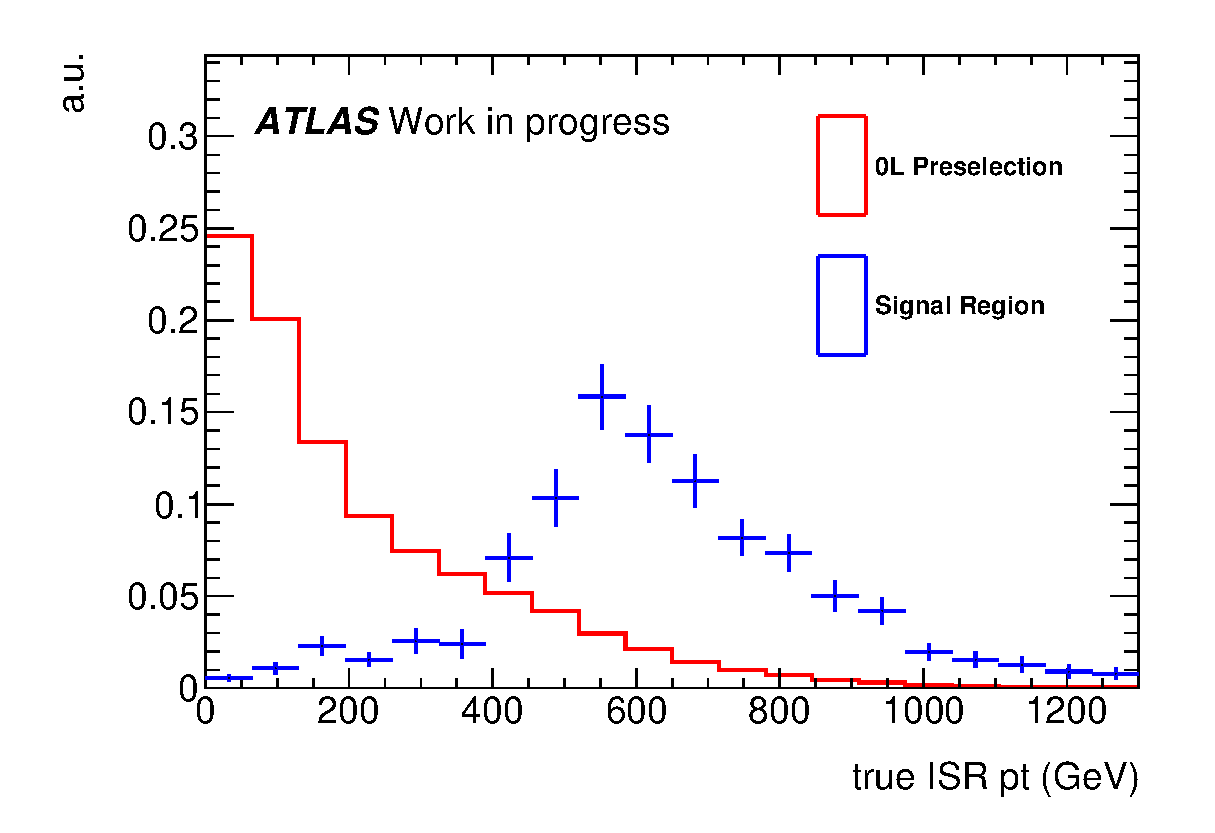
\includegraphics[width=0.80\textwidth]{./figures/strategy/Compare0L_truth.eps}
\caption[Distribution of true ISR $\pt$ for ttbar after the zero lepton preselection and after all signal region selections]{Distribution of true ISR $\pt$ for ttbar after the zero lepton preselection and after all signal region selections.  Both distributions have been normalized to unit area.}
\label{fig:ttbar:SR:trueISRpt_presel_SRC1}
\end{figure}

\indent A direct consequence of selecting for only strong ISR $\ttbar$ is that the predicted $\ttbar$ background rates in the signal region is directly related to the amount of ISR/FSR in the MC.  The next-to-leading order (NLO) \textsc{Powheg+\pythia6} $\ttbar$ MC has a $\sim30$ percent ISR/FSR systematic uncertainty in the high ISR $\pt$ region.  The ISR/FSR uncertainty would dominate the systematic uncertainty in this analysis if we relied on MC alone to predict the $\ttbar$ background in the signal region.  \\

\indent In order to decrease the ISR/FSR uncertainty, we directly measure the $\ttbar$ plus strong ISR rate in data using an one-lepton $\ttbar$ control region (CRTopC).  The ``lepton'' refers only to an electron or muon in this context because they can be reconstructed with much greater purity then taus.  The selections used to define the CRTopC is defined in table \ref{tab:ttbar1LepCRISR_def}. All variables used are defined in section \ref{Jigsaw:Variables}. \\

\begin{table}[h!]
  \begin{center}
    \def\arraystretch{1.4}%
    \begin{tabular}{c|c} \hline\hline
      {\bf Variable}     & 1 lepton $\ttbar$ control region \\ \hline \hline
      \multicolumn{2}{c}{1 Lepton Preselection}  \\ \hline
      $N_{lep}$  & 1                   \\
      \mtlepmet          & $<80\gev$           \\ 
      \mindrblep         & $<2.0$              \\ 
      \NjV               & $\ge5$              \\
      \NbV               & $\ge1$              \\
      \pTSFour           & $>40\gev$           \\
      \PTISR             & $\ge 400$           \\ \hline \hline
    \end{tabular}
  \caption{One-lepton $\ttbar$ control region (CRTopC) definitions. The one-lepton preselections defined in Table~\ref{tab:1Lcommon} are also applied. }
  \label{tab:ttbar1LepCRISR_def}
    \end{center}
\end{table}%

\indent In the one lepton CRTopC, the lepton is included as a ``jet'' in the Jigsaw ISR algorithm and will be counted as a sparticle jet or an ISR jet depending on which hemisphere it falls.  The lepton is meant to play the role of a hadronic tau jet in the zero-lepton signal region.  This approximation is justified since $\sim80$ percent of all $\ttbar$ events in the signal region decay via the hadronic tau channel.  \\

\indent CRTopC uses similar selections on the same kinematic variables as the signal region.  In this way, CRTopC captures the same kinematic features as the signal region by also targeting $\ttbar$ with high ISR $\pt$. Some signal region requirements such as the correlations on ISR and $\met$ are removed to increase statistics and lower signal contamination.  For example, the signal region $\dphiISRI > 3.0$ requirement is removed.  The $\dphiISRI$ variable specifies the direction of neutrino relative to the direction of the ISR.  A requirement of $\dphiISRI>3.0$ essentially selects specific alignments between the $\ttbar$ decay axis and the $\ttbar$ vs ISR boost axis.  Removing this requirement opens up more phase space for $\ttbar$ to decay but does not change the requirement on strong ISR $\pt$. \\

\indent The $\pTjV>50\gev$ cut is relaxed to $\pTjV>40\gev$ in order to increase statistics in the CR.  The $\pTjV$ cut specifies the $\pt$ of the 4th jet in the sparticle system.  The $\pTjV$ cut can be correlated with ISR/FSR because there is a chance that the 4th most energetic jet in the sparticle system is from radiation and not from a top decay.  However for this analysis it is more important to accurately gauge the amount of hard ISR of order hundred or more GeV that the $\ttbar$ system recoils against then amount of additional radiation in the same hemisphere as $\ttbar$. We found that loosening $\pTjV$ cut to 40 GeV does not result in a large difference in the true ISR $\pt$ distribution in the CRCTop and SR. \\

\indent  Stop signal, especially those with $\Delta m \neq m_{t}$, tend to produce more $\met$ because of the presence of neutralinos.  A $\mtlepmet$ less than $80\gev$ requirement is added to remove signal contamination.   A $\mindrblep$ less than $2.0$ requirement is also added to increase $\ttbar$ purity and ensure orthogonality to the $W$+jets control region. $\mtlepmet$ is defined in equation \ref{eqn:mtlep} and $\mindrblep$ is defined in equation \ref{eqn:mindrblep}. \\

\begin{equation}
\mtlepmet = (E_{T}^{lep}+\met)^{2}-({\vec {p}}_{T}^{lep}+{\vec {E}}_{T}^{miss})^{2} =m_{lep}^{2}+2(E_{T}^{lep}\met-{\vec {p}}_{T}^{lep}\cdot {\vec {E}}_{T}^{miss})
\label{eqn:mtlep}
\end{equation}

\begin{equation}
\mindrblep = \min_{jets~with~two~highest~b-tagging~value} \sqrt{ \Delta\eta(bjet, lep)^2 + \Delta\phi(bjet, lep)^2}
\label{eqn:mindrblep}
\end{equation}


\indent Figure \ref{fig:ttbar:CR:trueISRpt} shows the true ISR $\pt$ distribution for $\ttbar$ in the control region and the signal region.  Both distributions peak at roughly 550 $\gev$ and have similar shapes.  The one-lepton control region essentially measures the amount of $\ttbar$ plus strong ISR directly in data.  By normalizing $\ttbar$ background rates to the control region, we are able to limit the ISR/FSR uncertainty to below 10 percent for all $\RISR$ regions.  \\

\indent The close kinematic selection between the CRTopC and the signal region lowers many other systematics.   For example, the 6 percent uncertainty on jet energy scale and jet energy resolution can be partial attributed to the control region and the signal region having similar jet $\pt$ requirements. A more detailed discussion of systematics can be found in chapter \ref{chap:Uncertainties} \\

\begin{figure}[h!]
  \centering
	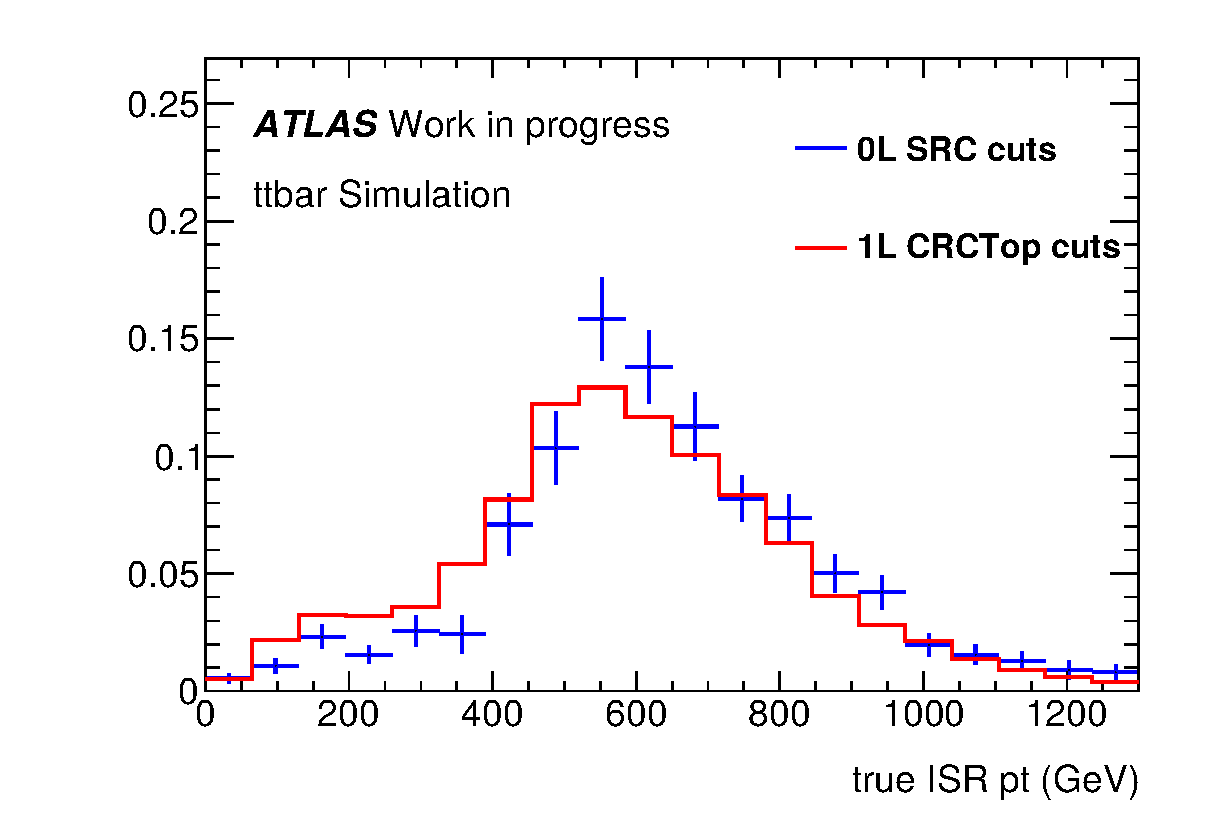
\includegraphics[width=0.65\textwidth]{./figures/ttbar/truePtISR_SRC_CRC_compare.eps}
	\caption[True ISR $\pt$ distribution for $\ttbar$ that after signal region and $\ttbar$ control region (CRTopC) selections]{True ISR $\pt$ distribution for $\ttbar$ that after signal region and $\ttbar$ control region (CRTopC) selections.  Both control and signal region distributions peak at roughly 550 $\gev$ demonstrating that the one-lepton control region and the zero-lepton signal region select for the same $\ttbar$ plus strong ISR events.  Therefore, the one-lepton control region is able to directly measure the amount of $\ttbar$ with high ISR $\pt$ directly from data.  This lets us predict the $\ttbar$ background rate in the signal region with minimal extrapolation between the control region and the signal region.}
	\label{fig:ttbar:CR:trueISRpt}
\end{figure}

\subsubsection{CRTopC Signal Contamination}

\indent Control regions are designed to have low expected signal rates.  If stop events are present in the control region then it can be misinterpreted as additional SM background.  In this way, a high expected signal rate in the control region decreases signal sensitivity.  The amount of signal contamination can be quantified as the signal over background ratio in the control region.  In general signal contamination should not exceed $\sim10$ percent in any control region.\\

\indent Signal contamination in CRTopC ranges from 1 percent at high stop masses to 12 percent at low stop masses for all stop masses that we are sensitive to and are not already excluded by previous stop experiments.  Signal contamination from stop masses that the analysis is not sensitive to are not important.  If the stop exists but has a mass that the analysis is not sensitive to, the stop will not be discovered regardless of the amount of signal contamination in the control region.\\

\indent The largest signal contamination occurs at a stop mass of 225 to 250 $\gev$.   Here, the signal contamination approaches 12 percent due to the large stop production cross section.  Lower stop masses result in higher signal contamination but our search does not have sensitivity to regions below 225 $\gev$.  \\

\indent The fact that CRTopC can attain such low signal contamination while selecting for $\ttbar$ background with close kinematic features to the signal region is impressive.  The signal region has a S/B ratio of approximately 2$\:$1 for stop masses between 250 $\gev$ and 400 $\gev$.   In comparison, CRTopC is able to achieve signal contamination of around 5 to 12 percent for the same stop masses.  \\

\indent CRCTop has a factor of 20-40 smaller S/B when compared to the signal region because of mainly two reasons.  First CRCTop is a one-lepton region while the signal region is a zero lepton region. \\

\indent The signal region primarily selects for stops that decay fully hadronically with a $\sim44$ percent branching fraction.  However, the $\ttbar$ background in the signal region mainly decay via the single hadronic tau decay channel with only a 10 percent decay fraction.  The signal region therefore gains a factor of five in S/B ratio because of the difference in stop and $\ttbar$ branching fractions.    \\

\indent Meanwhile, the one-lepton control region selects both stop signal and $\ttbar$ background primarily from the single muon and single electron decay channels.  Signal and background therefore has similar decay fractions in CRTopC.  This means CRTopC has a factor of five smaller S/B then the signal region simply because of branching fractions.  \\

\indent The signal region also gains S/B by requiring strong correlations between the ISR system and $\met$.  The signal region separates the signal and background into 5 bins in $\RISR$.  This targets the signal's peak in $\RISR$.  In contrast, CRTopC do not have separate $\RISR$ bins.  Integrating over all $\RISR$ instead of specifically targeting the bins under the signal region peak decreases the S/B by a factor of 2-5 depending on the stop mass and location of the signal $\RISR$ peak.  \\

\indent At the same time, removing the $\dphiISRI > 3.0$ requirement in the control region decreases S/B by another factor of 3.  Removing the requirements on the ISR and $\met$ correlations open up more phase space but do not change the requirement on strong $\ttbar$ ISR $\pt$.  \\

\indent These factors combine to make up the factor of $\sim40$ decrease in the S/B between the signal region and the CRTopC; all the while preserving the agreement in the true $\ttbar$ ISR $\pt$ distribution shown in Figure \ref{fig:ttbar:CR:trueISRpt}. \\

\subsubsection{$\ttbar$ Control Region Yields and Distributions}

\indent Distribution of important variables after a background-only fit to $\intlumi$ $\ifb$ of data are shown for CRTopC in Figure \ref{fig:CRTopC}.   There is a noticeable trend in the data over MC comparison in the CRTopC $\pTISR$ distribution.  The disagreement is not surprising given that a priori we have a 30 percent uncertainty due to the ISR/FSR uncertainty.  This further demonstrate the need for a control region that directly measures the amount of $\ttbar$ with strong ISR using data. \\

\indent The fitted normalization scale factor for $\ttbar$ is 0.707. This scale factor is quiet different from 1.0 which indicates that the $\ttbar$ MC does a poor job of modeling the high ISR $\pt$ phase space.  Again, this difference is not unexpected given the 30 percent ISR/FSR uncertainty on $\ttbar$ MC in this high ISR $\pt$ region.  \\

\begin{figure}[h!]
  \centering
    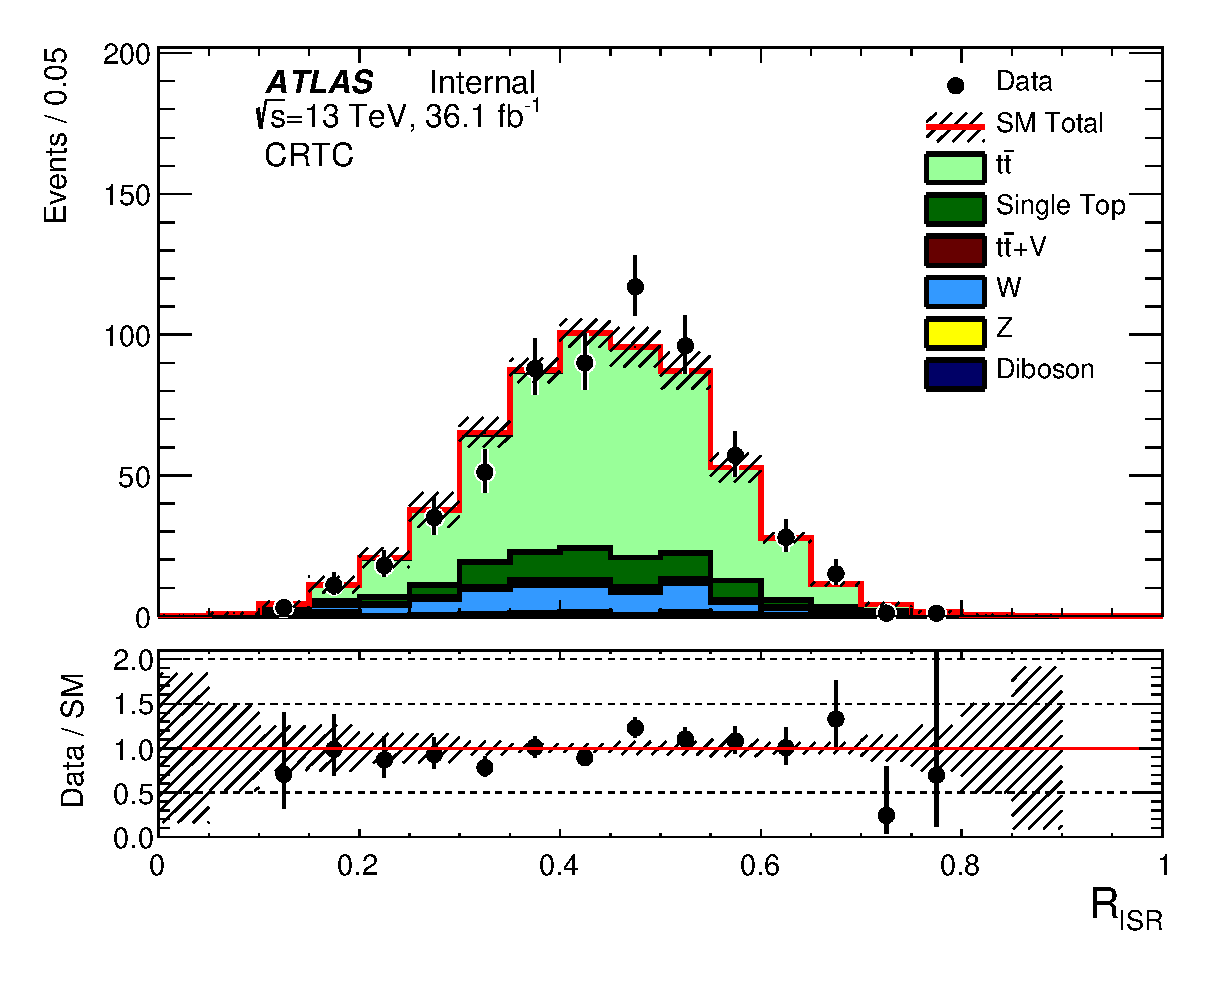
\includegraphics[width=0.45\textwidth]{figures/ttbar/postfit/CA_RISR_CRTopC}
    \includegraphics[width=0.45\textwidth]{figures/ttbar/postfit/CA_pTISR_CRTopC}
    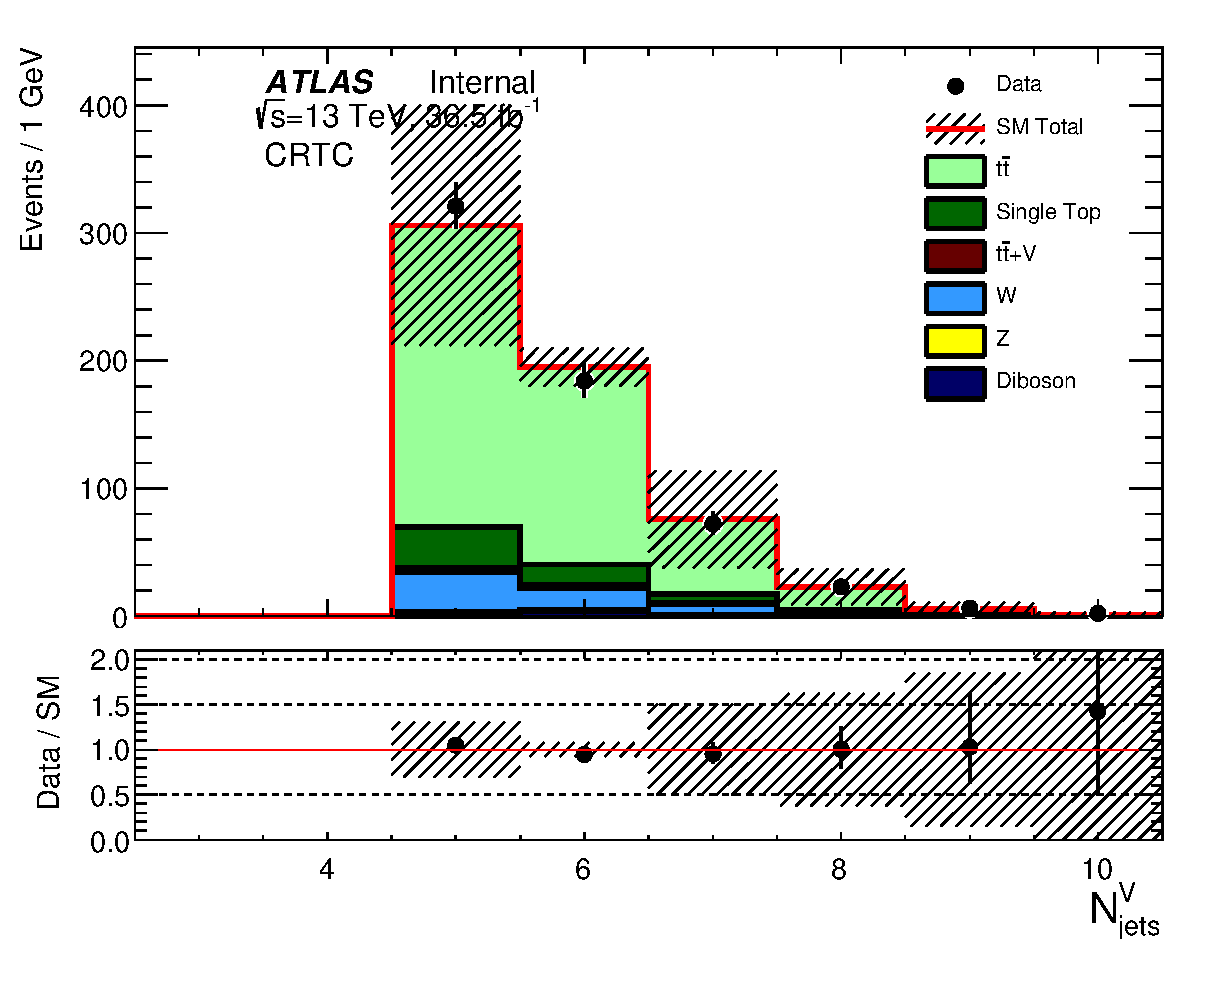
\includegraphics[width=0.45\textwidth]{figures/ttbar/postfit/CA_NjV_CRTopC}
    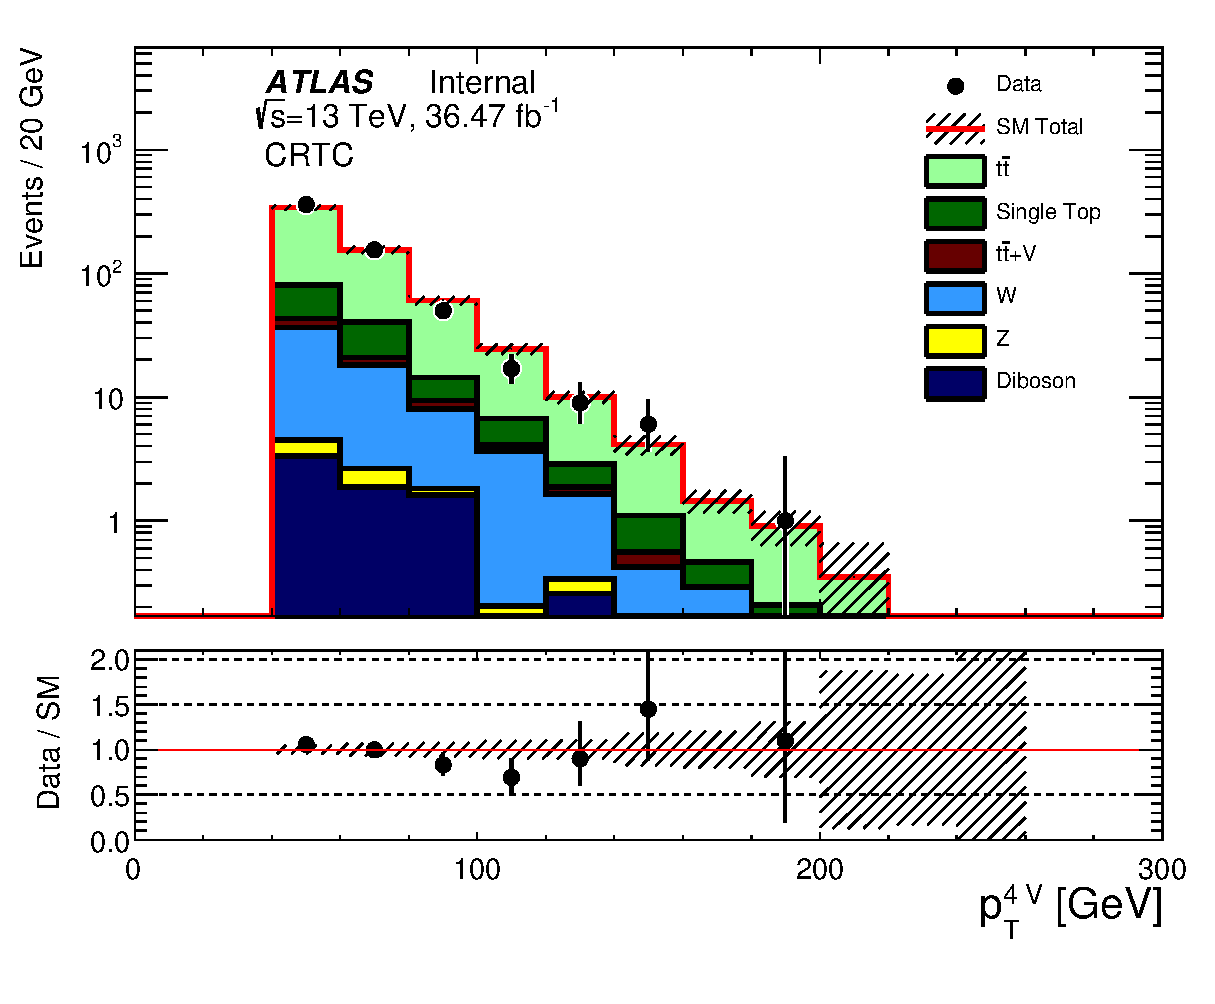
\includegraphics[width=0.45\textwidth]{figures/ttbar/postfit/CA_pTjV4_CRTopC_log}
    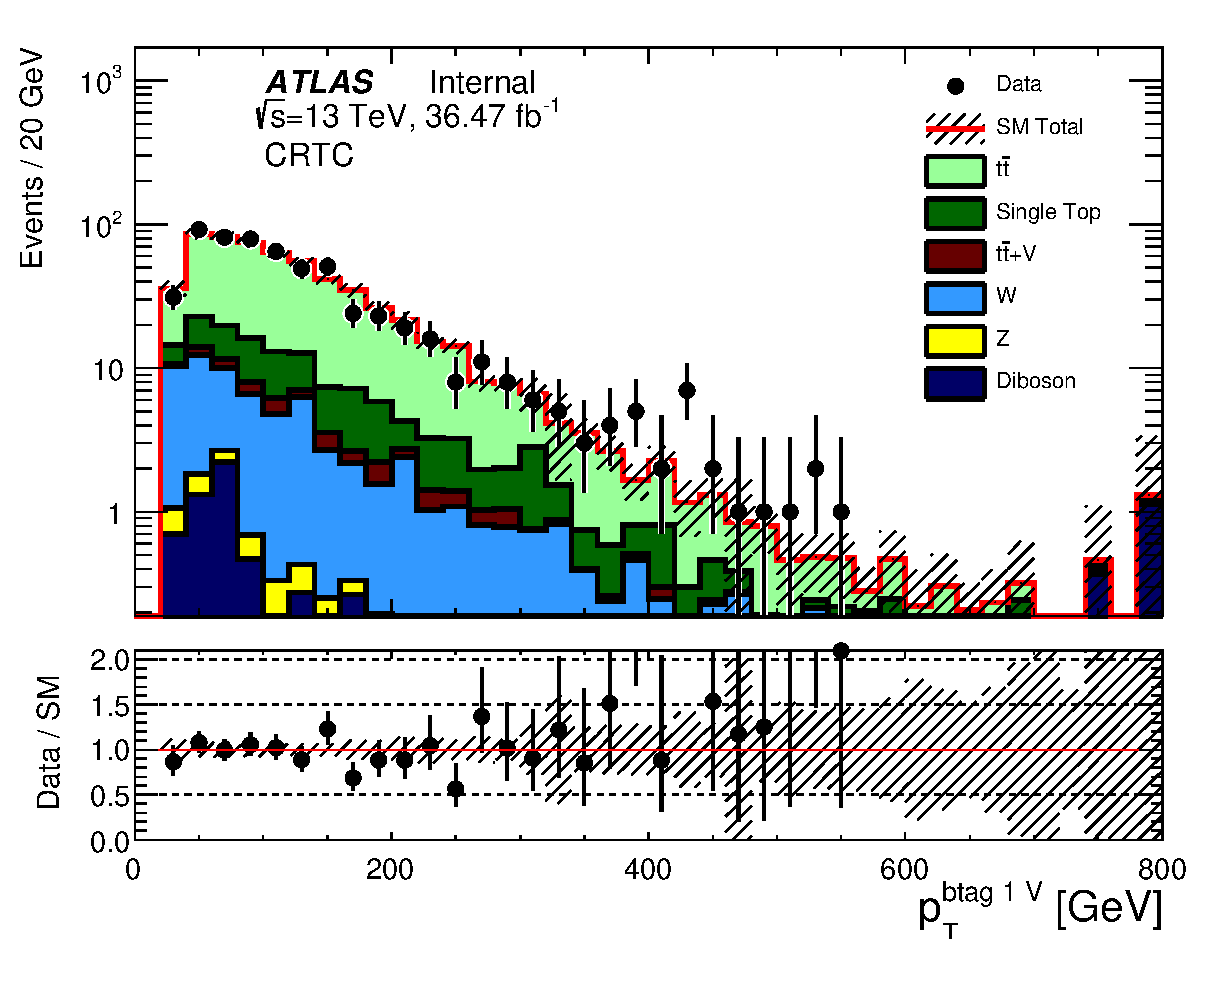
\includegraphics[width=0.45\textwidth]{figures/ttbar/postfit/CA_pTbV1_CRTopC_log}
    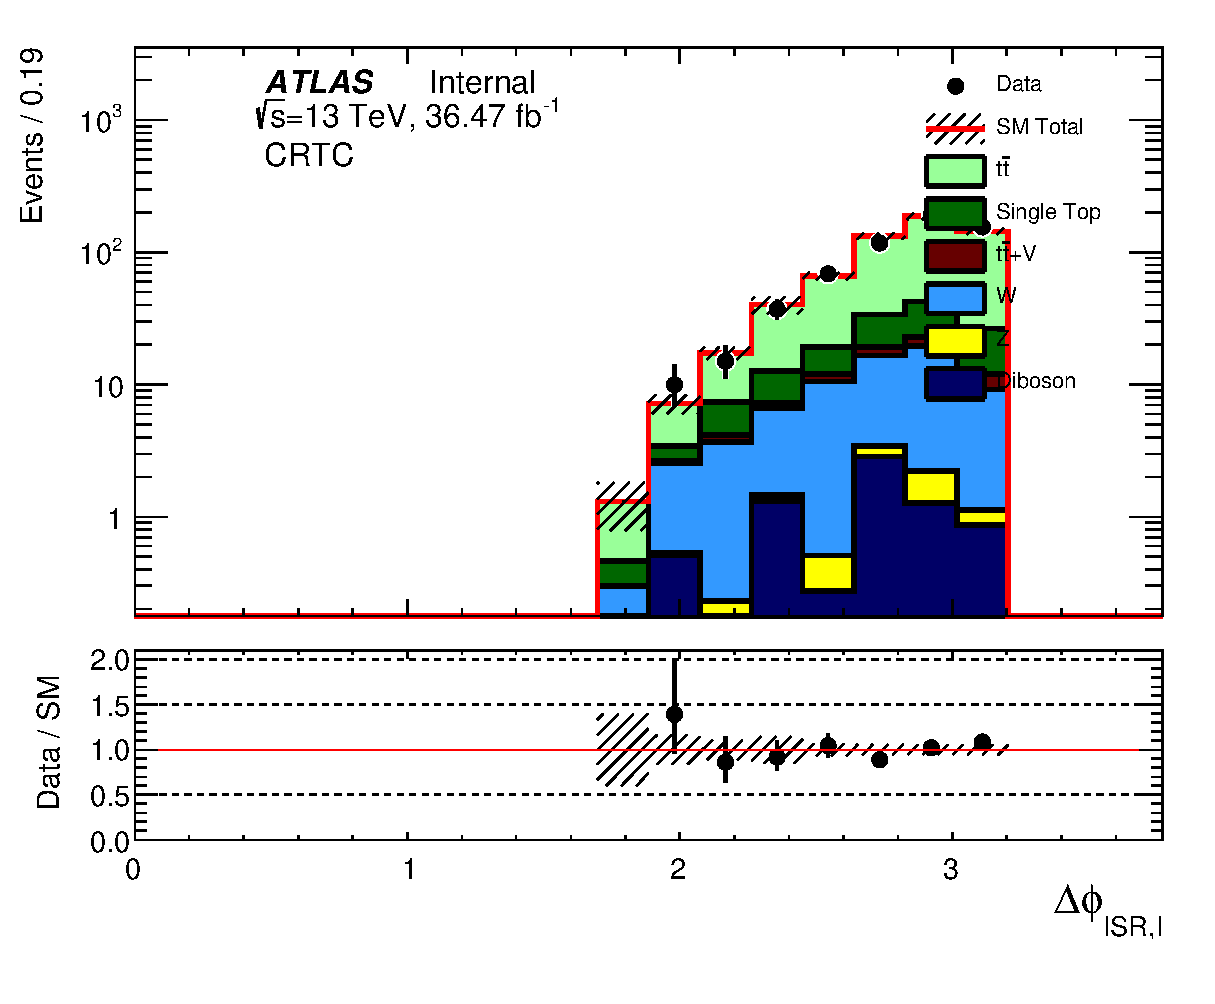
\includegraphics[width=0.45\textwidth]{figures/ttbar/postfit/CA_dphiISRI_CRTopC_log}
   \caption[One-lepton $\ttbar$ control region (CRTopC) distributions for $\intlumi$ $\ifb$ of data]{One-lepton $\ttbar$ control region (CRCTop) distributions for $\intlumi$ $\ifb$ of data. All backgrounds yields have already been normalized to data by performing a background only fit.  The ratio between data and MC is shown in the bottom panel. The hashed area in both the top and lower panel represent the uncertainty due to MC statistics and detector systematic uncertainties.}
  \label{fig:CRTopC}
\end{figure}

\indent There seem to be no significant slope in the data over MC comparison in the CRCTop $\pTjV$ distribution.  This is further evidence that the extrapolation from 40 to 50 GeV across $\pTjV$ is allowed.  No strong trends outside of statistical and systematic uncertainties are observed for any other distributions. \\

\indent CRTopC yields from before and after the background only fit can be found in Table \ref{table.bkgonly.CRTopC}



\begin{table}[h!]
\begin{center}
\setlength{\tabcolsep}{0.0pc}
{\small
%%
\begin{tabular*}{\textwidth}{@{\extracolsep{\fill}}lr}
\noalign{\smallskip}\hline\noalign{\smallskip}
{\bf Yields}           & CRTopC                  \\[-0.05cm]
\noalign{\smallskip}\hline\noalign{\smallskip}
%%
Observed data events          & $611$                       \\
\noalign{\smallskip}\hline\noalign{\smallskip}
%%
Fitted SM bkg events         & $610.96 \pm 24.72$                     \\
\noalign{\smallskip}\hline\noalign{\smallskip}
%%
        Fitted $\ttbar$ events         & $461.47 \pm 31.85$                 \\
%%
        Fitted Wjets events         & $64.94 \pm 12.12$                    \\
%%
        Fitted Zjets events         & $2.15 \pm 0.90$                \\
%%
        Fitted TtbarV events         & $11.32 \pm 2.19$                    \\
%%
        Fitted SingleTop events         & $63.49 \pm 20.36$                   \\
%%
        Fitted Diboson events         & $7.58 \pm 2.84$                       \\
%%
        Fitted Multijets events         & $0.00 \pm 0.00$                    \\
%%     
 \noalign{\smallskip}\hline\noalign{\smallskip}
%%
MC exp. SM events              & $777.01 \pm 14.91$                   \\
\noalign{\smallskip}\hline\noalign{\smallskip}
%%
        MC exp. $\ttbar$ events         & $652.93 \pm 7.35$                     \\
%%
        MC exp. Wjets events         & $51.34 \pm 6.02$                 \\
%%
        MC exp. Zjets events         & $1.84 \pm 0.58$                 \\
%%
        MC exp. TtbarV events         & $8.78 \pm 0.90$                      \\
%%
        MC exp. SingleTop events         & $54.53 \pm 5.03$                  \\
%%
        MC exp. Diboson events         & $7.58 \pm 2.87$                     \\
%%
        MC exp. Multijets events         & $0.00 \pm 0.00$                   \\
%%     \\
\noalign{\smallskip}\hline\noalign{\smallskip}
Fitted $\ttbar$ normalization scale factor & $0.707 \pm 0.050$ \\
\noalign{\smallskip}\hline\noalign{\smallskip}
\end{tabular*}
%%%
}
\caption[CRTopC MC Yield and background-only fit results for $\intlumi$ $\ifb$ of data]{CRTopC MC Yield and background-only fit results for $\intlumi$ $\ifb$ of data. MC exp. events are expected background rates directly from MC predictions.  Fitted background event rates are the expected background rates after normalizing the MC to data by simultaneously fitting all control regions using a background only fit.  The fitted $\ttbar$ normalization scale factor is equal to (Fitted $\ttbar$ events)/(MC exp. $\ttbar$ events). The quoted uncertainties include statistical and systematic uncertainties. }
\label{table.bkgonly.CRTopC}
\end{center}
\end{table}
%

\subsection{Validating $\ttbar$ Predictions in Signal Region using a Zero Lepton Validation Region}
\label{sec:Bkg:ttbar:VR}

\indent We also define a zero-lepton $\ttbar$ validation region to validate the predicted background rates in the signal region.  The $\ttbar$ validation region (VRTopC) is kinematically similar but completely orthogonal to the signal region.  Plus the validation region must have limited signal contamination and high $\ttbar$ purity. \\

\indent The $\dphiISRI > 3.0$ selection in the signal region is inverted in the validation region to limit signal contamination. In signal, the neutralinos and the ISR tend to be back-to-back in $\phi$.  The neutralinos gain most of their momenta by recoiling against ISR and the correlation is strong. \\

\indent In contrast, $\dphiISRI$ has a different physical interpretation in SM $\ttbar$ events.   In $\ttbar$ events, $\dphiISRI$ specifies the neutrino direction relative to the direction of the ISR.  Inverting the $\dphiISRI$ selection selects for $\ttbar$ events with a different decay axis relative to $\ttbar$ vs ISR boost axis but does not change the requirements on strong ISR $\pt$.  \\

\indent For this reason, the $\dphiISRI < 3.0$ requirement in the validation region rejects $\sim50$ percent of signal events while retaining $\sim80$ percent of background. \\

\indent The requirement on $\MS$ is reduced in the validation region to 100 $\GeV$ (vs. 300 $\GeV$ in the signal) and the $\NjV$ selection is relaxed to $\ge 4$ (vs. $\NjV \ge 5$ in the signal region).  Relaxing both requirements enhances the background yields in the validation region. \\

\indent Similar to CRTopC, the $\pTjV>50\gev$ selection is also relaxed to $\pTjV>40\gev$ to increase the validation region statistics. \\

\indent Finally, a requirement of $\MV/\MS < 0.6$ is added to reduce signal contamination and reject QCD multijet background. \\


\begin{table}
  \begin{center}
    \def\arraystretch{1.4}%
    \begin{tabular}{c||c} \hline\hline
      {\bf Variable} & 0 leption $\ttbar$ validation region \\ \hline \hline
      \NjV           & $\ge4$                \\
      \NbV           & $\ge1$                \\
      \pTbV          & $\ge 40$              \\
      \PTISR         & $\ge 400$             \\
      \MS            & $>100\gev$            \\
      $\MV/\MS$      & $<0.6$                \\
      \dphiISRI      & $<3.00$               \\ \hline \hline
    \end{tabular}
  \caption{Zero-lepton $\ttbar$+ISR validation region definitions, in addition
    to the SRC requirements listed in Table~\ref{tab:1Lcommon}.}
  \end{center}
  \label{tab:ttbar0LepVR}
\end{table}%

\indent The distributions of select variables in VRTopC are shown in Figure \ref{fig:ttbar0Lep1bVRISR}.  The background rates have been normalized to control regions through the use of a background only fit to $\intlumi$ $\ifb$ of data. \\

\begin{figure}[htbp]
  \centering
    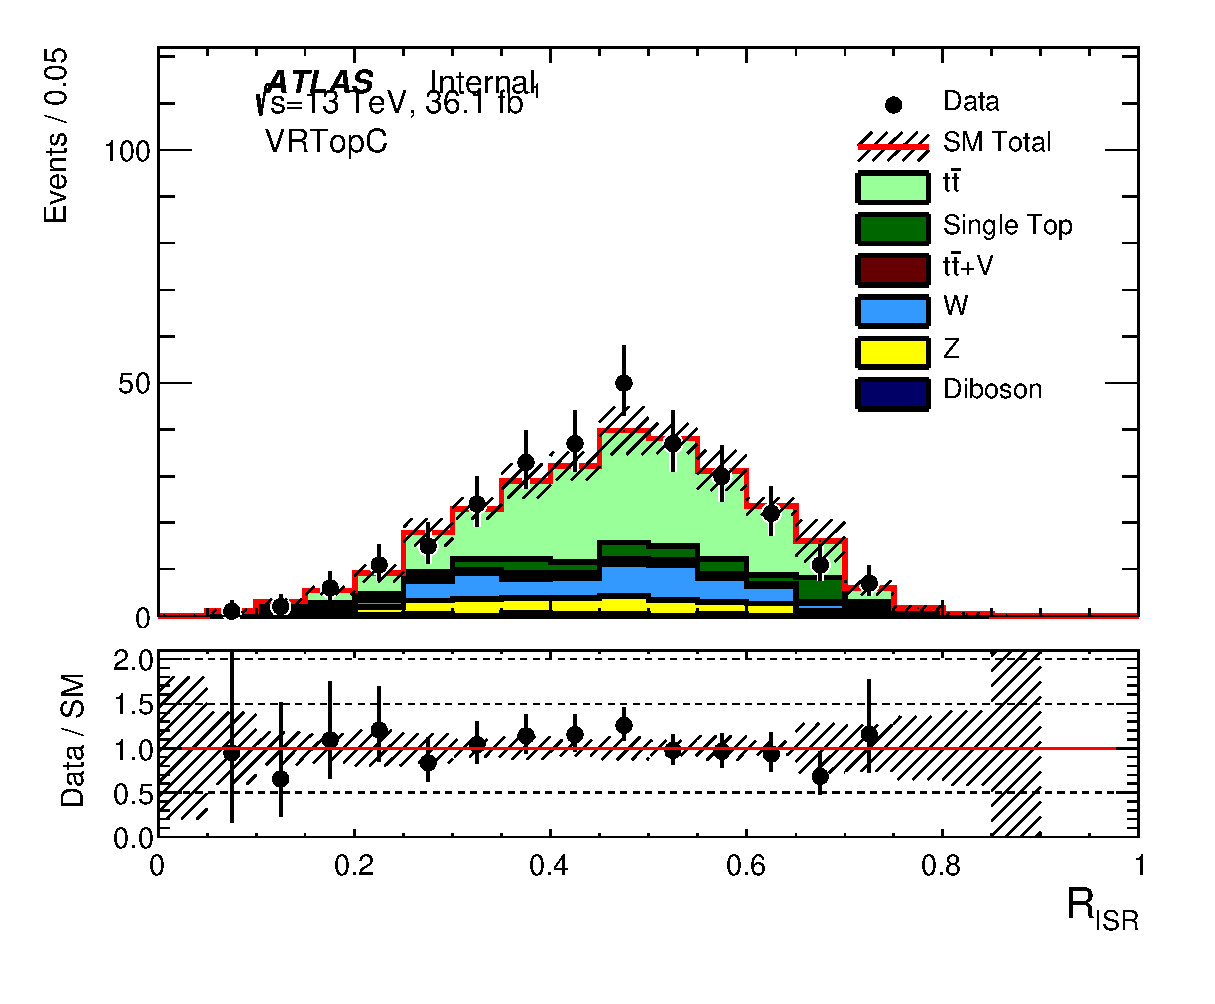
\includegraphics[width=0.45\textwidth]{figures/ttbar/postfit/CA_RISR_VRTopC}
    \includegraphics[width=0.45\textwidth]{figures/ttbar/postfit/CA_pTISR_VRTopC}
    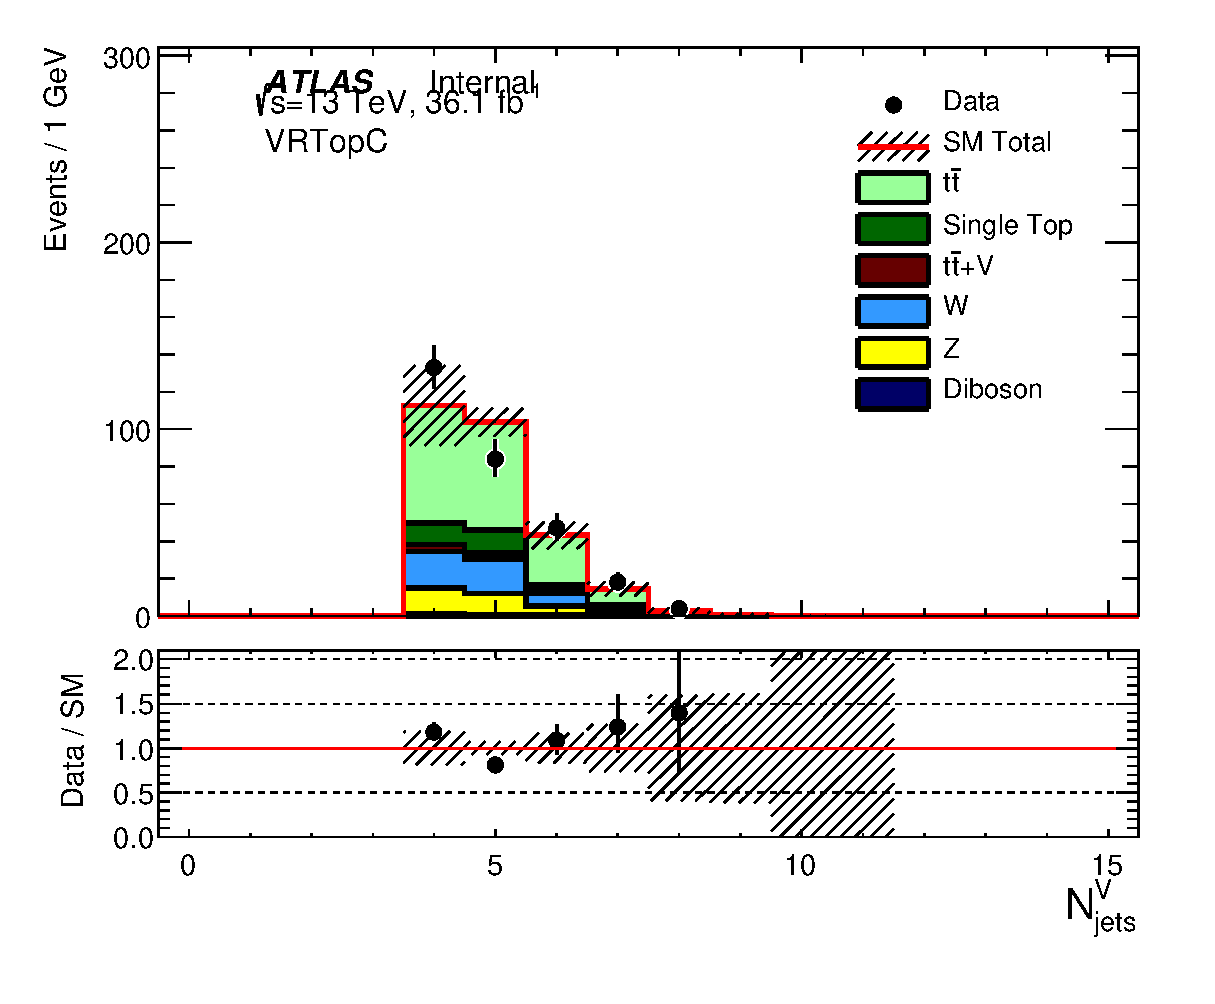
\includegraphics[width=0.45\textwidth]{figures/ttbar/postfit/CA_NjV_VRTopC}
    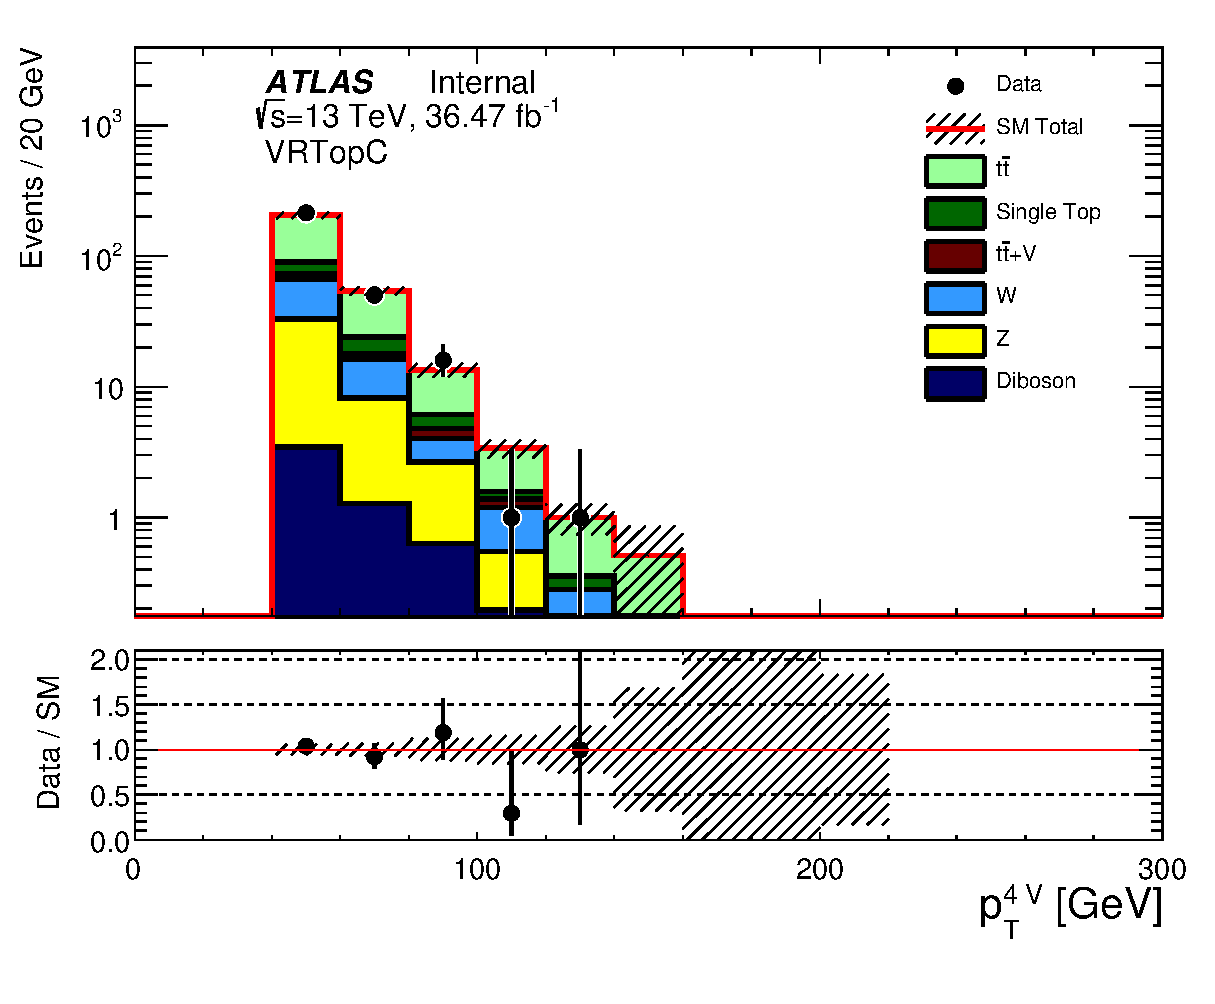
\includegraphics[width=0.45\textwidth]{figures/ttbar/postfit/CA_pTjV4_VRTopC_log}
    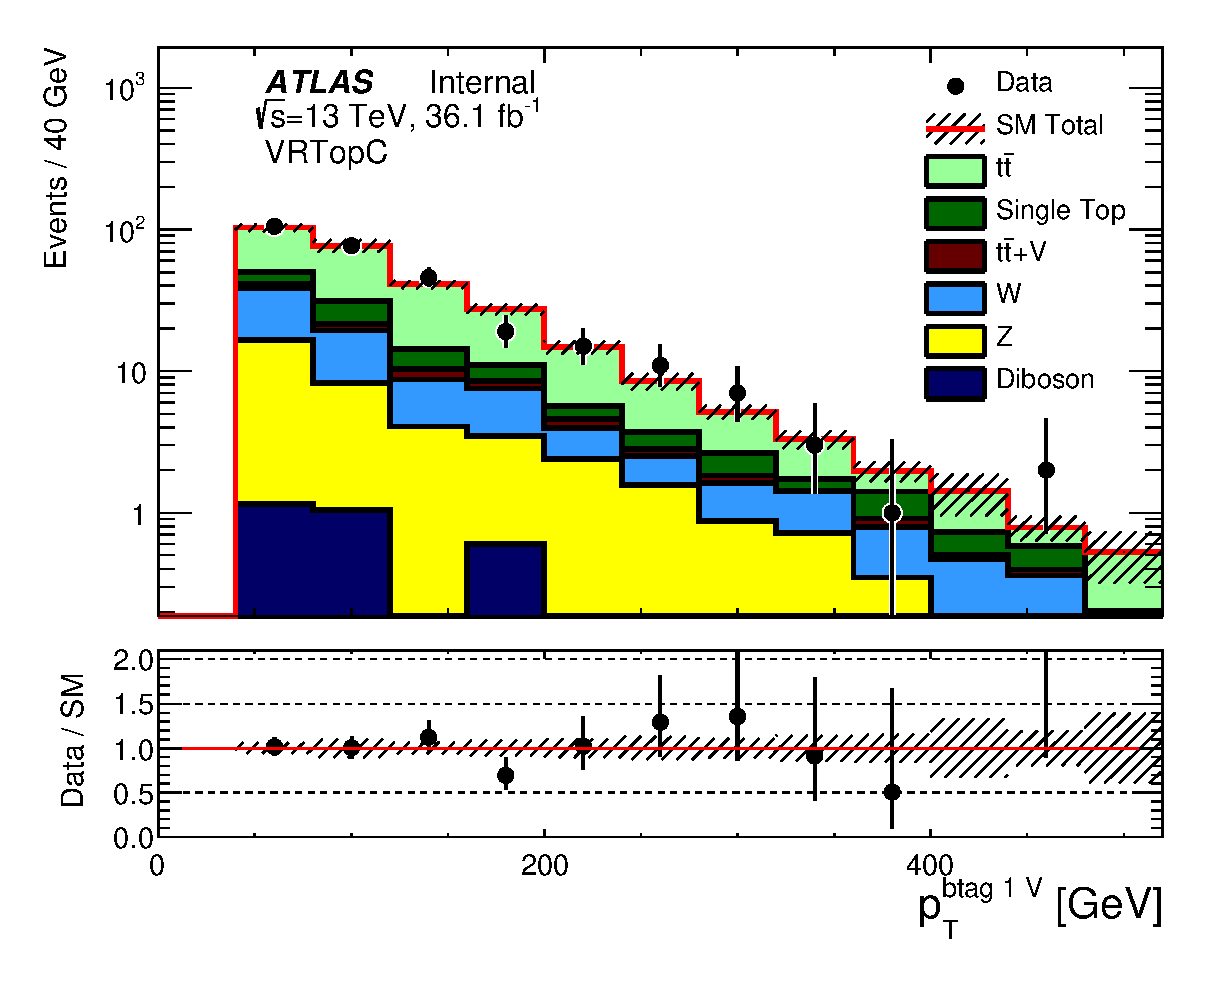
\includegraphics[width=0.45\textwidth]{figures/ttbar/postfit/CA_pTbV1_VRTopC_log}
        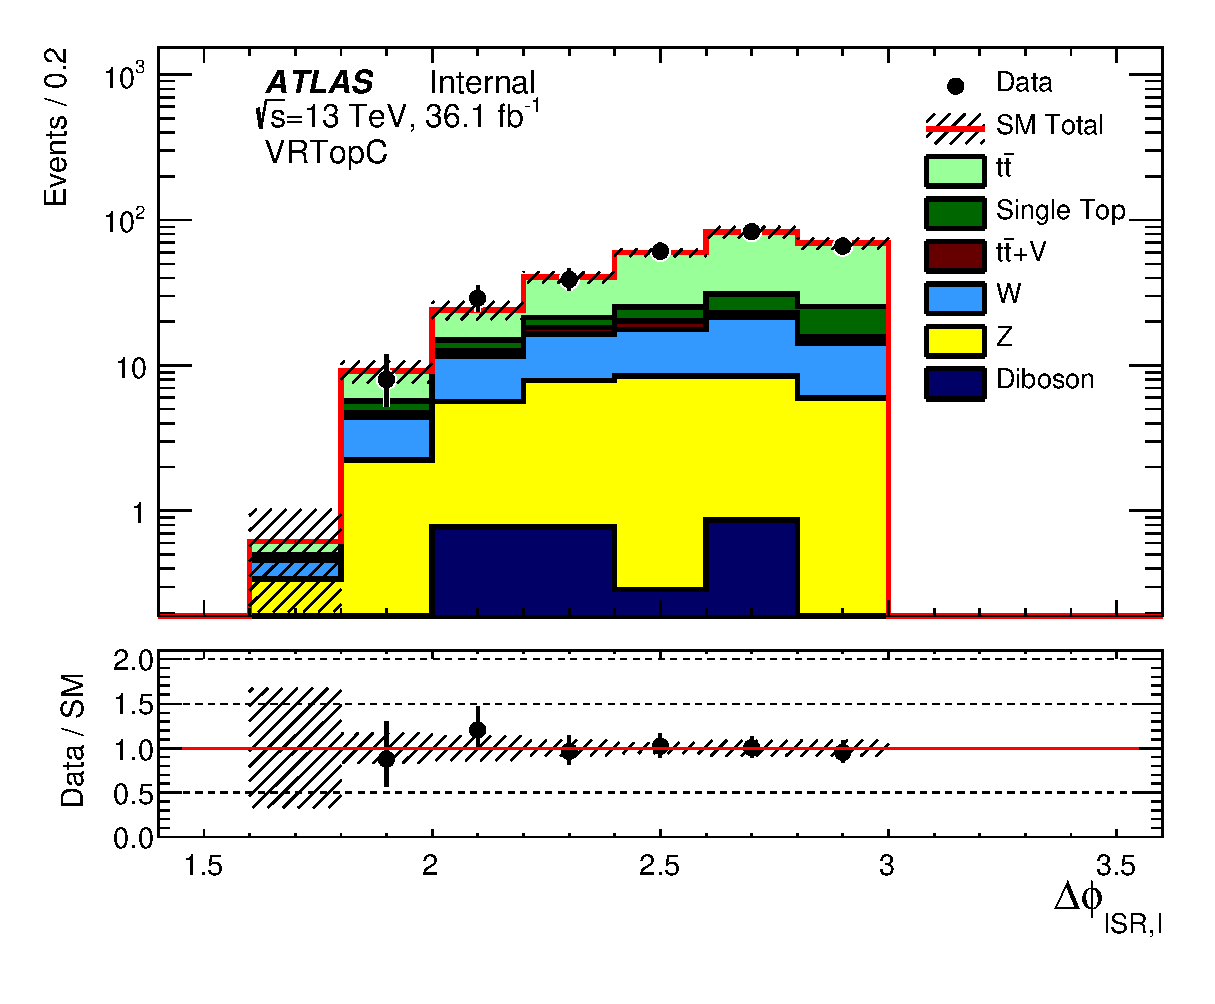
\includegraphics[width=0.45\textwidth]{figures/ttbar/postfit/CA_dphiISRI_VRTopC_log}
  \caption[Distribution of select variables in the zero lepton $\ttbar$ validation region]{Distribution of select variables in the zero lepton $\ttbar$ validation region.  The ratio between data and MC predictions are shown in the bottom panel.  The background rates have been normalized to control regions through the use of a background only fit to $\intlumi$ $\ifb$ of data.  Experimental systematic uncertainties on background predictions are depicted as the hashed bands. }
\label{fig:ttbar0Lep1bVRISR}
\end{figure}

\indent The predicted background rate in the VRTopC agrees with data to within $1\sigma$.  This demonstrates that CRTopC is an effective predictor of $\ttbar$ background rates in the validation region and the signal region.  The $\RISR$ shape is well modeled as we see no distinct trends in the data vs MC ratio in $\RISR$. \\

\indent Similar to CRTopC, there is a noticeable trend in the data over MC comparison in the VRTopC $\pTISR$ distribution.  Again this is expected because the MC has a $\sim30$ percent ISR/FSR uncertainties in the high ISR $\pt$ region and is a poor predictor of ISR $\pt$ rates.  \\

\indent The MC and data yields in VRTopC is given in table \ref{table.bkgonly.VRTopC}.  The background MCs have already been normalized to their respective control regions using a background only fit.  The validation region has the $0.707 \pm 0.050$ $\ttbar$ normalization scale factor applied to its expected $\ttbar$ MC rates.  The fact that data in VRTopC agrees with the post-fit predicted background rate is evidence that CRTopC can predict the background rate in the signal region by effectively measuring the amount of $\ttbar$ with at least 400 $\gev$ of ISR $\pt$ directly from data.    \\



\begin{table} [h!]
\begin{center}
\setlength{\tabcolsep}{0.0pc}
{\small
%%
\begin{tabular*}{\textwidth}{@{\extracolsep{\fill}}lr}
\noalign{\smallskip}\hline\noalign{\smallskip}
{\bf VRTop yields}           & VRTopC               \\[-0.05cm]
\noalign{\smallskip}\hline\noalign{\smallskip}
%%
Observed events          & $286$                            \\
\noalign{\smallskip}\hline\noalign{\smallskip}
%%
Fitted bkg events         & $289.20 \pm 34.10$                   \\
\noalign{\smallskip}\hline\noalign{\smallskip}
%%
        Fitted TTbar events         & $162.19 \pm 18.77$                   \\
%%
        Fitted Wjets events         & $47.37 \pm 10.17$                    \\
%%
        Fitted Zjets events         & $36.13 \pm 10.26$                   \\
%%
        Fitted TtbarV events         & $8.89 \pm 1.68$                   \\
%%
        Fitted SingleTop events         & $28.67_{-28.67}^{+30.30}$                      \\
%%
        Fitted Diboson events         & $3.00 \pm 1.86$                       \\
%%
        Fitted Multijets events         & $2.96 \pm 2.33$                      \\
%%     
 \noalign{\smallskip}\hline\noalign{\smallskip}
%%
MC exp. SM events              & $335.18 \pm 31.37$                     \\
\noalign{\smallskip}\hline\noalign{\smallskip}
%%
        MC exp. TTbar events         & $229.37 \pm 19.56$                   \\
%%
        MC exp. Wjets events         & $37.46 \pm 5.92$                      \\
%%
        MC exp. Zjets events         & $30.88 \pm 4.18$                   \\
%%
        MC exp. TtbarV events         & $6.90 \pm 1.16$                 \\
%%
        MC exp. SingleTop events         & $24.60 \pm 24.60$                     \\
%%
        MC exp. Diboson events         & $3.01 \pm 1.88$                     \\
%%
        MC exp. Multijets events         & $2.96 \pm 2.33$                 \\
%%     \\
\noalign{\smallskip}\hline\noalign{\smallskip}
Fitted \ttbar normalization scale factor & $0.707 \pm 0.050$ \\
\noalign{\smallskip}\hline\noalign{\smallskip}
\end{tabular*}
%%%
}
\end{center}
\caption[VRTopC expected background and data yields with $\intlumi$ $\ifb$ of data]{VRTopC expected background and data yields with $\intlumi$ $\ifb$ of data. MC exp. events are expected background rates directly from MC predictions.  Fitted background events correspond to the expected background rates after simultaneously fitting all control regions using a background only fit.  The backgrounds are normalized to the data in control regions and the fitted $\ttbar$ normalization scale factor derived from the fit is $0.707\pm0.050$.  The fitted normalization scale factors are then applied to the expected MC yields giving the fitted expected background rate.  The agreement between the fitted expected background yield and data in VRTopC is evidence that CRTopC is correctly measuring the amount of $\ttbar$ with high ISR $\pt$.  The quoted uncertainties include statistical and systematic uncertainties. }
\label{table.bkgonly.VRTopC}
\end{table}
%

%\indent This agreement both in magnitude and shape demonstrates two things.  One, the $\ttbar$ control region indeed does correctly measure the amount of $\ttbar$ plus strong ISR that exists in both signal and validation region.  Two, the subdominant background predictions also cannot by wrong by more than around 100 percent.  For example we clearly would see disagreement in between data vs MC in this VR if the MC underestimated W+jets or Z+jets background by 100 percent.  Both of these facts give us confidence that the background prediction in the signal region is correct. \\

\section{Subdominant Backgrounds}
\label{sec:Bkg:sub}

\subsection{Standard Model W+Jets}
\label{sec:Bkg:wjet}

\indent A $W$ boson produced in conjunction with QCD jets ($W$+jets) is our largest subdominant background.  $W$+jets comprises 9 percent of the total background in the signal region.  However the distribution of $W$+jets is not uniform across $\RISR$.  $W$+jets can reach 20-25 percent of all backgrounds in signal region bins with the largest $\RISR$.  This means the $W$+jets contribution mostly affects high stop mass samples because those signal samples peak at high $\RISR$. \\

\indent We estimate $W$+jets using an one lepton control region defined in table \ref{tab:WJetCR}..  The one lepton $W$+jet control region is designed to ensure high $W$+jet purity.   All one lepton control regions are mutually exclusive including the ttbar, $W$+jets and single top control region. \\

\begin{table}[h!]
  \begin{center}
    \begin{tabular}{c||c}
      \hline \hline
          {\bf Variables }                           & $W$+jets control region                \\ \hline \hline
      Number of leptons             & 1                                          \\ 
      Number of jets (incl. lepton) & $\geq 4$                                     \\ 
      $\pt$ of jets (incl. lepton)  & (80,80,40,40) GeV                            \\ 
      \mindphijettwomet             & $> 0.4$                                      \\ 
      $\met$                        & $>250$ GeV                                   \\ 
      \mtlepmet                     & ($>30, <100$ GeV) \\ 
      Number of $b$-jets            & $=1$                            \\ 
      \mantikttwelvezero            & $<60\,$GeV         \\ 
      \mindrblep                    & $>2.0$             \\ \hline \hline
    \end{tabular}
  \end{center}
  \caption{Summary of the selection for the one lepton $W$+jets control region.}
  \label{tab:WJetCR}
\end{table}

\indent The lepton is treated as a jet for the jet multiplicity and the jet $\pt$ requirements.  Similar to the one lepton $\ttbar$ control region, the lepton is meant to play the role of a hadronic tau jet in the zero-lepton signal region.  \\

\indent $\mtlepmet$ is defined in equation \ref{eqn:mtlep} as the transverse mass of the lepton and the $\met$.  The $\mtlepmet$ selection ensures that the transverse mass is consistent with those originating from a $W$ boson.  \\

\indent Orthogonality between the $W$+jet control region and the single top control region is ensured by the requirement on the number of $b$-jets.  Orthogonality between $\ttbar$ control region and $W$+jet control region is ensured by the selection on $\mindrblep$.  $\mindrblep$ is defined in equation \ref{eqn:mindrblep} as the minimum $\Delta R$ between the two jets with the highest b-tag value and the selected lepton. \\

\indent $\mantikttwelvezero$ is defined as the mass of an $\antikt$ jet built with a distance parameter of $R=1.2$ instead of regular $R=0.4$.  The $\antikt$ algorithm clusters calorimeter energy into a jet according to the distance metric $R$ and is covered in detail in section \ref{sec:jet:reco}.  The $\antikt$ algorithm will form a perfectly conical jet of radius $R$ if no other hard objects are found within a cone of $2R$.  If two hard objects exist within $R<\Delta R<2R$ of one another then two jets will be formed splitting the energy cells between them.  \\

\indent The large R=1.2 jet is designed to cluster all the energy of a boosted top quark into a single jet.  If the jet contains a boosted top, the invariant mass of jet should be close to $\sim m_t$. The $\mantikttwelvezero < 60 \gev$ is designed to reject events with reconstructed boosted tops.  \\

\indent  Distributions of select kinematic variables in the $\Wjets$ control region are shown in Figure ~\ref{fig:CRWpts}.  The MC background has been normalized to data by performing a simultaneous fit to all control regions.  The hashed bands on the total SM background correspond to the total experimental systematical uncertainty plus the MC statistical uncertainty.  The yield in the $\Wjets$ control region is given in Table~\ref{table.bkgonly.CRW}.  \\

\indent  The fitted $W$+jets normalization scale factor is $1.27 \pm 0.15$.  Data and MC are compatible to within statistical uncertainty.  No strong trends are observed in the data to MC ratios in any of the distributions. \\

\begin{figure}[!h]
  \centering
  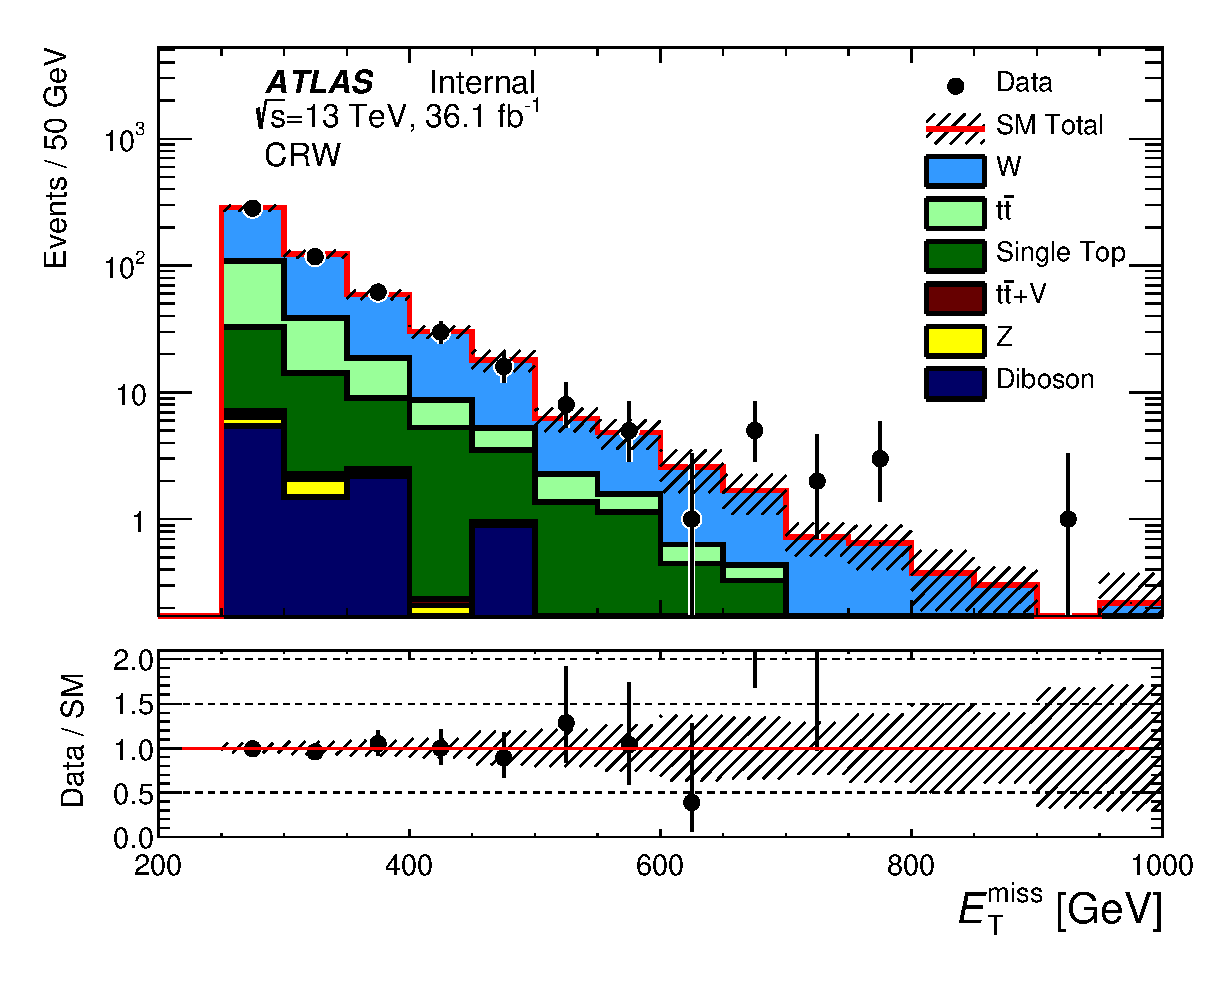
\includegraphics[width=0.45\textwidth]{figures/wJets/postfit/Met_CRW_log.eps}
    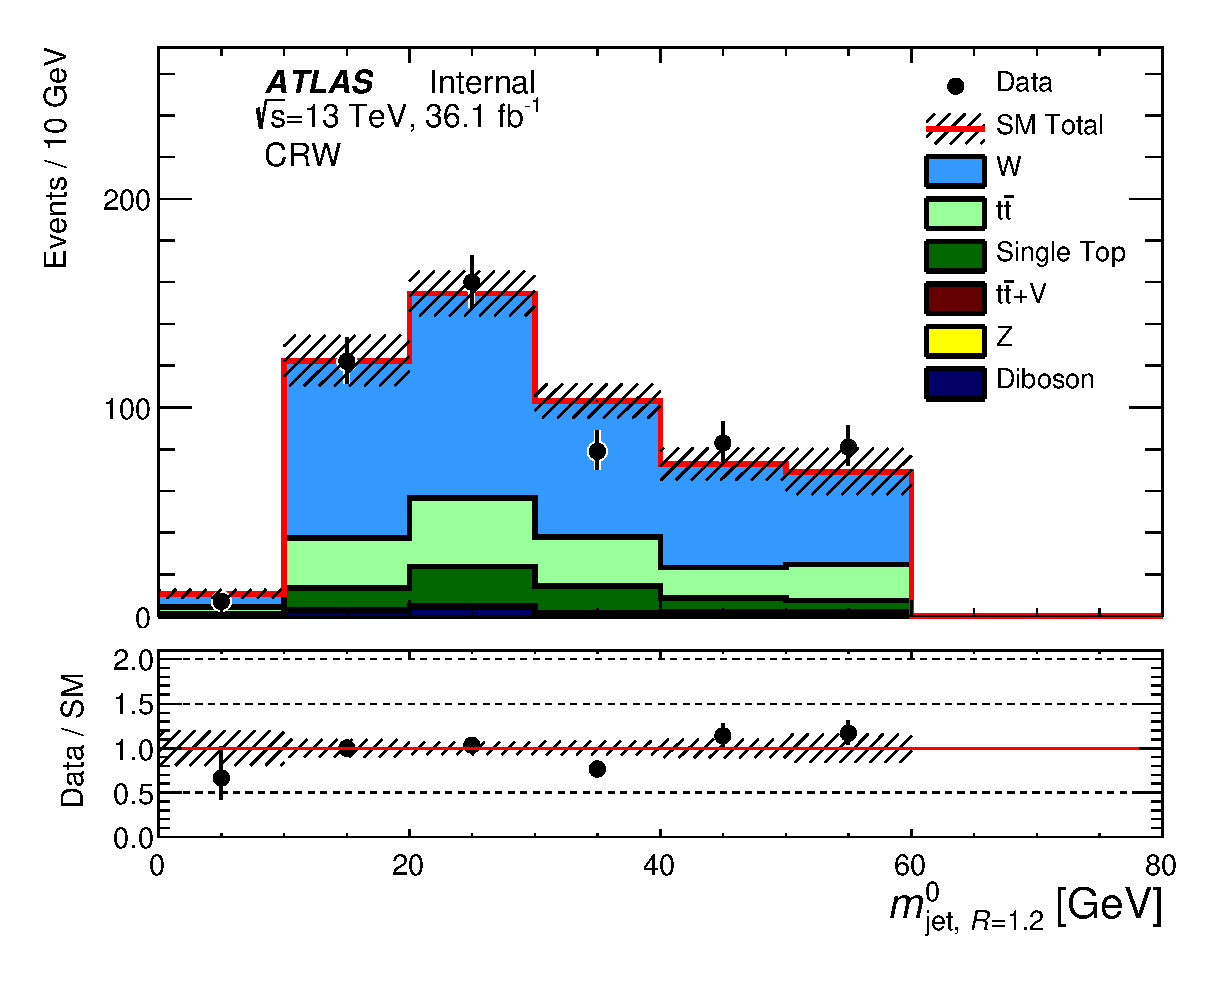
\includegraphics[width=0.45\textwidth]{figures/wJets/postfit/AntiKt12M_0__CRW.eps}
  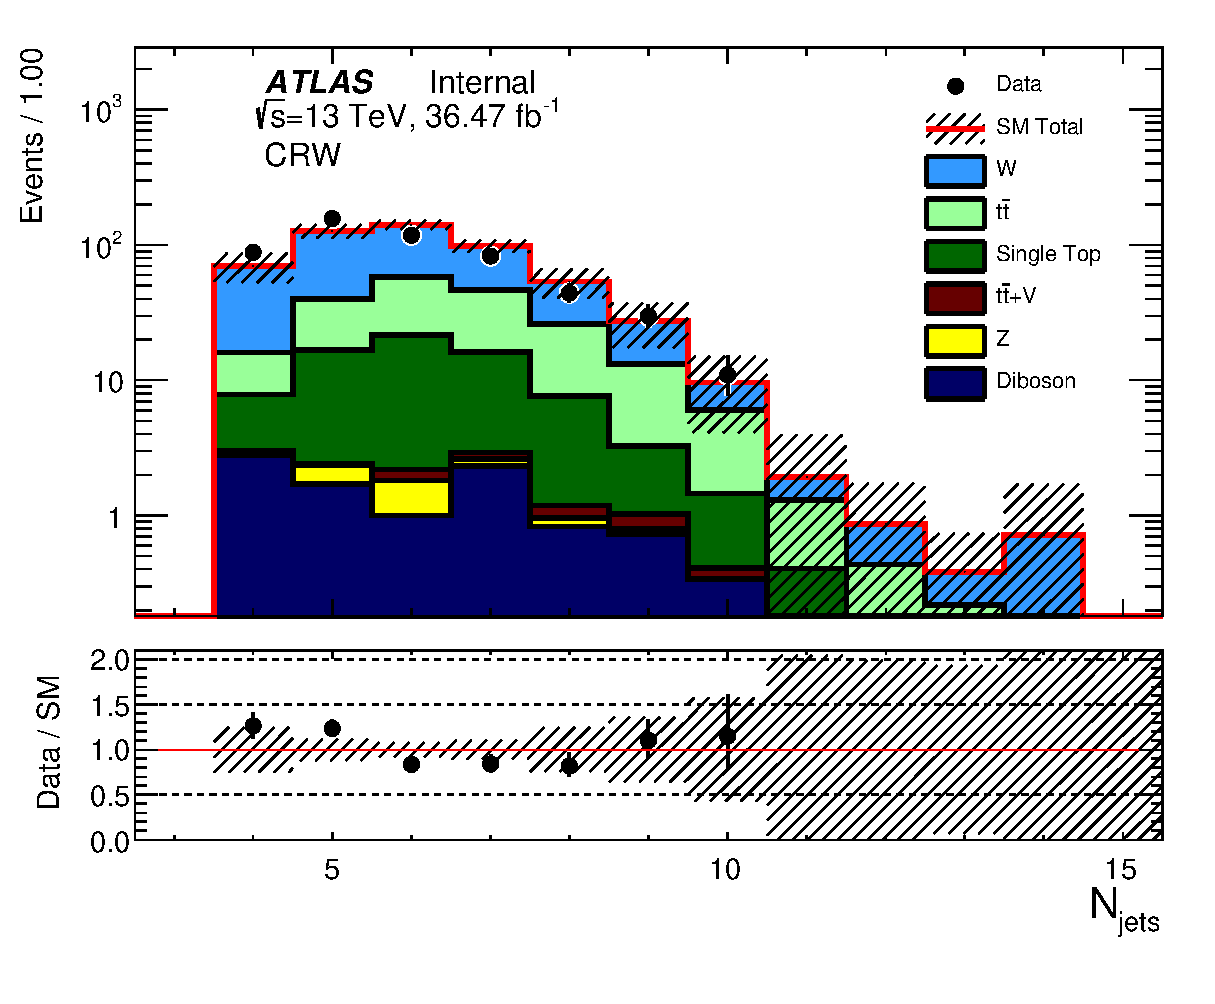
\includegraphics[width=0.45\textwidth]{figures/wJets/postfit/NJets_CRW_log.eps}
  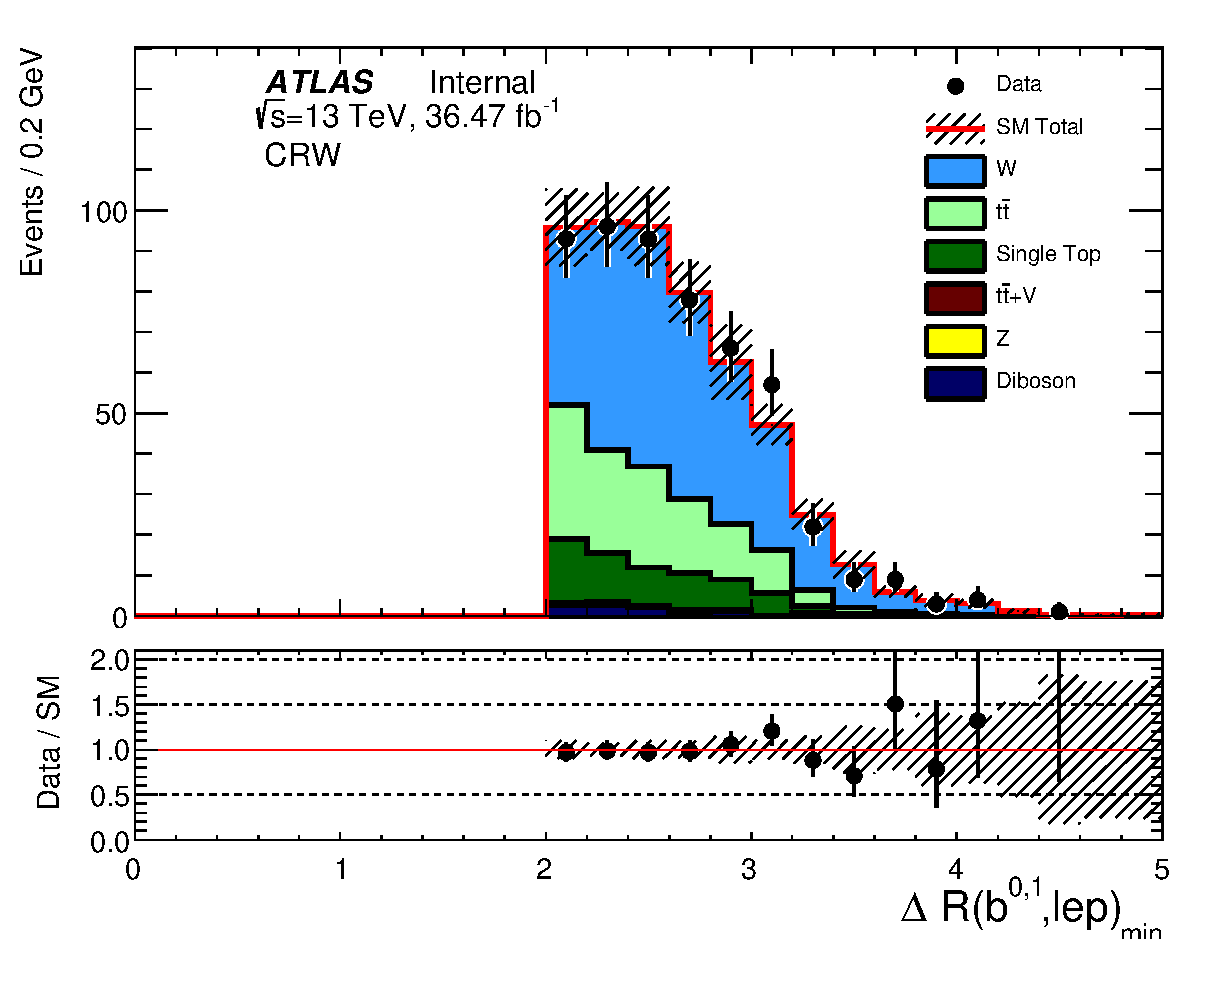
\includegraphics[width=0.45\textwidth]{figures/wJets/postfit/MinDRBLep_CRW.eps}]
  \caption[Kinematic distributions in the $\Wjets$ control region after the background only fit to $\intlumi$ $\ifb$ of data]{Kinematic distributions in the $\Wjets$ control region after the background only fit to $\intlumi$ $\ifb$ of data. From left to right and top to bottom, the variables shown are $\met$, $\mtlepmet$, $\mantikttwelvezero$ and the number of jets and $\mindrblep$. The expected SM background has been normalized to the data by performing a simultaneous fit to all control regions.  The hatched band on the total SM background correspond to the total experimental systematic uncertainty plus the MC statistical uncertainty.}
  \label{fig:CRWpts}
\end{figure}



\begin{table}[h!]
\caption[$W$+jets control region MC Yield and background-only fit results for $\intlumi$ $\ifb$ of data]{$W$+jets control region MC Yield and background-only fit results for $\intlumi$ $\ifb$ of data. MC exp. events are expected background rates directly from MC predictions.  Fitted background event rates are the expected background rates after normalizing the MC to data by simultaneously fitting all control regions using a background only fit.  The fitted $W$+jets normalization scale factor is equal to (Fitted $\Wjets$ events)/(MC exp. $\Wjets$ events). The quoted uncertainties include statistical and systematic uncertainties. }
\label{table.bkgonly.CRW}
\begin{center}
\setlength{\tabcolsep}{0.0pc}
{\small
%%
\begin{tabular*}{\textwidth}{@{\extracolsep{\fill}}lr}
\noalign{\smallskip}\hline\noalign{\smallskip}
{\bf CRW yields}           & CRW                      \\[-0.05cm]
\noalign{\smallskip}\hline\noalign{\smallskip}
%%
Observed events          & $533$                       \\
\noalign{\smallskip}\hline\noalign{\smallskip}
%%
Fitted bkg events         & $533.23 \pm 23.09$                 \\
\noalign{\smallskip}\hline\noalign{\smallskip}
%%
        Fitted TTbar events         & $115.60 \pm 18.76$                     \\
%%
        Fitted Wjets events         & $349.54 \pm 38.87$                  \\
%%
        Fitted Zjets events         & $1.86 \pm 0.63$                   \\
%%
        Fitted TtbarV events         & $1.15 \pm 0.43$                     \\
%%
        Fitted SingleTop events         & $54.76 \pm 20.41$                     \\
%%
        Fitted Diboson events         & $10.31 \pm 2.34$                    \\
%%
        Fitted Multijets events         & $0.00 \pm 0.00$                 \\
%%     
 \noalign{\smallskip}\hline\noalign{\smallskip}
%%
MC exp. SM events              & $458.28 \pm 21.31$                     \\
\noalign{\smallskip}\hline\noalign{\smallskip}
%%
        MC exp. TTbar events         & $122.28 \pm 15.29$                   \\
%%
        MC exp. Wjets events         & $276.00 \pm 5.53$             \\
%%
        MC exp. Zjets events         & $1.79 \pm 0.52$                     \\
%%
        MC exp. TtbarV events         & $0.89 \pm 0.35$                      \\
%%
        MC exp. SingleTop events         & $47.00 \pm 5.70$                   \\
%%
        MC exp. Diboson events         & $10.31 \pm 2.35$                   \\
%%
        MC exp. Multijets events         & $0.00 \pm 0.00$                \\
%%     \\
\noalign{\smallskip}\hline\noalign{\smallskip}
Fitted $W$+jets normalization scale factor & $1.27 \pm 0.15$ \\
\noalign{\smallskip}\hline\noalign{\smallskip}
\end{tabular*}
%%%
}
\end{center}
\end{table}
%

%\begin{table}[!h]
%  \centering
%  \begin{tabular}{c|c}
\hline\hline
\multicolumn{2}{c}{\bf CRW (60\% purity)} \\ \hline 
Z & 1.99 $\pm$ 0.45 \\
dibosons & 9.85 $\pm$ 1.76 \\
ttbar & 128.42 $\pm$ 3.82 \\
singleTop & 51.14 $\pm$ 3.37 \\
ttV & 1.07 $\pm$ 0.16 \\
W & 288.12 $\pm$ 8.86 \\
\hline
Total MC & 480.58 $\pm$ 10.38 \\
Data & 531.00 $\pm$ 23.04 \\
 \hline
SF & 1.17 $\pm$ 0.10 \\
\hline\hline
\end{tabular}

%  \caption{Yields in the $\Wjets$ CR with \intlumi\ \ifb\ of data.  }
%  \label{tab:CRW_yields}
%\end{table}


\subsection{Standard Model Single-Top}
\label{sec:Bkg:SingleTop}

\indent Standard Model single-top consists of 6\% of the total background in the signal region.  This rate varies between 2-9\% for any one signal region $\RISR$ bin.  A one lepton single-top control region is defined in Table \ref{tab:ST1LCR}.  The single-top control region is orthogonal to both the one lepton $W$+jets control region and $\ttbar$ control region.  \\

\begin{table}[h!]
  \begin{center}
    \begin{tabular}{c|c}
      \hline \hline
       { \bf Variables } & Single-top 1 lepton control region           \\ \hline
      Number of leptons             & 1                                            \\ 
      Number of jets (incl. lepton) & $\geq 4$                                     \\ 
      $\pt$ of jets (incl. lepton)  & (80,80,40,40) GeV                            \\ 
      \mindphijettwomet             & $> 0.4$                                      \\ \
      $\met$                        & $>250$ GeV                                   \\ \hline
      \mtlepmet                     & $>30$,$<100$ GeV \\ 
      Number of $b$-jets            & $\ge2$                          \\ 
      \mantikttwelvezero            & v$>120$ GeV       \\
      \mtbmin                       & $>200\,$GeV   \\ 
      \mindrblep                    & $>2.0$             \\ 
      \drbjetbjet                   & $>1.5$               \\ \hline \hline
    \end{tabular}
  \end{center}
  \caption{Selection for the one lepton single-top control region.  The one lepton preselection defined in Table \ref{tab:1Lcommon} is also applied.}
  \label{tab:ST1LCR}
\end{table}

\indent The lepton is treated as a jet for the jet multiplicity and the jet $\pt$ requirements as well as for the top reconstruction.  Similar to the one lepton $\ttbar$ control region, the lepton is meant to play the role of a hadronic tau jet in the zero-lepton signal region. \\

\indent $\mtlepmet$ is defined in equation \ref{eqn:mtlep} as the transverse mass of the lepton and the $\met$.  The $\mtlepmet$ selection ensures that the transverse mass is consistent with a $W$ decay.  \\

\indent The $\drbjetbjet$ variable is defined in equation \ref{eqn:drbb} as the $\Delta R$ between the two b-jets with the highest b-tagging values.  $\drbjetbjet > 1.5$ isolates single-top events and rejects $\ttbar$.  This gives the single-top control region a purity of $\sim50\%$. \\

\begin{equation}
\mindrblep = \sqrt{ \Delta\eta(b_1, b_2)^2 + \Delta\phi(b_1, b_2)^2}
\label{eqn:drbb}
\end{equation}

\indent The $\mantikttwelvezero > 120 \gev$ requirement selects for events with reconstructed boosted tops and ensures orthogonality with the $\Wjets$ control region.  $\mantikttwelvezero$ is defined as the mass of an $\antikt$ jet built with a distance parameter of $R=1.2$ instead of regular $R=0.4$.  The $\antikt$ algorithm clusters calorimeter energy into a jet according to the distance metric $R$ and is covered in detail in section \ref{sec:jet:reco}.  The large $R=1.2$ jet is designed to cluster all the energy of a boosted top quark into a single jet.  If the jet contains a boosted top, the invariant mass of jet should be close to $\sim m_t$.  \\

\indent $\mindrblep$ is defined in equation \ref{eqn:mindrblep} as the minimum $\Delta R$ between the two jets with the highest b-tag value and the selected lepton.  The $\mindrblep$ selection ensures orthogonality with the $\ttbar$ control region.  \\

\indent Kinematic distributions in the single control region are shown in Figure \ref{fig:CRST} and \ref{fig:CRST1}.  The MC background has been normalized to data by performing a simultaneous fit to all control regions.  The hashed bands on the total SM background correspond to the total experimental systematical uncertainty plus the MC statistical uncertainty.  The yield in the single-top control region is given in table~\ref{table.bkgonly.CRST}.  \\

\indent  Data and MC are compatible to within statistical uncertainty.  No strong trends are observed in the data to MC ratios in any of the distribution. \\

%\begin{table}[!htb]
%  \centering
%  \begin{tabular}{c|c}
\hline\hline
\multicolumn{2}{c}{\bf CRST (44\% purity)} \\ \hline 
Z & 0.11 $\pm$ 0.05 \\
dibosons & 1.52 $\pm$ 0.54 \\
ttbar & 34.17 $\pm$ 2.10 \\
singleTop & 45.62 $\pm$ 1.41 \\
ttV & 2.42 $\pm$ 0.19 \\
W & 19.72 $\pm$ 1.69 \\
\hline
Total MC & 103.57 $\pm$ 3.10 \\
Data & 113.00 $\pm$ 10.63 \\
 \hline
SF & 1.21 $\pm$ 0.29 \\
\hline\hline
\end{tabular}

%  \caption{Yields in the CRST in $\intlumi$ $\ifb$ of data.  }
%  \label{tab:CRST}
%\end{table}

\pagebreak
 
\begin{figure}[h!]
\begin{center}
      \begin{subfigure}[b]{0.40\textwidth}    
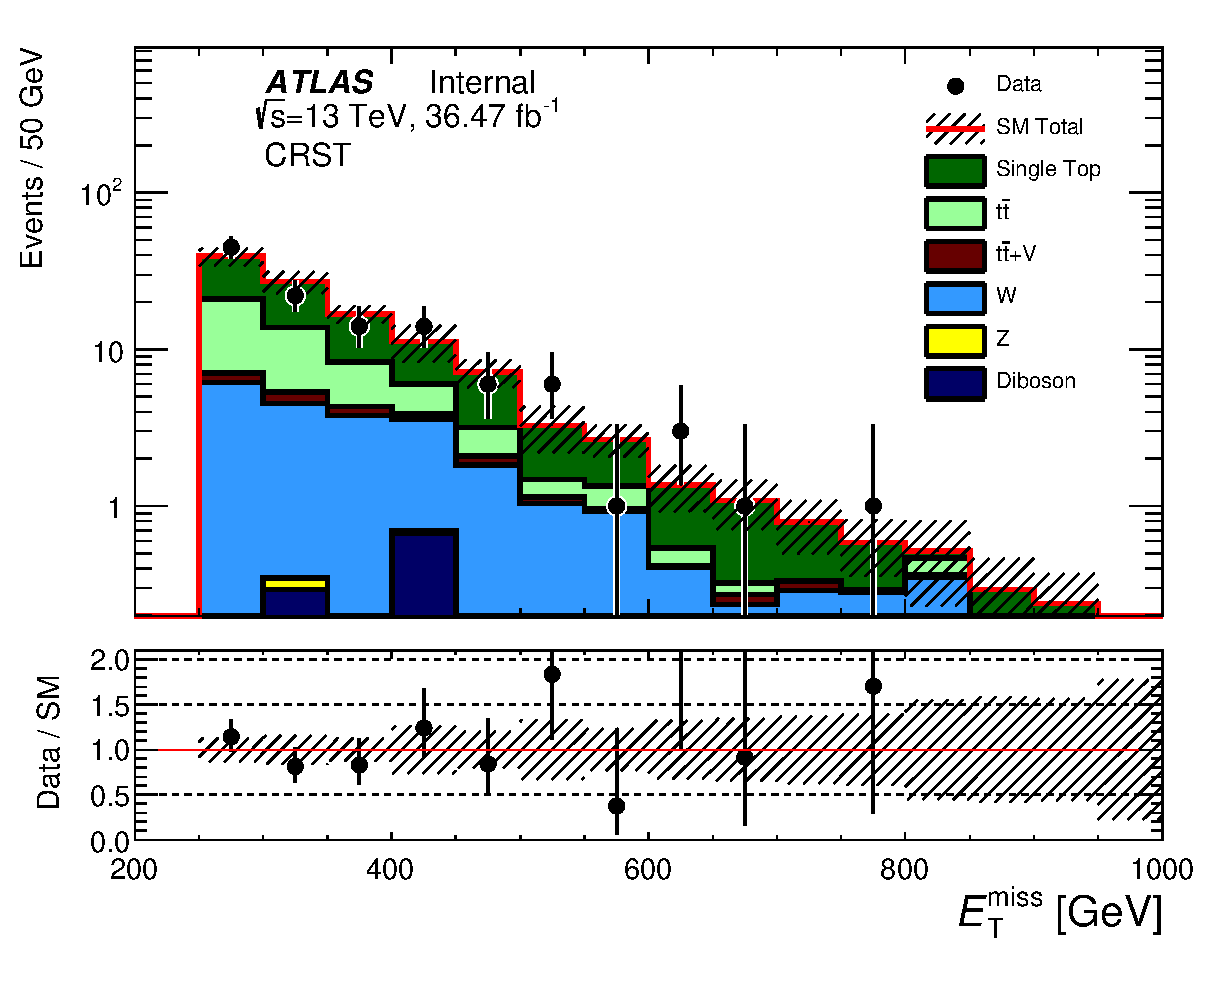
\includegraphics[width=\textwidth]{figures/singleTop/postfit/Met_CRST_log.eps}
                 \caption{ }
    \end{subfigure}
     \begin{subfigure}[b]{0.40\textwidth}    
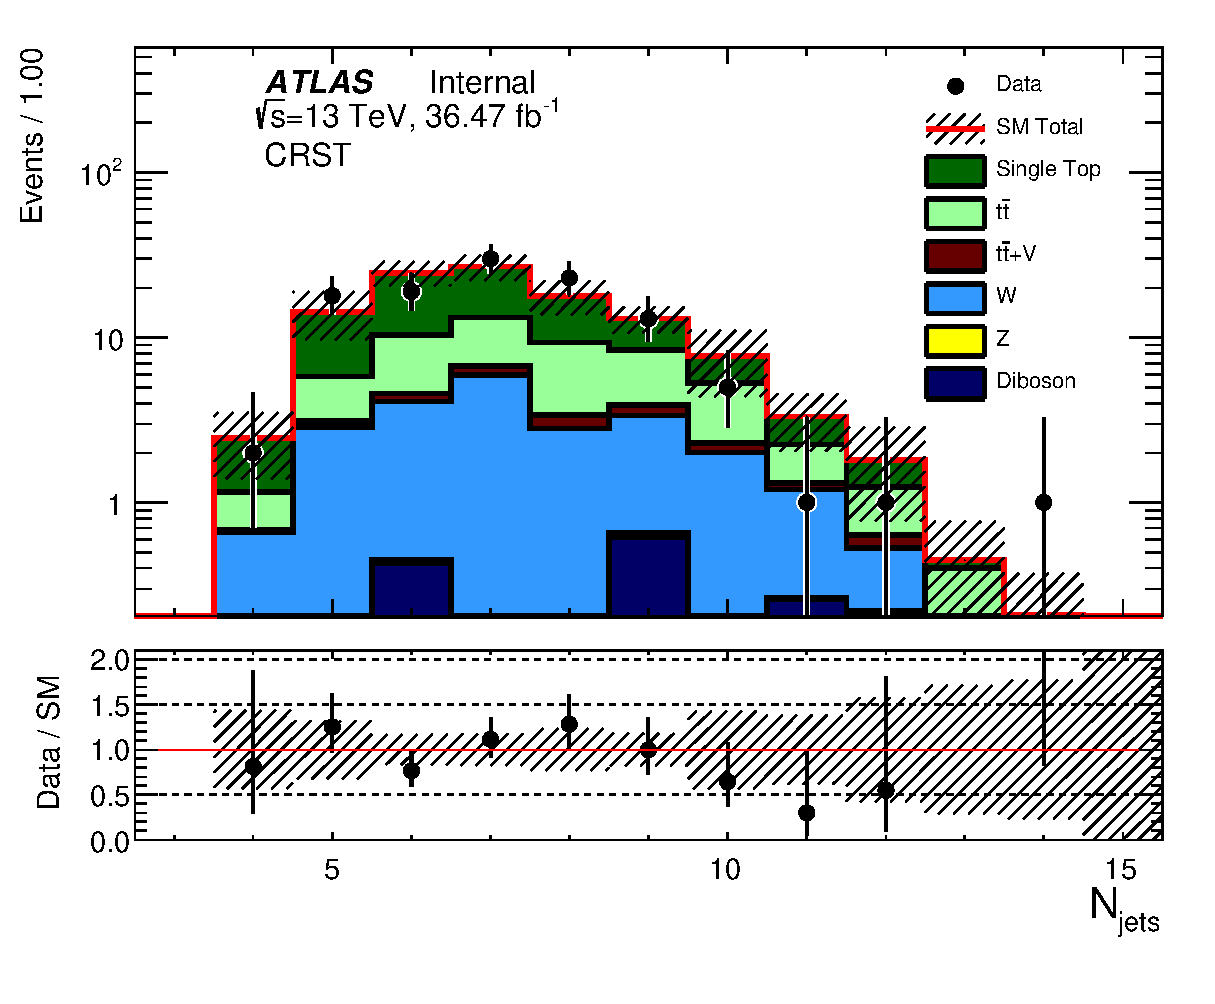
\includegraphics[width=\textwidth]{figures/singleTop/postfit/NJets_CRST_log.eps}
                \caption{ }
    \end{subfigure}
      \begin{subfigure}[b]{0.40\textwidth}    
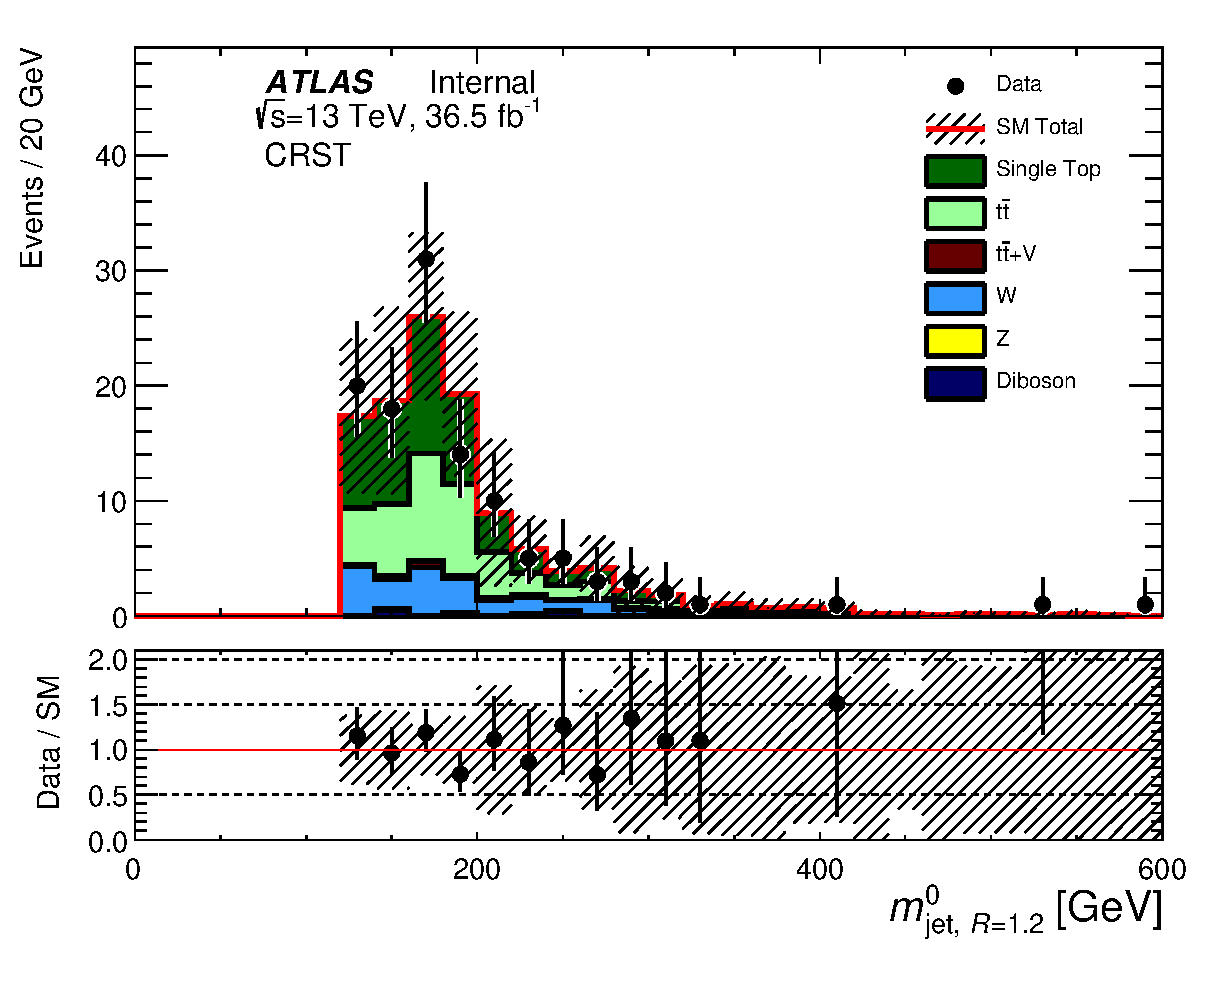
\includegraphics[width=\textwidth]{figures/singleTop/postfit/AntiKt12M_0__CRST.eps}
                \caption{ }
    \end{subfigure}
      \begin{subfigure}[b]{0.40\textwidth}    
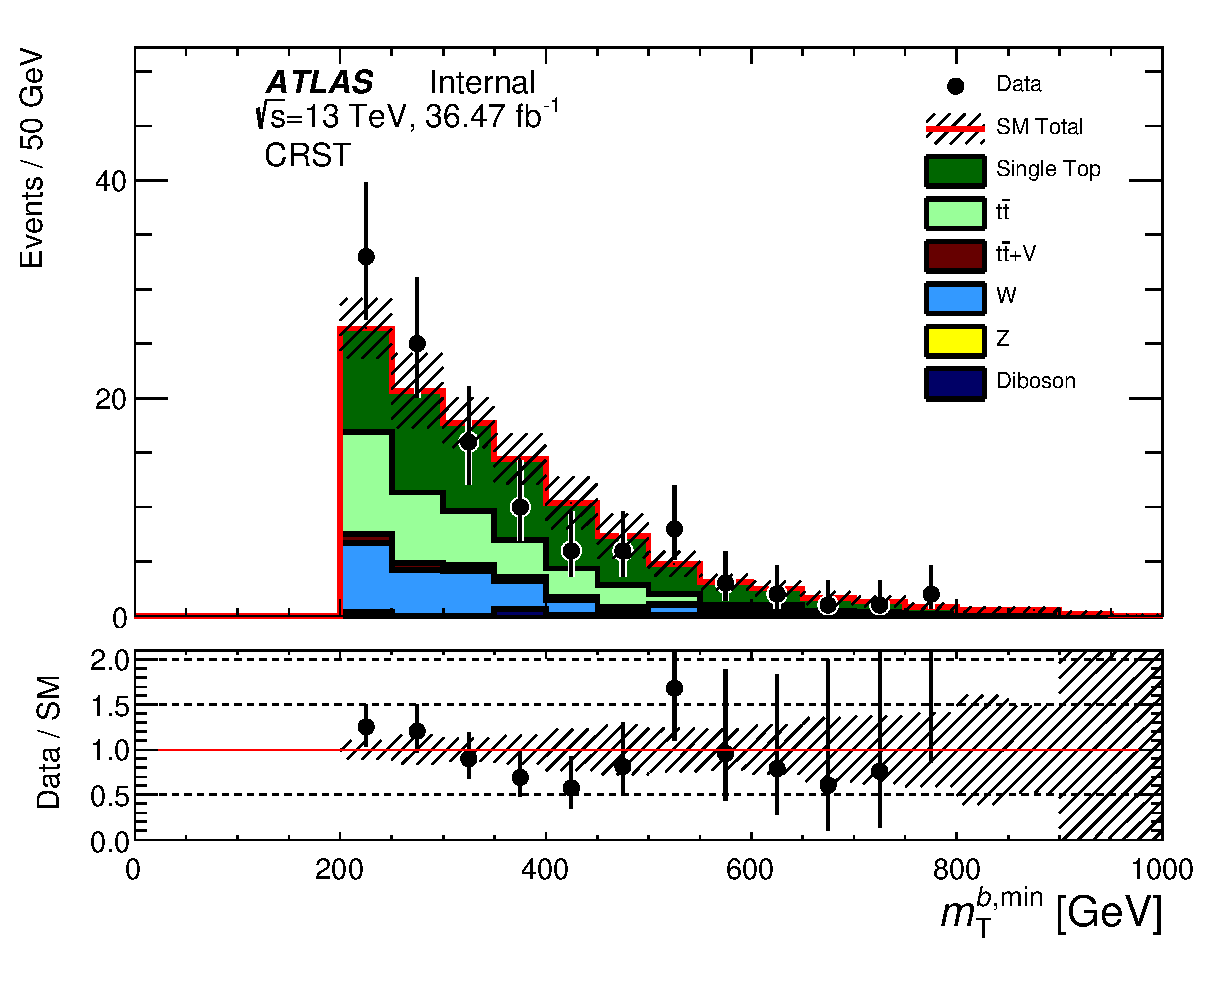
\includegraphics[width=\textwidth]{figures/singleTop/postfit/MtBMin_CRST.eps}
                \caption{ }
    \end{subfigure}
%      \begin{subfigure}[b]{0.40\textwidth}    
%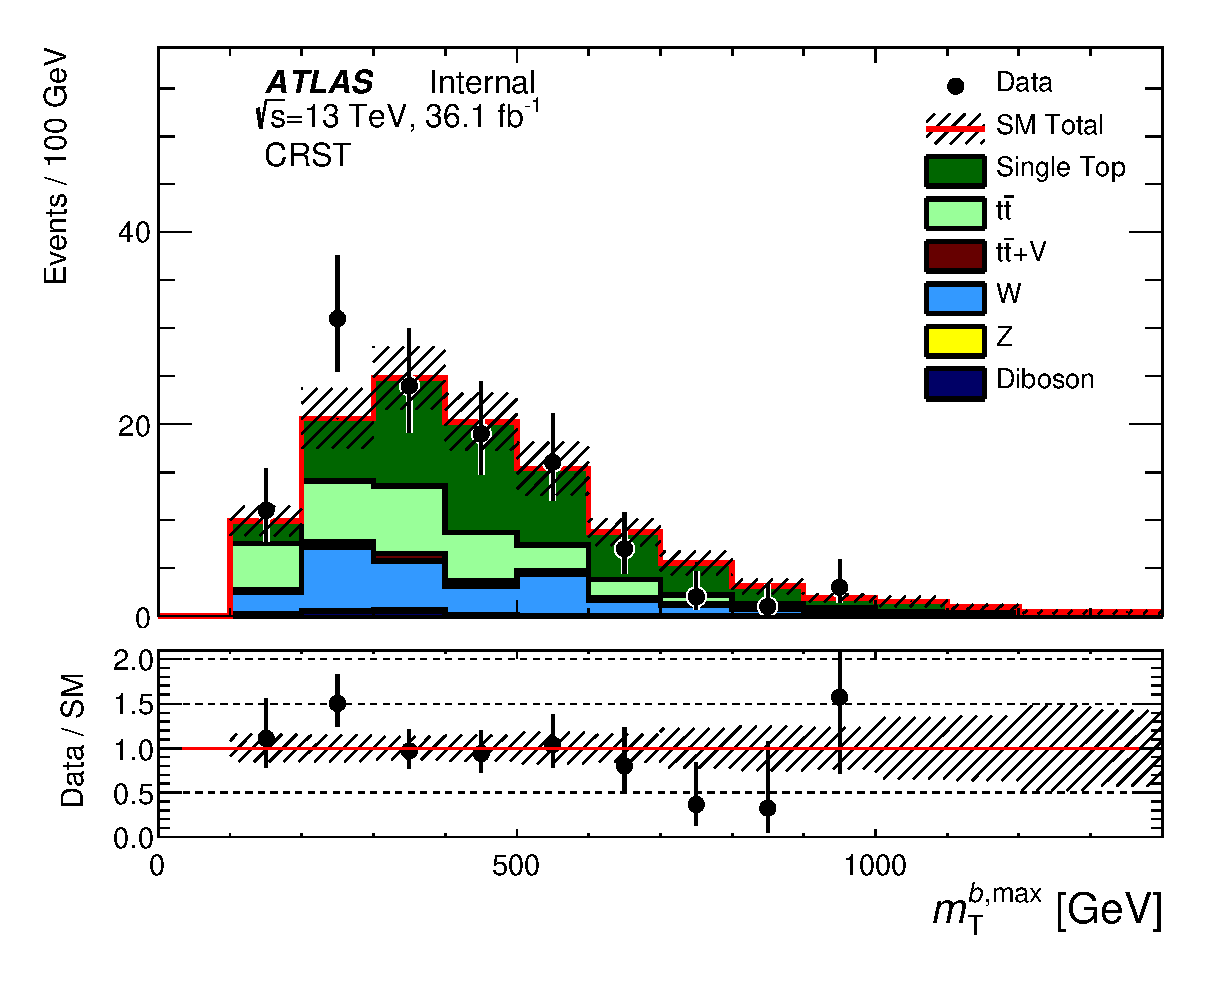
\includegraphics[width=\textwidth]{figures/singleTop/postfit/MtBMax_CRST.eps}
      \begin{subfigure}[b]{0.40\textwidth}    
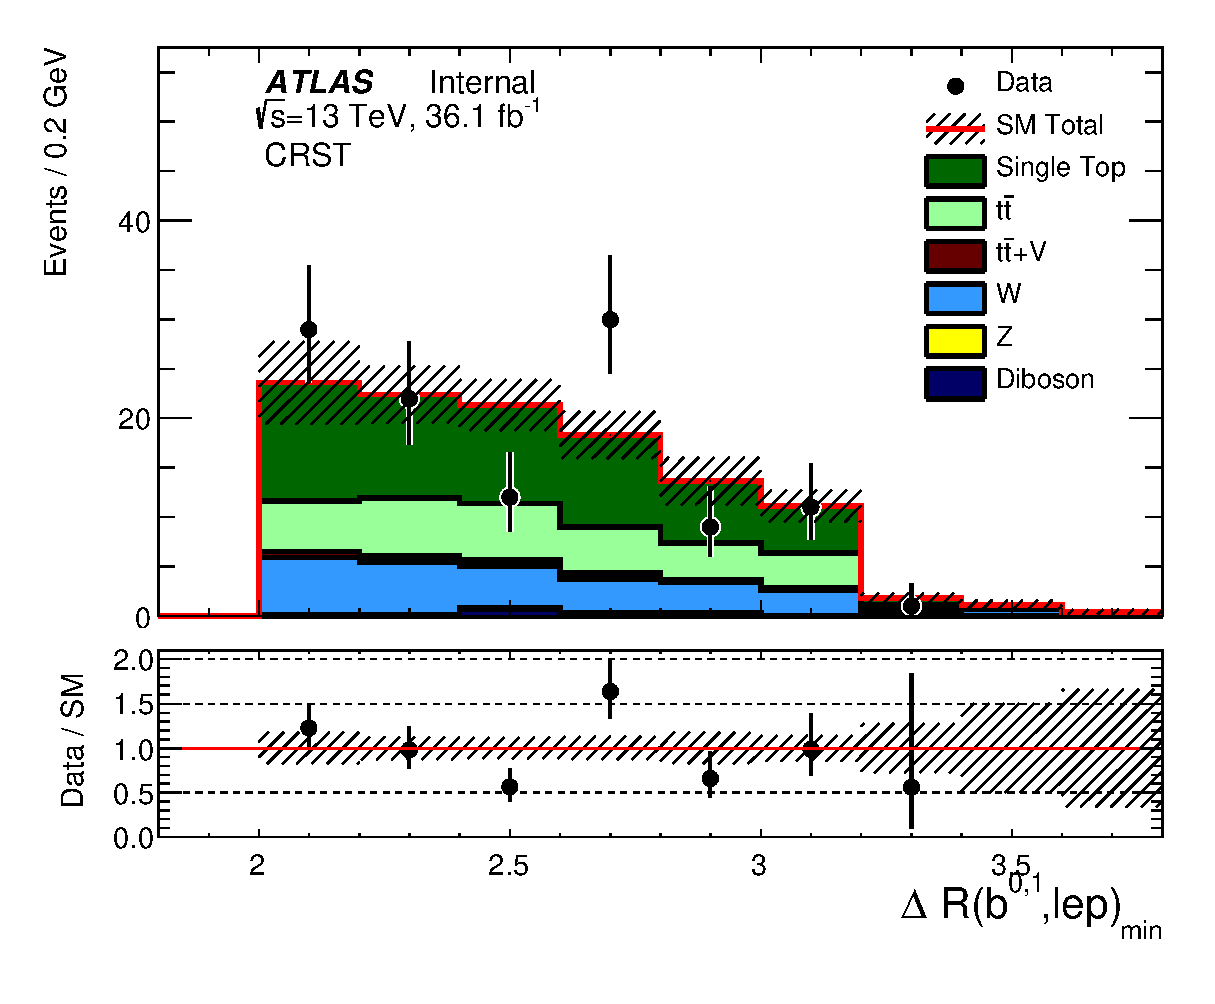
\includegraphics[width=\textwidth]{figures/singleTop/postfit/MinDRBLep_CRST.eps}
                \caption{ }
    \end{subfigure}
      \begin{subfigure}[b]{0.40\textwidth}    
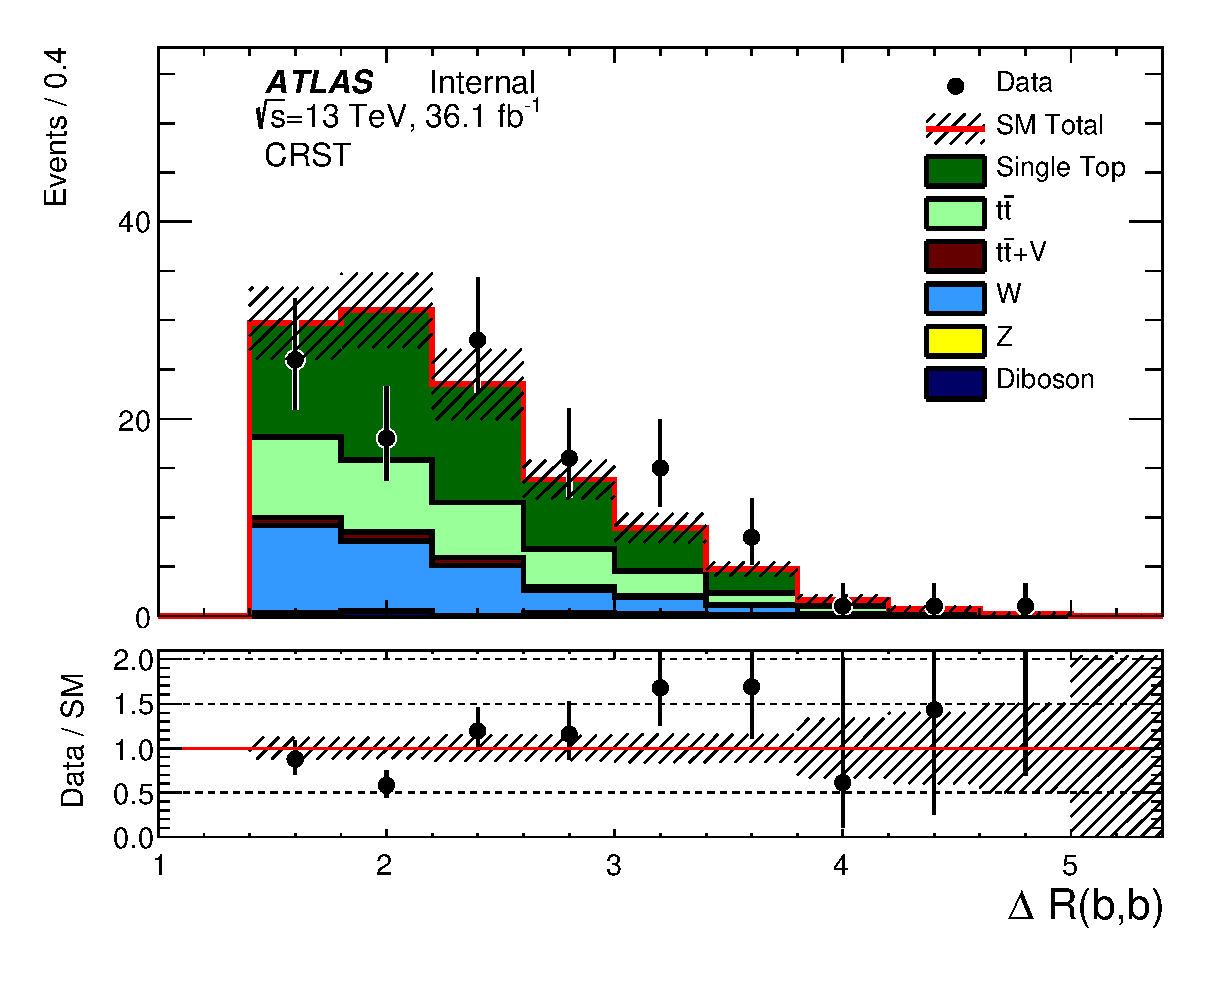
\includegraphics[width=\textwidth]{figures/singleTop/postfit/DRBB_CRST.eps}
                \caption{ }
    \end{subfigure}
%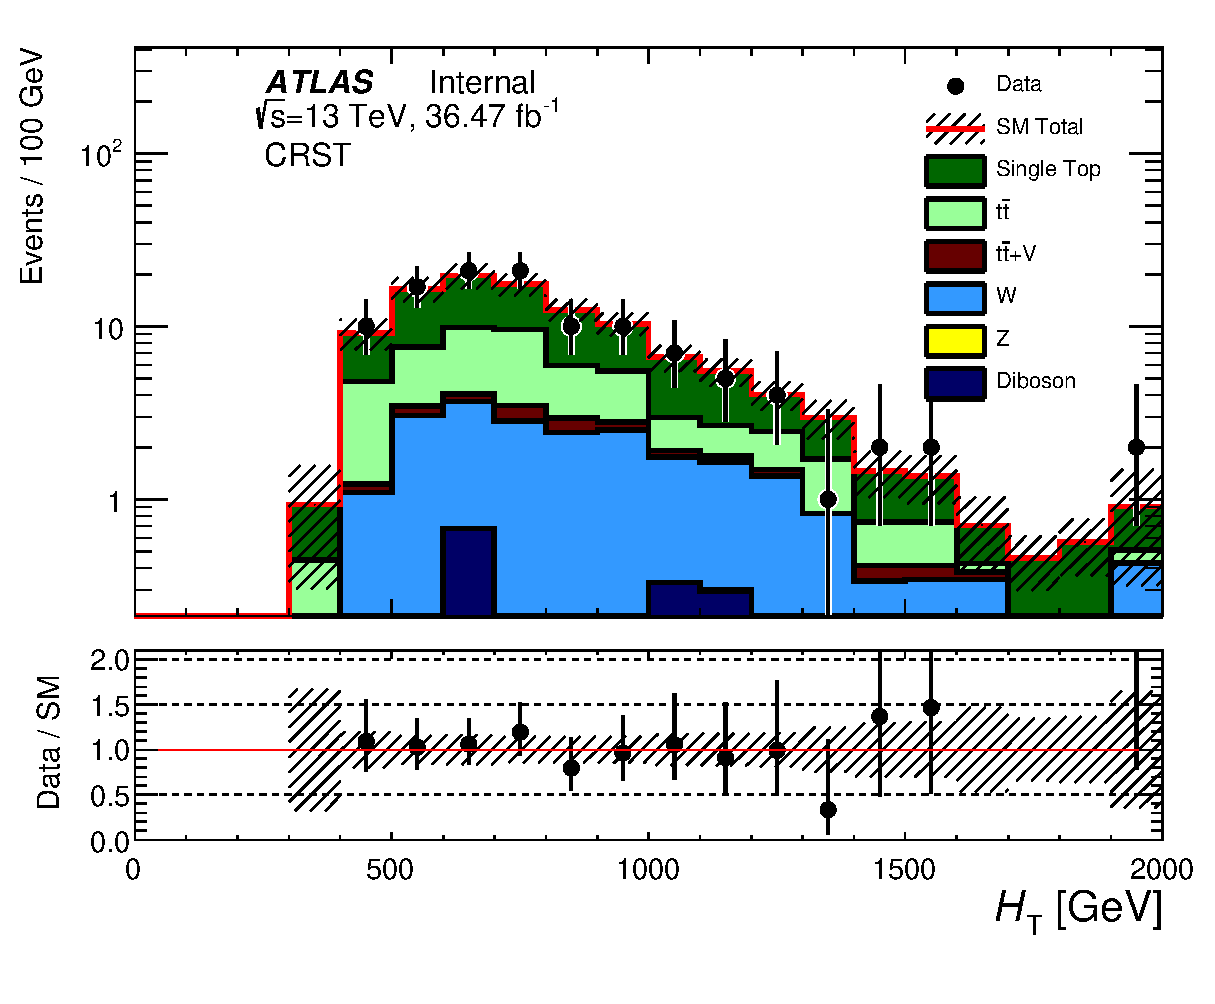
\includegraphics[width=\textwidth]{figures/singleTop/postfit/Ht_CRST_log.eps}
%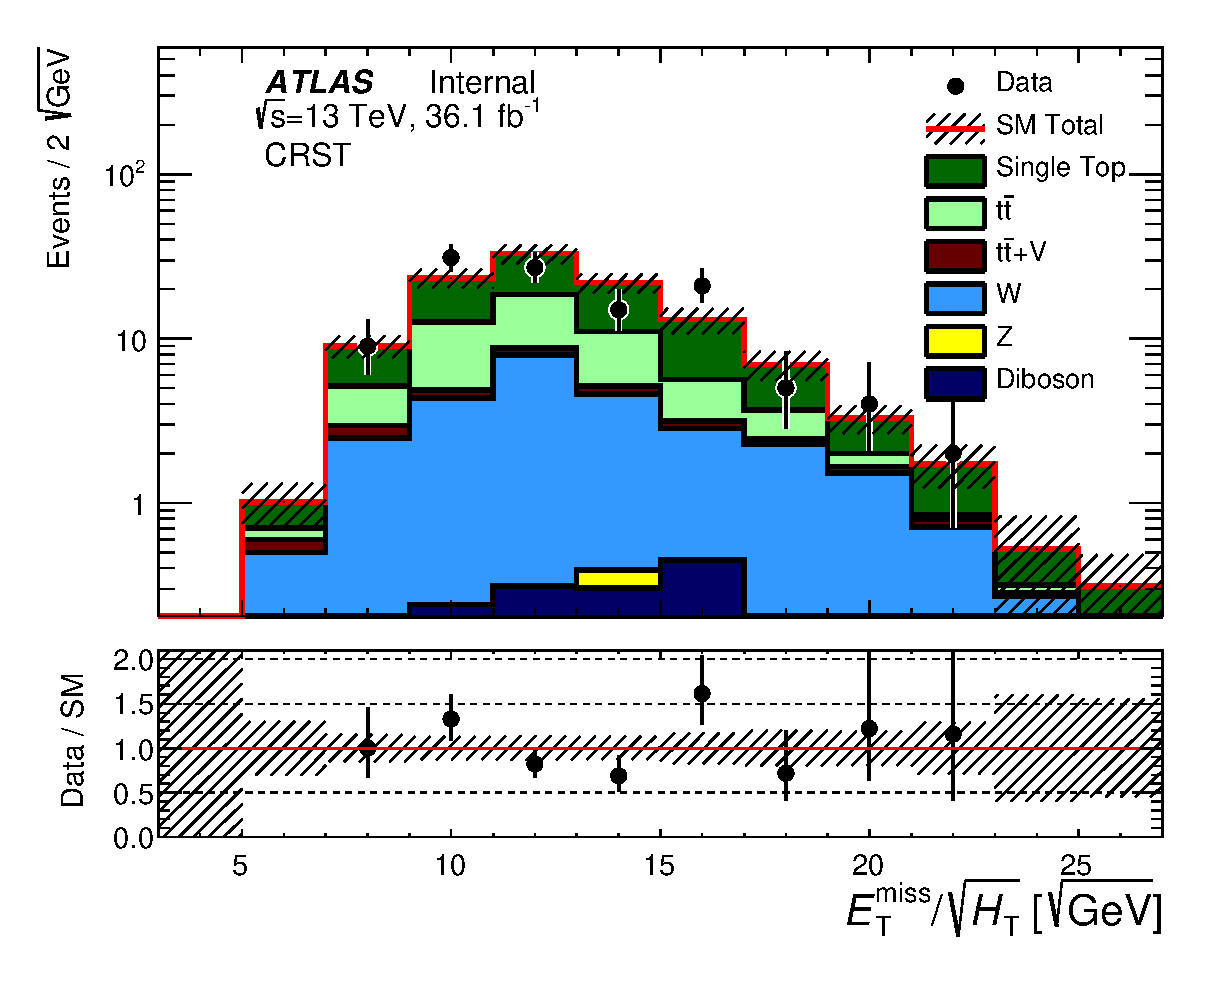
\includegraphics[width=\textwidth]{figures/singleTop/postfit/HtSig_CRST_log.eps}
\end{center}
\caption[Single-top control region distributions for $\intlumi$ $\ifb$ of data after a simultaneous fit to all control regions]{Single-top control region distributions for $\intlumi$ $\ifb$ of data after a simultaneous fit to all control regions. The kinematic variables include (a) $\met$ (b) number of jets (c) $\mantikttwelvezero$ (d) $\mtbmin$ (e) $\mindrblep$ (f) $\drbjetbjet$. The ratio between data and MC is shown in the bottom panel. The hashed area on the expected SM background represents the uncertainty due to experimental systematics and MC statistics.}
\label{fig:CRST}
\end{figure}

\pagebreak

\begin{figure}[h!]
  \begin{center}
      \begin{subfigure}[b]{0.40\textwidth}    
    	 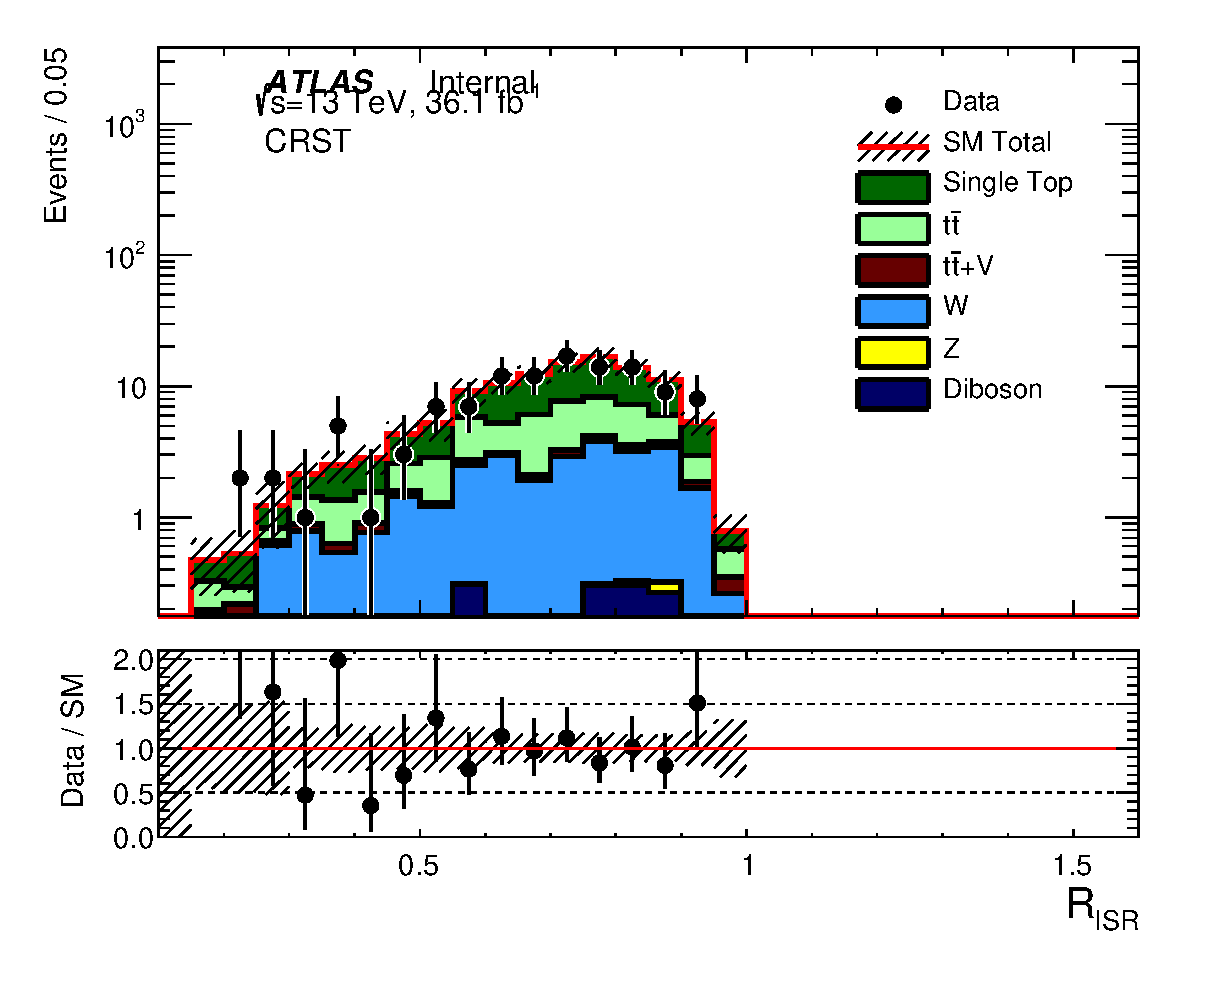
\includegraphics[width=\textwidth]{figures/plotRegion/CA_RISR_CRST_log.eps}
                \caption{ }
    \end{subfigure}
        \begin{subfigure}[b]{0.40\textwidth}    
    	 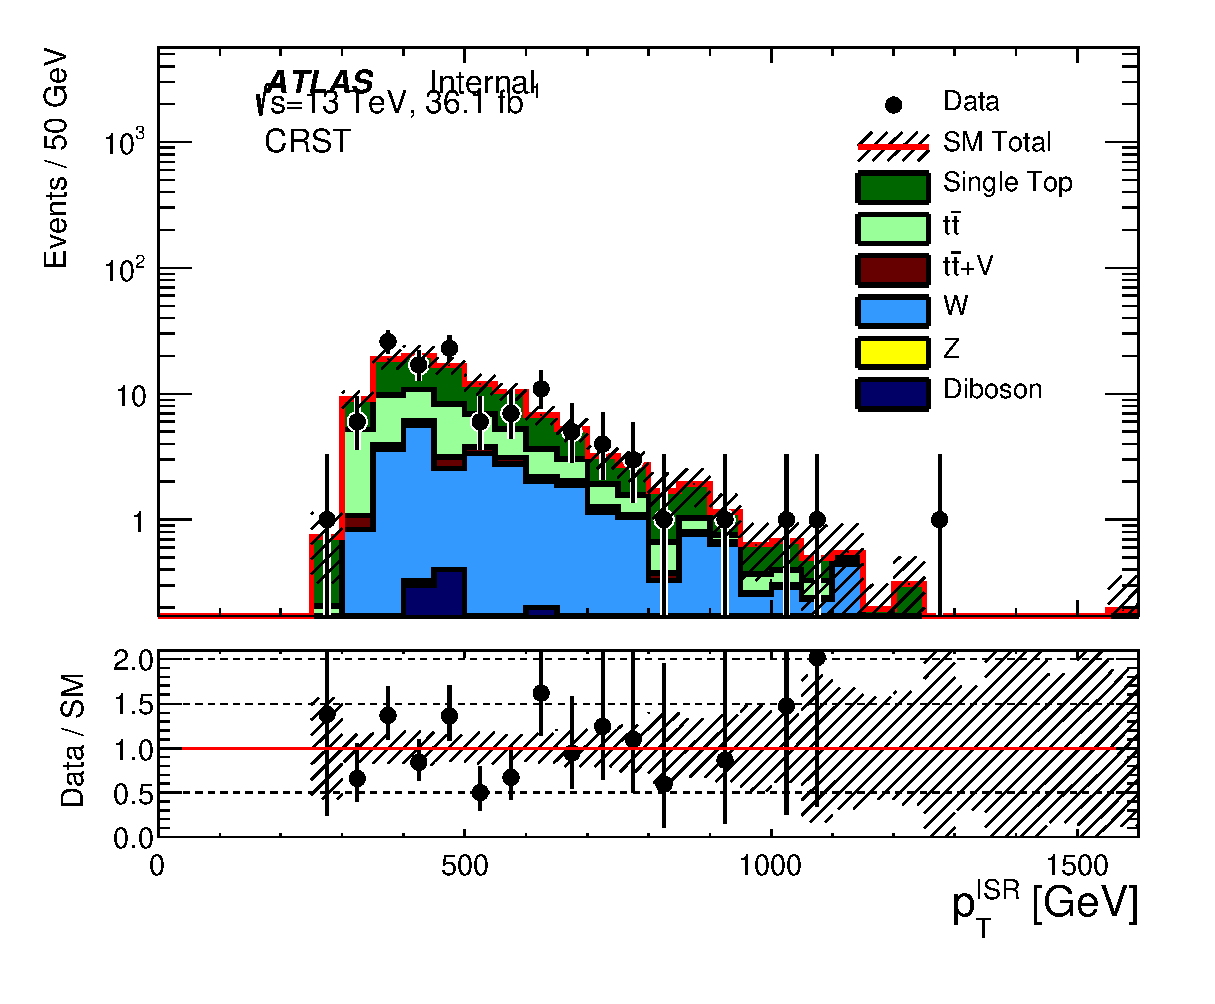
\includegraphics[width=\textwidth]{figures/plotRegion/CA_PTISR_CRST_log.eps}
                \caption{ }
    \end{subfigure}
    \begin{subfigure}[b]{0.40\textwidth}    
    	 \includegraphics[width=\textwidth]{figures/plotRegion/CA_dphiISRI_CRST_log.eps}
                \caption{ }
    \end{subfigure}
    \begin{subfigure}[b]{0.40\textwidth}    
    	 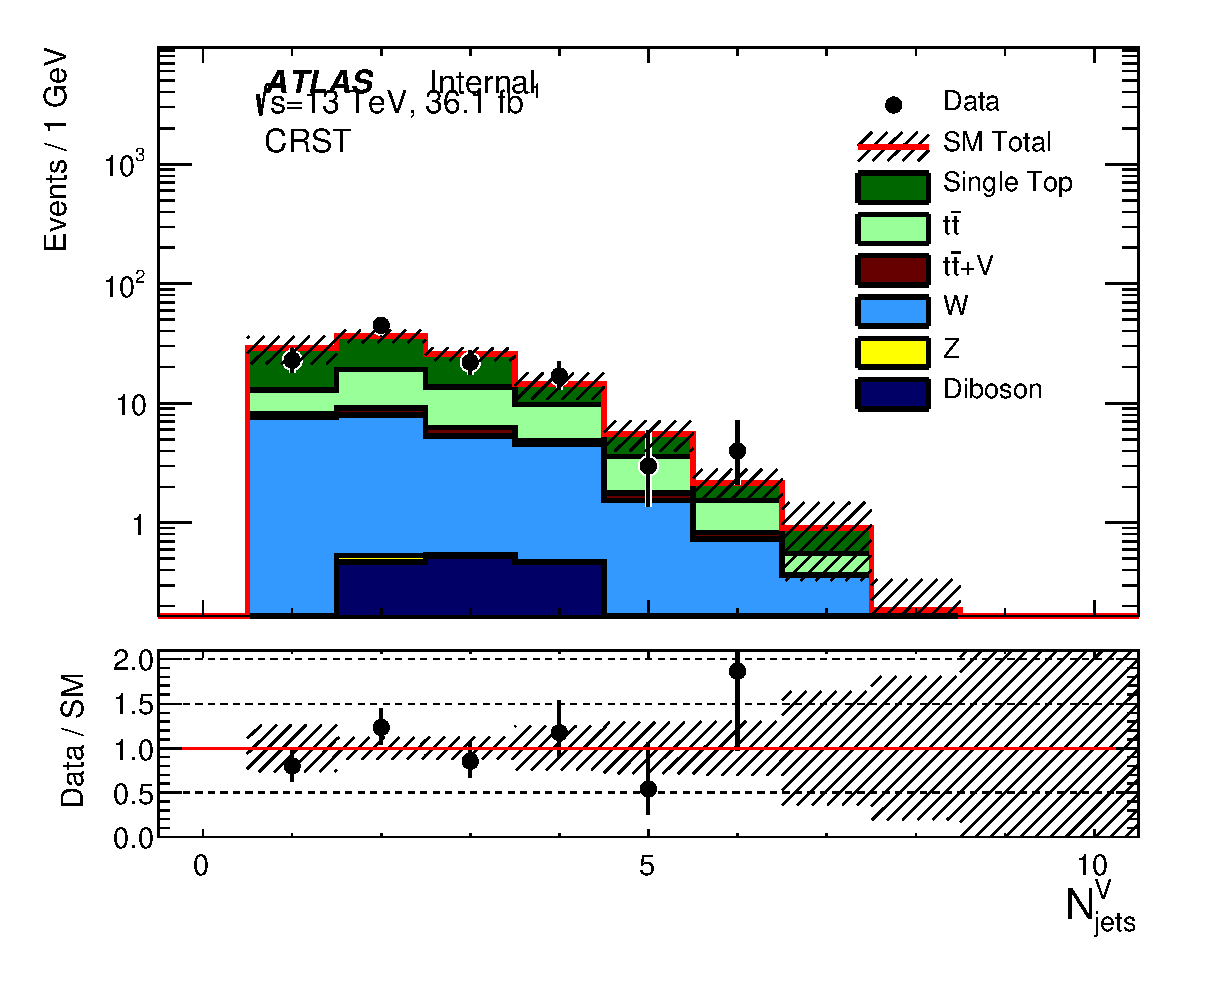
\includegraphics[width=\textwidth]{figures/plotRegion/CA_NjV_CRST_log.eps}
                \caption{ }
    \end{subfigure}
    \begin{subfigure}[b]{0.40\textwidth}    
    	 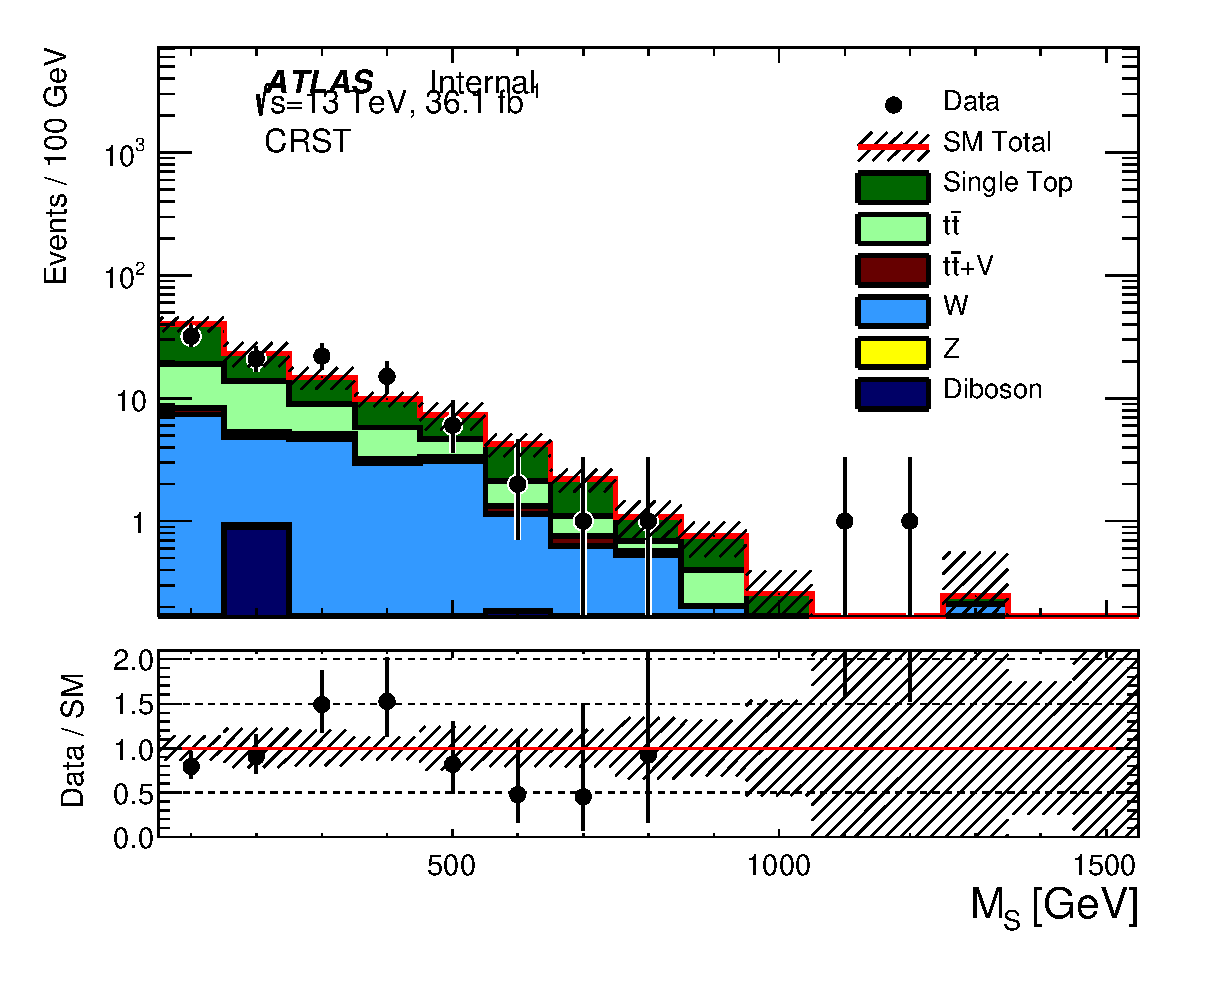
\includegraphics[width=\textwidth]{figures/plotRegion/CA_MS_CRST_log.eps}
                \caption{ }
    \end{subfigure}
    \begin{subfigure}[b]{0.40\textwidth}    
    	 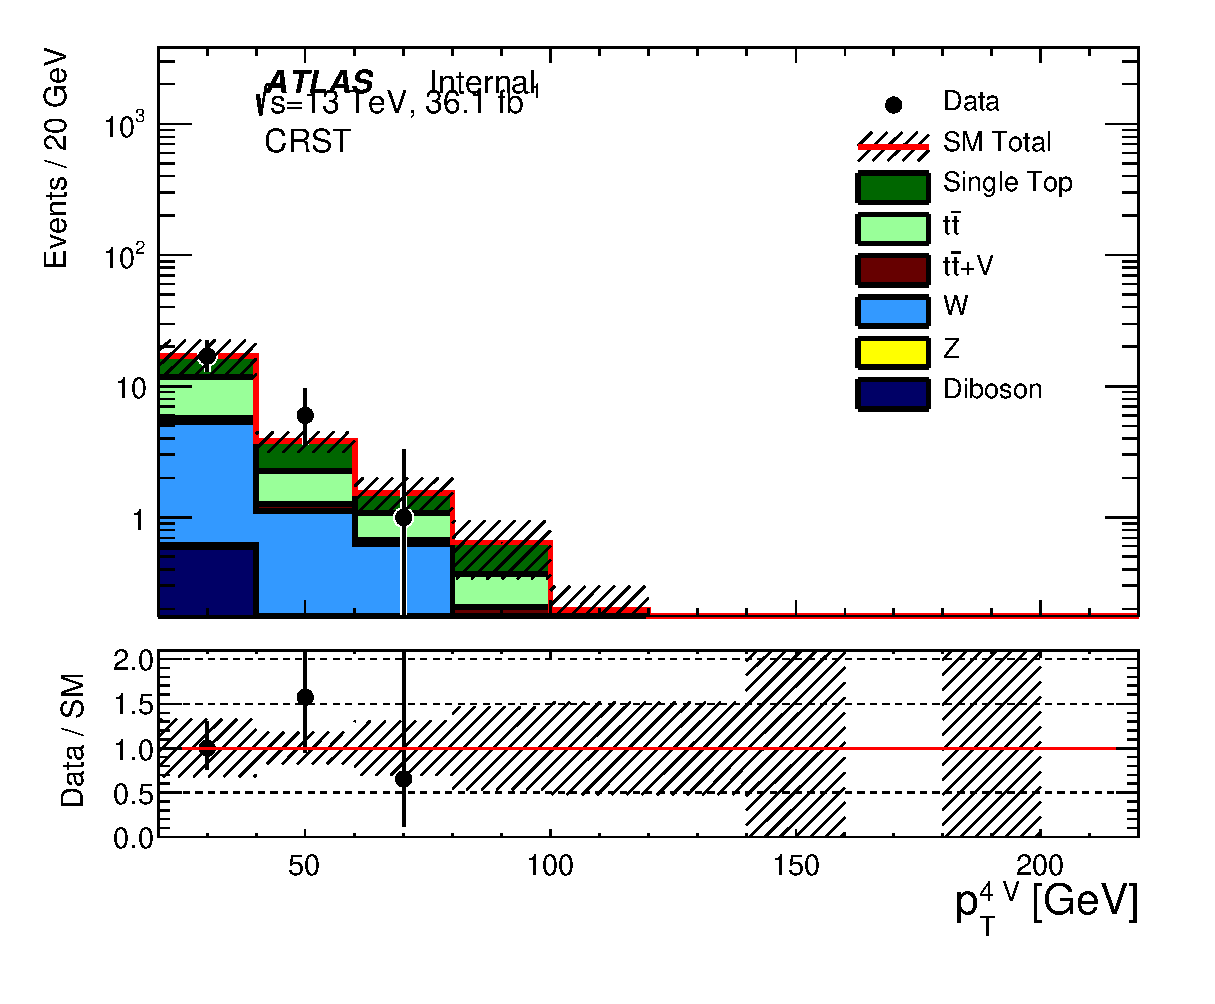
\includegraphics[width=\textwidth]{figures/plotRegion/CA_pTjV4_CRST_log.eps}
               \caption{ }
    \end{subfigure}
     \caption[Single-top control region distributions for \intlumi\ \ifb\ of data after a simultaneous fit to all control regions.]{ Single-top control region distributions for \intlumi\ \ifb\ of data after a simultaneous fit to all control regions. The kinematic variables include (a) $\RISR$ (b) $\PTISR$ (c) $\dphiISRI$ (d) $\NjV$ (e) $\MS$ (f) $\pTjV$.  The ratio between data and MC is shown in the bottom panel. The hashed area on the expected SM background represents the uncertainty due to experimental systematics and MC statistics.
     }
  \label{fig:CRST1}
    \end{center}
\end{figure}

\pagebreak



\begin{table}[h!]
\begin{center}
\setlength{\tabcolsep}{0.0pc}
{\small
%%
\begin{tabular*}{\textwidth}{@{\extracolsep{\fill}}lr}
\noalign{\smallskip}\hline\noalign{\smallskip}
{\bf CRother yields}             & CRST              \\[-0.05cm]
\noalign{\smallskip}\hline\noalign{\smallskip}
%%
Observed events                & $114$                    \\
\noalign{\smallskip}\hline\noalign{\smallskip}
%%
Fitted bkg events                & $113.93 \pm 10.65$              \\
\noalign{\smallskip}\hline\noalign{\smallskip}
%%
        Fitted TTbar events              & $29.80 \pm 10.52$              \\
%%
        Fitted Wjets events           & $26.36 \pm 5.82$              \\
%%
        Fitted Zjets events              & $0.10 \pm 0.07$              \\
%%
        Fitted TtbarV events             & $3.14 \pm 0.73$              \\
%%
        Fitted SingleTop events            & $52.95 \pm 17.45$              \\
%%
        Fitted Diboson events                & $1.59 \pm 0.79$              \\
%%
        Fitted Multijets events                & $0.00 \pm 0.00$              \\
%%     
 \noalign{\smallskip}\hline\noalign{\smallskip}
%%
MC exp. SM events                    & $102.60 \pm 12.42$              \\
\noalign{\smallskip}\hline\noalign{\smallskip}
%%
        MC exp. TTbar events             & $32.24 \pm 11.17$              \\
%%
        MC exp. Wjets events             & $20.83 \pm 3.02$              \\
%%
        MC exp. Zjets events                & $0.09 \pm 0.06$              \\
%%
        MC exp. TtbarV events              & $2.44 \pm 0.42$              \\
%%
        MC exp. SingleTop events            & $45.42 \pm 1.32$              \\
%%
        MC exp. Diboson events                & $1.58 \pm 0.79$              \\
%%
        MC exp. Multijets events             & $0.00 \pm 0.00$              \\
%%     \\
\noalign{\smallskip}\hline\noalign{\smallskip}
Fitted single top normalization scale factor & $0.707 \pm 0.050$ \\
\noalign{\smallskip}\hline\noalign{\smallskip}
\end{tabular*}
%%%
}
\end{center}
\caption[Single top control region MC Yield and background-only fit results for $\intlumi$ $\ifb$ of data]{Single top control region MC Yield and background-only fit results for $\intlumi$ $\ifb$ of data. MC exp. events are expected background rates directly from MC predictions.  Fitted background event rates are the expected background rates after normalizing the MC to data by simultaneously fitting all control regions using a background only fit.  The fitted $W$+jets normalization scale factor is equal to (Fitted single top events)/(MC exp. single top events). The quoted uncertainties include statistical and systematic uncertainties. }
\label{table.bkgonly.CRST}
\end{table}
%


\subsection{Standard Model \ttbar+Z}
\label{sec:Bkg:ttV}

\indent $\ttbar$ produced in conjunction with a $Z$ boson consists of about 1\% of the background in the signal region.  We estimate the amount of $\ttbar+\Zboson$ using a $\ttbar+\gamma$ control region. \\

\indent Using the charged leptonic $Z$ boson decays to design a control region to estimate the $\ttbar+Z$ background would produce a control region with small systematic uncertainty. However, such a control region tends to have low statistics because $Z \rightarrow ee/\mu\mu$ has a lower branching fraction than $Z \rightarrow \nu\nu$.  A dilepton control region also contains a large contribution from SM $\ttbar$ and $Z$ + jets. \\

\indent We take another data driven approach by building a one-lepton control region for $\ttbar+\gamma$.  $\ttbar+\gamma$ mimics $\ttbar+Z$ as the photon is in many ways like a lighter $Z$ boson.  The control region is designed to minimize theoretical uncertainties due to the extrapolation from the $\gamma$ in the control region to the $\Zboson$ in the signal region. \\

\indent We require exactly one {\tt Signal} photon and one {\tt Signal} lepton.  The lepton is not treated as a jet for the purpose of jet multiplicity and jet $\pt$ requirements unlike in the other one lepton control regions.  We also trigger on leptons instead of $\met$ in this region. The lepton triggers used are defined in Table \ref{tb:lepTriggers}.  \\

\begin{table}[h!]
  \begin{center}
    \begin{tabular}{c|c} \hline\hline
      Channel & Trigger \\  \hline
              & {\bf Data 2015} \\ \hline
      Electron & \verb+HLT_e24_lhmedium_L1EM20VH+  \\
      	            & \verb+HLT_e60_lhmedium+ \\
	            & \verb+HLT_e120_lhloose+         \\  
      Muon & \verb+HLT_mu20_iloose_L1MU15+ \\
      	       & \verb+HLT_mu50+ \\
      \hline
              & {\bf Data 2016} \\ \hline
      Electron & \verb+HLT_e26_lhtight_nod0_ivarloose+ \\
                     &\verb+HLT_e60_lhmedium_nod0+ \\
                     &\verb+HLT_e140_lhloose_nod0+         \\ 
      Muon & \verb+HLT_mu26_ivarmedium+ \\ 
                & \verb+HLT_mu50+ \\
      \hline \hline
    \end{tabular}
  \end{center}
  \caption{Single Lepton triggers used in the $\ttbar+\gamma$ control region.  The electron triggers correspond to the a $\pt$ threshold of 24, 26, 60, 120, and 140 $\gev$ respectively.  The muon triggers correspond to $\pt$ thresholds of 20,26 and 50 $\gev$. }
  \label{tb:lepTriggers}
\end{table}

\indent We require the photon $\pt$ be greater than $150\gev$.  The high $\pt$ photon ensures that we are in a region of phase space where the $\gamma$ $\pt$ shape will mimic the heavier $\Zboson$ $\pt$ distribution.  The true $\gamma$ $\pt$ and the $\Zboson$ $\pt$ distributions are shown in Figure \ref{fig:ttZ_vs_ttGamma_pt} after selecting for a boson $\pt$ with greater than $150 \gev$.  We add a systematic uncertainty to account for the difference between the $\gamma$ and $\Zboson$ $\pt$ spectrum. \\

\pagebreak

\begin{figure}[h!]
\centering
\includegraphics[scale=0.4, angle=270]{figures/ttGamma/TruthStudies/Pt150.pdf}
\caption[$\gamma$ and $\Zboson$ $\pT$ distributions in MC simulation with no detector resolution effects]{$\gamma$ and $\Zboson$ $\pT$ distributions in MC simulation with no detector resolution effects.  A selection of $\pt > 150 \gev$ has been applied.}
\label{fig:ttZ_vs_ttGamma_pt}
\end{figure}

\indent The $\ttbar+\gamma$ control region is defined in Table~\ref{tb:ttG_1lepSel}.  The expected background and data yields in the $\ttbar+\gamma$ control region is given in Table \ref{table.bkgonly.CRTTgamma}. \\

\begin{table}[h!]
  \begin{center}
    \begin{tabular}{c|c}
      \hline \hline
      Selection                 & Requirement     \\
      \hline \hline
      Event selection & Event cleaning \\
      \hline
       Trigger  & 1L Triggers  \\  \hline
      Leptons & $= 1$ \\
      Lepton \pt & 28 $\GeV$ \\
      \hline
      Photons & exactly 1\\
      \hline
      jet multiplicity & $ \ge 4 $ \\
      \hline
      Jet \pT\ & (80,80,40,40) GeV \\
      \hline
      b-jet multiplicity & $\ge 2$ \\
      \hline
      $\gamma$ \pT\ & $> 150$ GeV \\
      \hline\hline
    \end{tabular}
  \end{center}
    \caption[Selections for the $\ttbar+\gamma$ one lepton control region]{Selections for the $\ttbar+\gamma$ one lepton control region. The one lepton triggers as described in Table~\ref{tb:lepTriggers}}
      \label{tb:ttG_1lepSel}
\end{table}




\begin{table}[!h]
\begin{center}
\setlength{\tabcolsep}{0.0pc}
{\small
%%
\begin{tabular*}{\textwidth}{@{\extracolsep{\fill}}lr}
\noalign{\smallskip}\hline\noalign{\smallskip}
{\bf CRTTgamma yields}           & CRTTGamma              \\[-0.05cm]
\noalign{\smallskip}\hline\noalign{\smallskip}
%%
Observed events          & $161$                    \\
\noalign{\smallskip}\hline\noalign{\smallskip}
%%
Fitted bkg events         & $161.19 \pm 14.03$              \\
\noalign{\smallskip}\hline\noalign{\smallskip}
%%
        Fitted TTbar events         & $4.75_{-4.75}^{+9.52}$              \\
%%
        Fitted Wjets events         & $0.05 \pm 0.01$              \\
%%
        Fitted Zjets events         & $0.75 \pm 0.19$              \\
%%
        Fitted TtbarV events         & $3.01 \pm 0.42$              \\
%%
        Fitted TtbarGamma events         & $143.96 \pm 13.37$              \\
%%
        Fitted SingleTop events         & $2.40 \pm 0.84$              \\
%%
        Fitted Diboson events         & $0.00 \pm 0.00$              \\
%%
        Fitted VGamma events         & $6.27 \pm 1.63$              \\
%%     
 \noalign{\smallskip}\hline\noalign{\smallskip}
%%
MC exp. SM events              & $128.31 \pm 18.89$              \\
\noalign{\smallskip}\hline\noalign{\smallskip}
%%
        MC exp. TTbar events         & $5.14_{-5.14}^{+11.21}$              \\
%%
        MC exp. Wjets events         & $0.04 \pm 0.01$              \\
%%
        MC exp. Zjets events         & $0.66 \pm 0.13$              \\
%%
        MC exp. TtbarV events         & $2.34 \pm 0.37$              \\
%%
        MC exp. TtbarGamma events         & $111.77 \pm 13.41$              \\
%%
        MC exp. SingleTop events         & $2.07 \pm 0.40$              \\
%%
        MC exp. Diboson events         & $0.00 \pm 0.00$              \\
%%
        MC exp. VGamma events         & $6.29 \pm 1.64$              \\
%%     \\
\noalign{\smallskip}\hline\noalign{\smallskip}
Fitted $\ttbar+\gamma$ normalization scale factor & $1.29 \pm 0.20$ \\
\noalign{\smallskip}\hline\noalign{\smallskip}
\end{tabular*}
%%%
}
\end{center}
\caption[$\ttbar+\gamma$ control region MC Yield and background-only fit results for $\intlumi$ $\ifb$ of data]{$\ttbar+\gamma$ control region MC Yield and background-only fit results for $\intlumi$ $\ifb$ of data. MC exp. events are expected background rates directly from MC predictions.  Fitted background event rates are the expected background rates after normalizing the MC to data by simultaneously fitting all control regions using a background-only fit.  The fitted $\ttbar+\gamma$ normalization scale factor is equal to (Fitted $\ttbar+\gamma$ events)/(MC exp. $\ttbar+\gamma$ events). The quoted uncertainties include statistical and systematic uncertainties. }
\label{table.bkgonly.CRTTgamma}
\end{table}
%

\indent Kinematic distributions in the $\ttbar+\gamma$ control region are shown in Figure ~\ref{fig:ttgamma}  The MC background has been normalized to data by performing a simultaneous fit to all the control regions.  The hashed bands on the total SM background correspond to the total experimental systematical uncertainty plus the MC statistical uncertainty.   \\

\pagebreak

\begin{figure}[h!]
\begin{center}
      \begin{subfigure}[b]{0.40\textwidth}    
\includegraphics[width=\textwidth]{figures/ttGamma/Met_CRTTGamma_withRatio_log.eps}
                 \caption{ }
    \end{subfigure}
      \begin{subfigure}[b]{0.40\textwidth}    
      \includegraphics[width=\textwidth]{figures/ttGamma/postfit/NJets_CRTTGamma_log.eps}
                 \caption{ }
    \end{subfigure}
      \begin{subfigure}[b]{0.40\textwidth}    
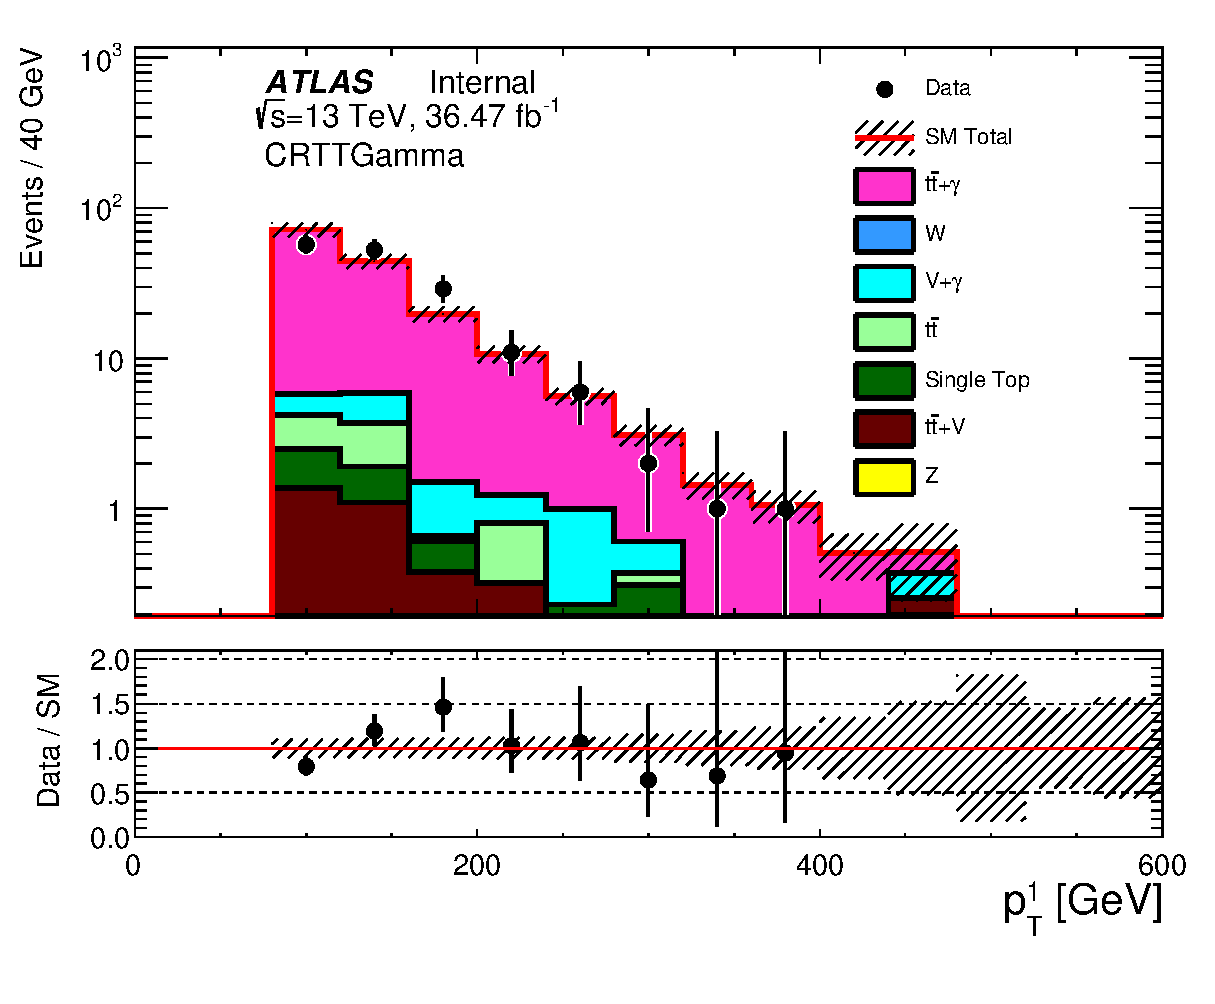
\includegraphics[width=\textwidth]{figures/ttGamma/postfit/JetPt_1__CRTTGamma_log.eps}
                 \caption{ }
    \end{subfigure}
      \begin{subfigure}[b]{0.40\textwidth}    
\includegraphics[width=\textwidth]{figures/ttGamma/postfit/JetPt_4__CRTTGamma_log.eps}
                 \caption{ }
    \end{subfigure}
%      \begin{subfigure}[b]{0.40\textwidth}    
%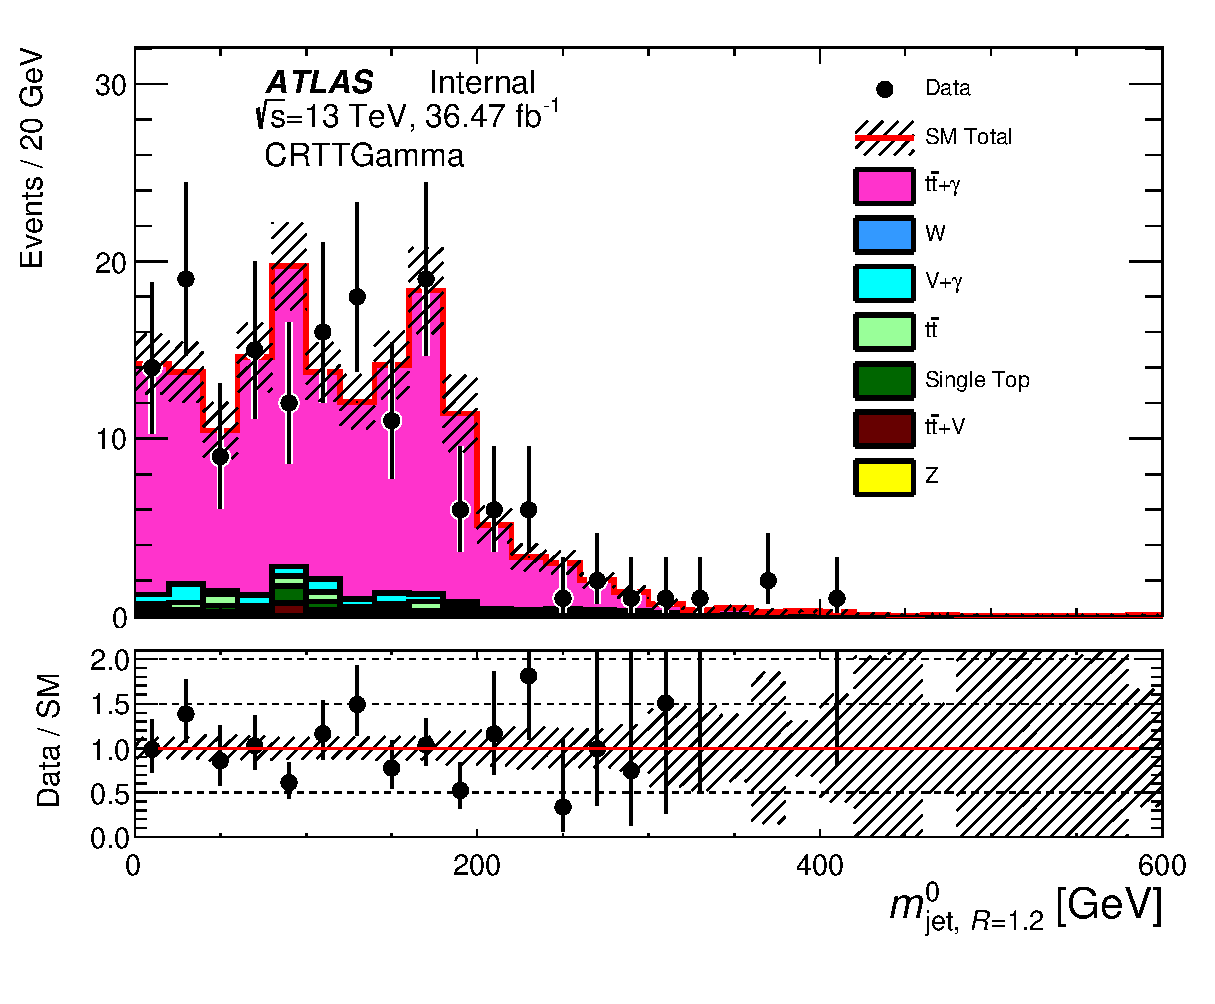
\includegraphics[width=\textwidth]{figures/ttGamma/postfit/AntiKt12M_0__CRTTGamma.eps}
%                 \caption{ }
%    \end{subfigure}
%      \begin{subfigure}[b]{0.40\textwidth}    
%\includegraphics[width=\textwidth]{figures/ttGamma/MtMetLep_CRTTGamma_withRatio_log.eps}
%                 \caption{ }
%    \end{subfigure}
\caption[Distributions of select kinematic variables in the $\ttbar+\gamma$ control region]{ Distributions of select kinematic variables in the $\ttbar+\gamma$ control region. Kinematic variables shown include (a) $\met$ (b) number of jets (c) $\pt$ of the 2nd highest $\pt$ jet (d) $\pt$ of the 5th highest $\pt$ jet. The hashed area in both the top and lower panel represents the uncertainty due to MC statistics.}
\label{fig:ttgamma}
\end{center}
\end{figure}







\subsection{Standard Model Z+Jets}
\label{sec:Bkg:zjet}

Z+jets consist of 3 percent of all backgrounds in the SR.  The percentage of Z+jets is higher in high $\RISR$ bins.  The percentage Z+jets rises to 7 percent in $\RISR$ between 0.6 and 0.8.  We use just the MC prediction for Z+jets because the rate of Z+jet is so low.  We assign an 100 percent theory uncertainty to the Z+jets rate in the SR.  \\
The ttbar validation region described in section \ref{sec:Bkg:ttbar:VR} has a larger fraction of Z+jets event then those in the SR.  The ttbar VR is kinematically similar to those of the SR with some loser cuts on jet multiplicity and ISR, \MET correlations.  The good agreement between data and MC in the ttbar VR is evidence that the Z+jets MC cannot be wrong by more than 100 percent.  \\
\subsection{Standard Model Diboson}
\label{sec:Bkg:diboson}

\indent Standard Model dibosons consist of approximately 1\% of the background in the signal region.  The background is negligible and we only use MC predictions for background estimation. We apply a 50\% theory uncertainty on the diboson background. \\
\subsection{Standard Model QCD Multijet and all Hadronic $\ttbar$}
\label{sec:Bkg:QCD}

\indent Both QCD multijet and all hadronic $\ttbar$ creates little intrinsic $\met$. Instead misreconstructed jets can cause an imbalance in the total event $E_t$ and generate fake $\met$.  QCD contributions are only significant in the SR bins with low $\RISR < 0.4$ and are estimated using the data driven jet smearing method.  \\

\subsubsection*{The Jet Smearing Method}

\indent The jet smearing method first selects seed events from data with well reconstructed jets and little $\met$.  Seed events are selected according to the criteria listed in table \ref{tab:qcd:seed}. We then repeatedly smear the seed events' jets with a predetermined jet energy response.  The resulting {\tt pesudo-data} events can have potentially large $\met$ due to the smeared jets.  A schematic demonstrating the jet smearing method is shown in figure \ref{fig:jetsmearing}.\\

\begin{figure}[htbp]
\begin{center}
\includegraphics[width=0.45\textwidth]{figures/QCDJetSmearing/jet_smearing.pdf}
\end{center}
\caption{Schematic of the jet smearing method.  A seed event with good jet energy measurements are repeatedly smeared with predetermined jet energy resolutions.  The new $\met$ is calculated as the difference between the seed event's and smeared event's jet momenta plus the original seed event's $\met$.  (Figure taken from \cite{JetSmearing})}
\label{fig:jetsmearing}
\end{figure}

\indent The jet smearing methods have a number of inherent assumptions about the generation of $\met$ in QCD multijet and all hadronic $\ttbar$ background.  These assumptions include: \\

\begin{itemize}
\item The jet response captures all sources of jet $\pt$ measurement fluctuations
\item The $\met$ in multijet events result predominately from mis-measured jets
\item Jet response are independent on the presence of other jet and jet smearing can be applied on a jet-by-jet basis
\end{itemize}

\indent These assumptions seem be well satisfied in the high $\met$, high jet multiplicity region of SR.   We also validate QCD predictions in a QCD VR defined in section \ref{sec:QCD:CR}.\\

\indent Other sources of $\met$ not taken into account by the jet smearing method such as $\met$ from pileup jets, mis-reconstructed soft term of the $\met$ and object overlap removal are assumed to be negligible in the SR. \\

 \begin{table}[htp]
 \caption{Seed event preselection}
 \begin{center}
 \begin{tabular}{c} \hline
   Cut\\ \hline
   $n_\mathrm{prim. vertices} > 0$\\
   Jet trigger\\
   Bad jet veto\\
   Cosmic muon veto\\
   Bad muon veto\\
   {\tt Baseline} lepton veto\\
   $\geq 4$ jets\\
   $\geq 1$ $b$-jets\\
   $\met\rm{sig.} < 0.3 + 0.1\cdot n_{\textup{n-bjets}}$ \\ \hline
 \end{tabular}
 \end{center}
 \label{tb:seed_events_presel}
 \end{table}

\indent The quantity $\met\rm{sig.}=\frac{ \met-8\rm{\,GeV} } {\sum E_\mathrm{T} }$ measures the general significance of $\met$ relative to total hadronic activity in an event.  In general events with low $\met\rm{sig.}$ have better reconstructed jets.  However, the requirement on $\met\rm{sig.}$ depends on the number of b-jets because b-quarks can emit significant portions of their energy in the form of neutrinos.  \\

\indent The jet response function include contributions from the following effects: \\

\begin{itemize}
\item Limited calorimeter granularity
\item Hadronic energy falling outside of the jet radius or failed to be clustered correctly by jet reconstruction.
\item Additional energy clustered into the jet that result from other sources.
\item Energetic jet punching through the calorimeter.
\item Dead material in the calorimeter.
\item b-quark generating real $\met$ through decay to neutrinos.  B-tagged jets have a different jet response function than light quark jets to account for this difference.
\end{itemize}

\subsubsection*{QCD multijet Control Region and Validation Region}
\label{sec:QCD:CR}

\indent The pseudo-data resulting from the jet smearing processes is then normalized to data using the QCD control region defined in table \ref{tab:QCDCR}.  The QCD CR is designed to be similar to the SR except the $\mindphijettwomet$ is required to be between $0.05$ to $0.1$ instead of greater than $0.04$.  This region is dominated by QCD backgrounds with high $\met$ due to a single mis-reconstructed energetic jet but with the same jet multiplicity and jet kinematics required in the SR. \\

\begin{table}[htpb]
  \begin{center}
    \def\arraystretch{1.4}%
    \begin{tabular}{c|c} \hline\hline
      {\bf Variable} &  CR  \\ \hline \hline
      \mindphijettwomet  & [0.05,0.1]  \\  
      \nBJetS & {$\ge1$} \\
      \nJetS & {$\ge5$}  \\
      \pTSBZero &{$>40\gev$}  \\
      \dPhiISRMET &  $>2.00$  \\ 
      \pTISR & $>150$ GeV   \\
      \rISR  & {$<0.4$} \\
      \pTSFour & {$>50$ GeV}   \\ \hline
       b-tagged jets &{$\ge1$} \\ \hline \hline
    \end{tabular}
  \caption{QCD CR definitions, in addition to the zero lepton preselection in Table~\ref{tab:0Lcommon}. }
     \label{tab:QCDCR}
  \end{center}
\end{table}%

\indent Data vs QCD pseudo-data prediction for the $\PTISR$, $\dphiISRI$ and $\MS$ variables for the QCD CR can be seen in figure \ref{fig:QCD:CR}.  These variables are shown because they are extrapolated over from CR to SR. \\

\begin{figure}[!htbp]
\begin{center}
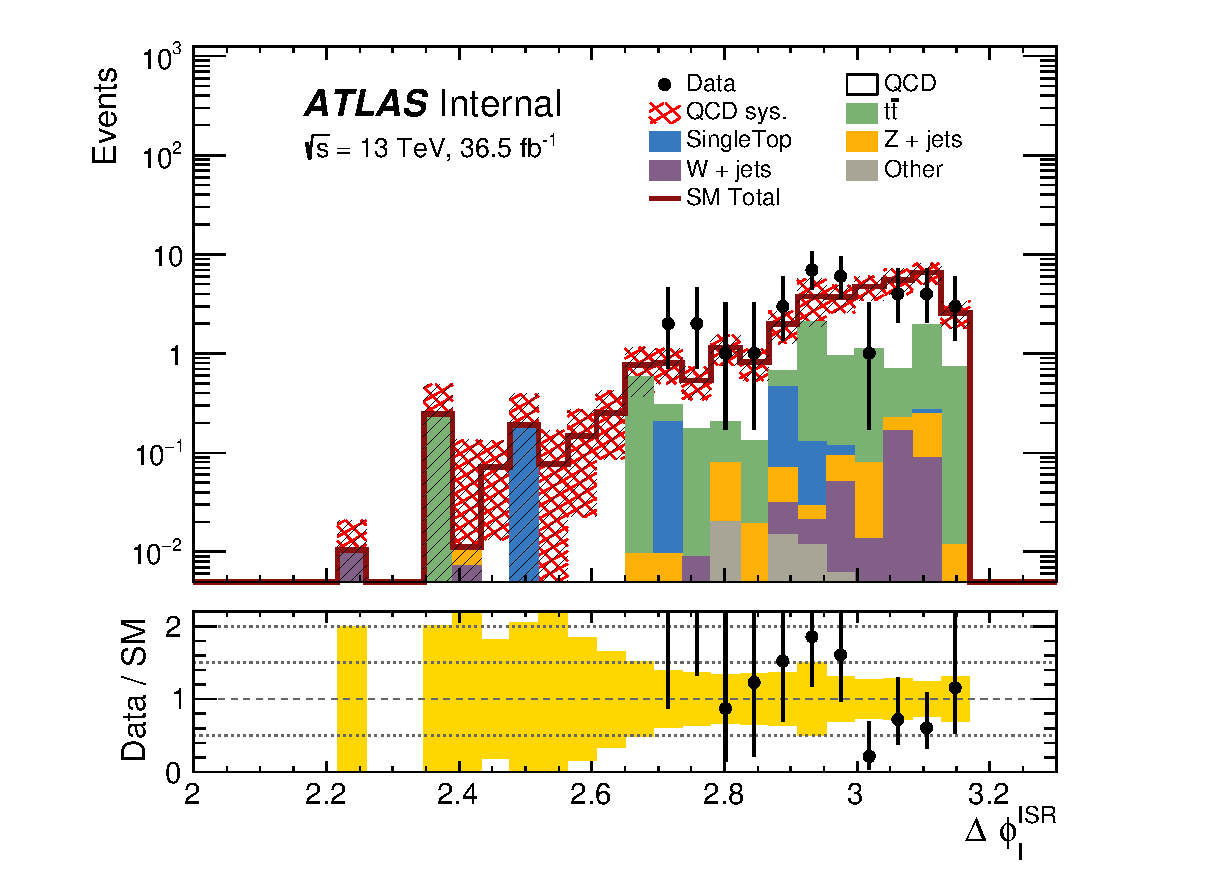
\includegraphics[width=0.48\textwidth]{figures/QCDJetSmearing/CRQC/dphiISRI_36500.eps}
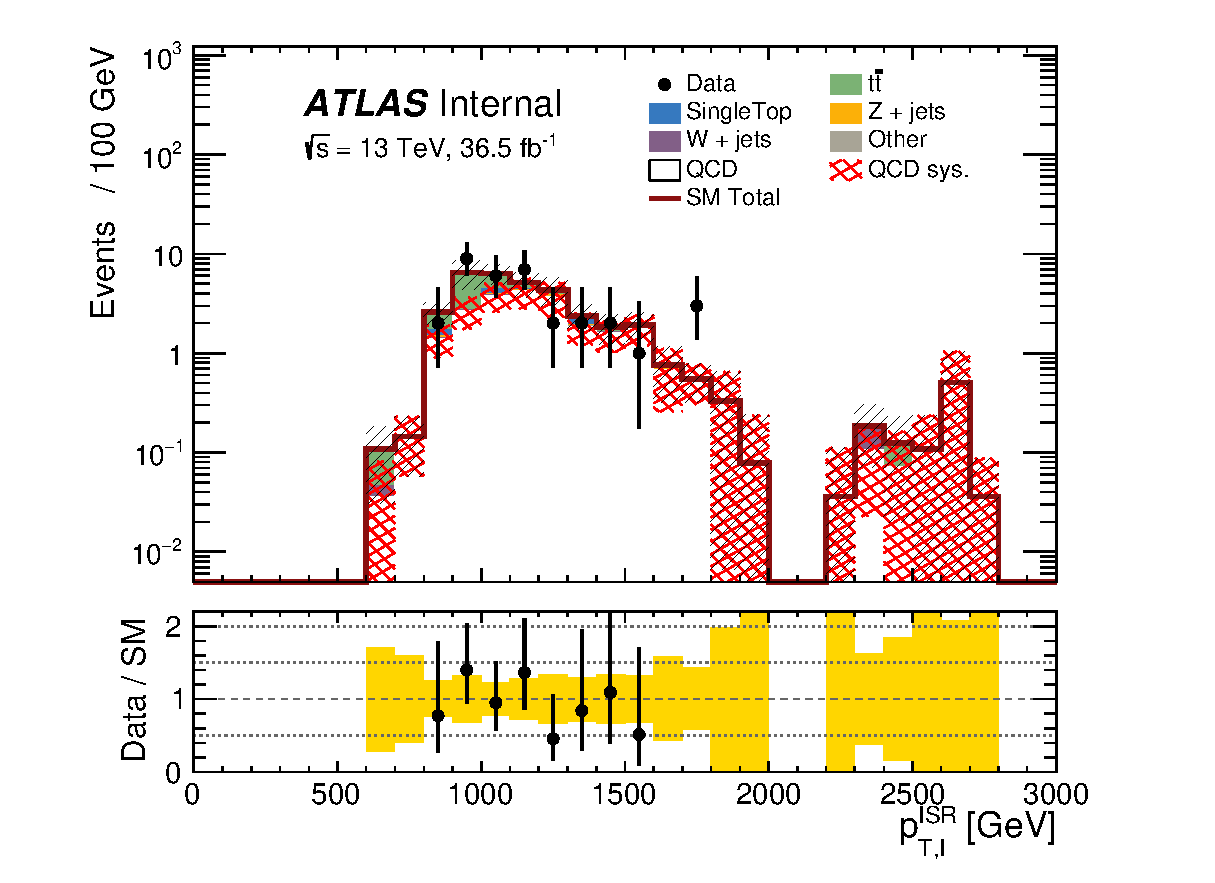
\includegraphics[width=0.48\textwidth]{figures/QCDJetSmearing/CRQC/PTISR_36500}
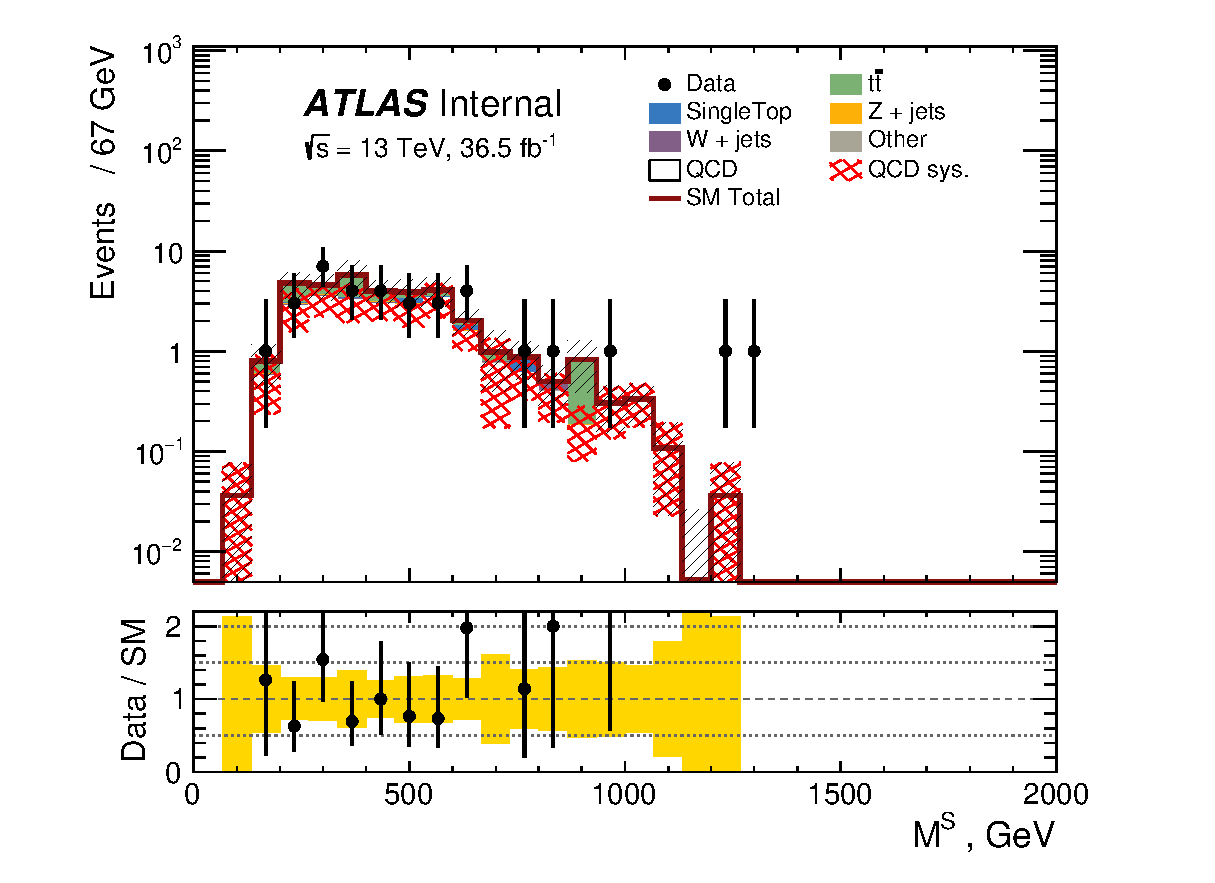
\includegraphics[width=0.48\textwidth]{figures/QCDJetSmearing/CRQC/MV_36500}
\caption{$\PTISR$, $\dphiISRI$ and $\MS$ distributions in the QCD control regions.}
\label{fig:QCD:CR}
\end{center}
\end{figure}

\indent The results of QCD multijet prediction using jet smearing after normalizing to the CR can be checked in the QCD VR defined in table \ref{tab:QCDVR}.   The QCD VR has the exact same kinematic selection as the SR except with a lower $\mindphijettwomet$ between $0.1$ and $0.2$.  $\RISR$ is also required to be below $0.4$ as we don't expect significant QCD contribution at higher $\RISR$.  \\

\begin{table}[htpb]
  \caption{QCD VR definitions, in addition to the 0 lepton preselection in Table~\ref{tab:0Lcommon}. }
   \label{tab:QCDVR}
  \begin{center}
    \def\arraystretch{1.4}%
    \begin{tabular}{c|c} \hline\hline
      {\bf Variable} &  VR  \\ \hline \hline
      \mindphijettwomet  &  [0.1,0.2]           \\  
      \nBJetS & $\ge1$ \\
      \nJetS & $\ge5$  \\
      \pTSBZero & $>40\gev$  \\ 
      \mS & $>300\gev$  \\
      \dPhiISRMET &  $>3.00$  \\ 
      \pTISR & $>400$ GeV \\ 
      \rISR  & $<0.4$ \\
      \pTSFour & $>50$ GeV  \\ \hline
       b-tagged jets & $\ge1$  \\ \hline \hline
    \end{tabular}
  \end{center}
\end{table}%

\indent Data vs QCD pseudo-data prediction for the $\RISR$ and $\dphiISRI$ variables for the QCD VR can be seen in figure \ref{fig:QCD:CR}.  A good agreement is found between data and pseudo-data predictions. \\

\begin{figure}[!htbp]
\begin{center}
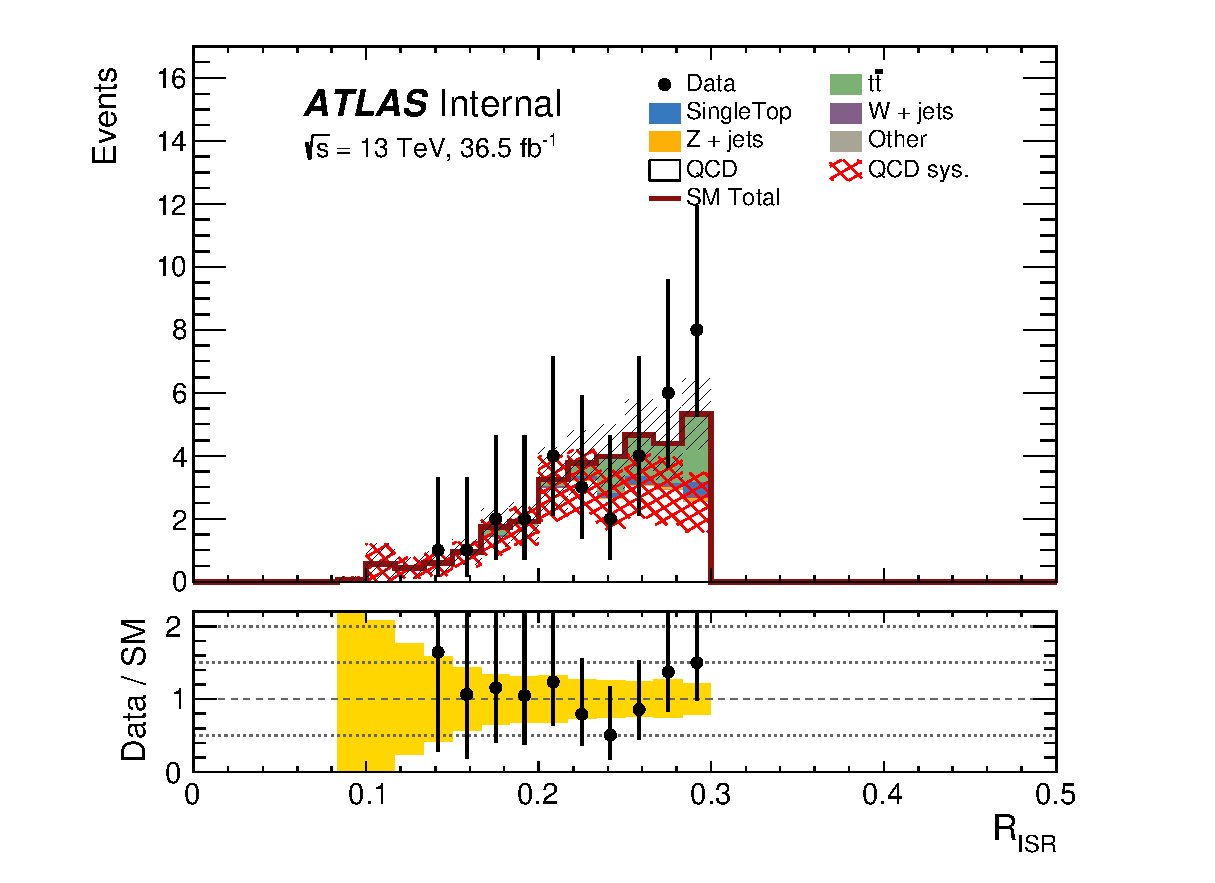
\includegraphics[width=0.48\textwidth]{figures/QCDJetSmearing/VRqC/RISR_36500} 
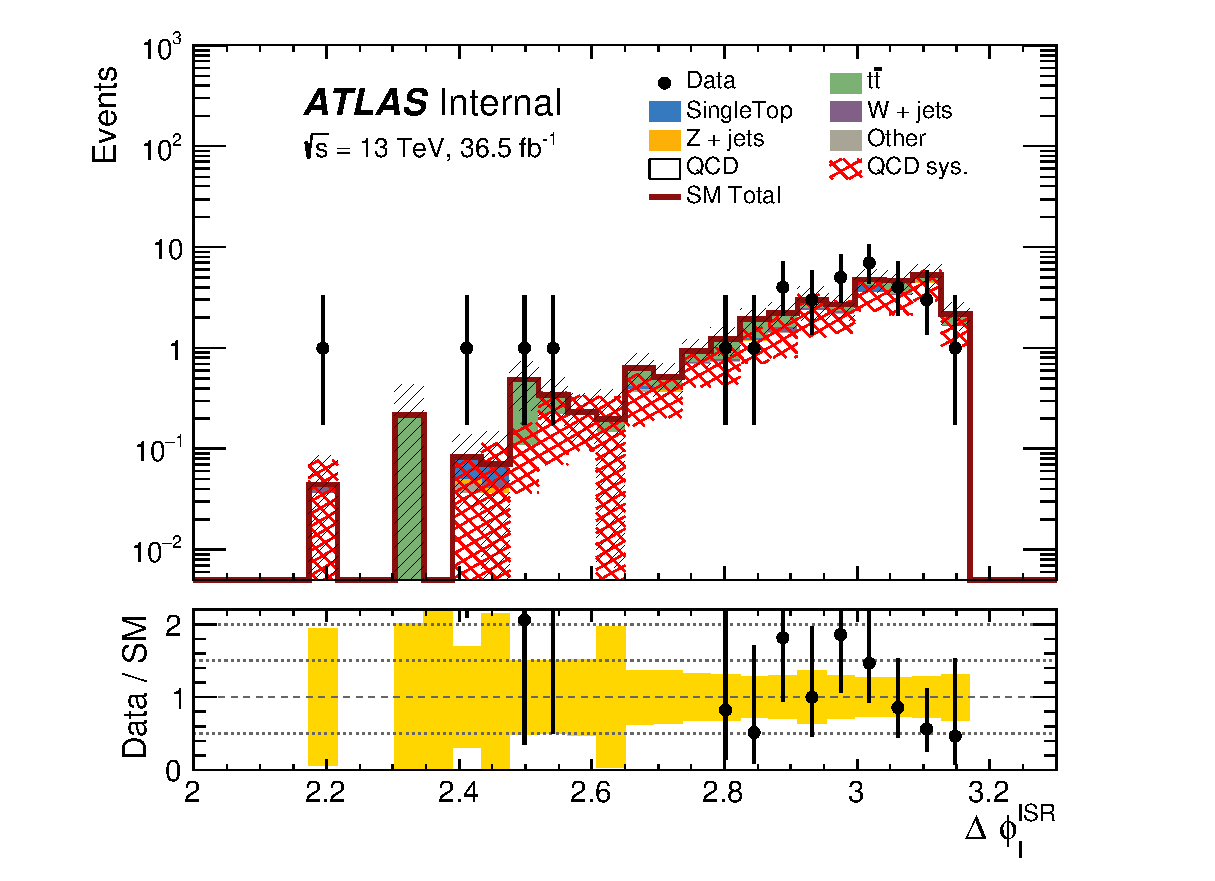
\includegraphics[width=0.48\textwidth]{figures/QCDJetSmearing/VRqC/dphiISRI_36500.eps}
\caption{$\RISR$ and $\dphiISRI$ distributions in the QCD validation regions.}
\label{fig:QCD:VR}
\end{center}
\end{figure}

\subsubsection*{QCD prediction in the Signal Region}

\indent The predicted amount of QCD in the SR is given by the amount of QCD pseudo-data that survive the SR selection after normalization to the QCD CR. The systematic uncertainty on the SR QCD prediction is given by repeating the process with a tighter and looser set of seed event selections.  An upward error correspond to seed events requiring $\met\rm{sig.} < 0.6 + 0.2\cdot n_{\textup{n-bjets}}$ and an lower error corresponds to seed events requiring $\met\rm{sig.} < 0.2 + 0.05\cdot n_{\textup{n-bjets}}$. \\

\indent The expected QCD yield and uncertainty in the SR is given in table \ref{tab:QCD:SRyield}

\begin{table}[!htbp]
  \begin{center}
    \begin{tabular}{c|c|c|c|c|c} \hline\hline
SR $\RISR$ Region       & 0.3-0.4              & 0.4-0.5              & 0.5-0.6              & 0.6-0.7             & 0.7-0.8 \\ \hline
QCD expected yield & $4.56\pm2.38$ & $1.58\pm0.77$ & $0.32\pm0.17$ & $0.04\pm0.02$ & $0.00\pm0.00$ \\ \hline \hline
    \end{tabular}
  \caption{Expected yields of the QCD multijet backgrounds in SR.}
  \label{tab:QCDYields}
  \end{center}
\end{table}%
